%
%	$Id: template.tex,v 2.2 2019/07/26 02:31:32 kato Exp $
%
% KMD Thesis Template
%
% Pick ether \documentclass based on the language you use
% Should work with either pLaTeX or XeLaTeX
%
%\documentclass[12pt,a4j]{jreport}	% Japanese
\documentclass[12pt,a4paper,final]{report}	% English

% Specify your style in comma separated parameters (without space)
%    chicago: use Chicago sytle (otherwise Engineering style)
%    engineering: use Engineering style (default)
%    doctor: use Doctor style (otherwise Master style)
%    proposal: use Proposal style (implies doctor)
%    master: use Master style (default)
%    final: use Final style (otherwise Draft style)
%    draft: use Draft style (automatically becomes final mode
%           in the previous day and the day of submission dues.
%           so don't specify final or draft usually)
%    japanese: use Japanese version (automatically infer from the
%              documentclass style above, and usualy not necessary)
%    english: use English version (automatically infer from the
%             documentclass style above, and usualy not necessary)
%
\usepackage[master,engineering]{kmd-thesis}
\usepackage{pdfpages}
\usepackage{graphicx}
%\usepackage{pdflscape}

%
% If you are going to run LaTeX process in Ovealeaf, you may need to
% upload the files to create a Project. Then, configure the project
% settings by click the gear symble at the top right. In Advanced Build
% Options (left bottom of Project Setting tab), choose ``LaTeX dvipdfmx''
% in LaTeX Engine.
%

%%%%%%%%%% Other tweaks
\makeatletter 
%
% Remove the number from subsection headings
%
%\renewcommand*{\l@subsection}{\@dottedtocline{2}{3.8em}{1.2em}}
%\renewcommand{\thesubsection}{\hskip-1.0em}

% Used to letterspace chapter titles
% adapted from http://stackoverflow.com/a/3951837
%
%\newcommand{\addspaces}[1]{\@tfor\letter:=#1\do{\letter{\,}}}
   
\makeatother

% If you need to use Chinese characters / Korean Characters,
% Uncommend the following 4 lines, and use \Chinese{ } and
% \Korean{ } to represent these characters.
% When you write your thesis in English, such representations
% should be kept in minimum but may be required in Acknowledgement
% and References. Note that you should specify pdfLaTeX as your
% compiler in this case.
%
%
% \usepackage{CJKutf8}
% \usepackage[whole]{bxcjkjatype}
% \newcommand{\Chinese}[1]{{\begin{CJK*}{UTF8}{gbsn}#1\end{CJK*}}}
% \newcommand{\Korean}[1]{{\begin{CJK}{UTF8}{}\CJKfamily{mj}#1\end{CJK}}}
%
% % Examples:
% % \Korean{도쿄}
% % \Chinese{东京}


% Uncomment one of these to change the default Latin font:
%
%\renewcommand*\rmdefault{bch}   % Charter
%\renewcommand*\rmdefault{pnc}   % Century Schoolbook
 
%
% Uncomment to adjust the default line spacing.  The defaults are 1.2.
% Tighter spacing can be used, but this is not really recommended for
% Japanese text.
%
%\renewcommand{\baselinestretch}{1.1}

%%%%%%%%%%%%%% Thesis Parameters - Edit as Appropriate %%%%%%%%%%%%%%

%
% School Year, usually it automatically derived from current date
%
% \syear{2018}

%
% Student Number
%
\studentnumber{82136825}


%
% Thesis Title
%
\title{MotionPerformer: An Ungrounded Haptic Device for Enhancing Self-motion Perception in Virtual Space}

% English subtitle : only when necessary
%
%\subtitle{--- In a Viewpoint of Application Development Platform Environments
%Innovation Generation ---}


%
% Author Name
%    (specify as first name, last name, and capitalize the first letter)
%
\author{Zhou Lu}


%
% Research Advisors
%     First name comes first, and capitalize the top letter.
%     A white space required between first name and last name
%	If the title of your advisor is long, use two lines as following:
%		\addadvisorymember{Project Senior Assistant Professor}{}
%		\addadvisorymember{\ \ \ \ Marcos Sadao Maekawa}{(Sub Research Supervisor)}
\ifDR
   % Ph.D Thesis

\else
   % Master's Thesis
   \addadvisorymember{Professor Kouta Minamizawa}{(Main Research Supervisor)}
   \addadvisorymember{Professor Akira Kato}{(Sub Research Supervisor)}
\fi

%
% Thesis Review Committee
%     First name comes first, and capitalize the top letter.
%     A white space required between first name and last name
%     External Reviewer must be with his/her affiliation
%     When affiliation is too long, use the following format:
%        \addthesismember{Dr. Eiji Kawai}
%            {(Member, National Institute of Information \\
%             && \ \ and Communications Technology)}
%	If the title of your advisor is long, use two lines as following:
%		\addadvisorymember{Project Senior Assistant Professor}{}
%		\addadvisorymember{\ \ \ \ Yun Suen Pai}{(Co-Advisor)}
\ifDR
   \ifPROPOSAL
      % No thesis review committee for Ph.D. Proposal
   \else
   % Ph.D. Thesis
      \addthesismember{Professor Akira Kato}{(Chair)}
      \addthesismember{Professor Keiko Okawa}{(Member)}
      \addthesismember{Senior Assistant Professor Chihiro Sato}{(Member)}
      \addthesismember{Associate Professor Akiko Orita}
                      {(Member, Kanto Gakuin University)}
   \fi
\else
   % Master's Thesis
   \addthesismember{Professor Kouta Minamizawa}{(Chair)}
   \addthesismember{Professor Akira Kato}{(Co-Reviewer)}
    \addthesismember{Professor Matthew Waldman}{(Co-Reviewer)}

\fi


%
% 5 or 6 Keywords
% Each of keywords should be writtn in lowercase letters unless it is
% a proper noun or an abbrevation
%
\keywords{haptic device, self-motion, haptic feedback, sense of agency, automatic system}
%


%
% Choose one submission category from [Design, Science / Engineering,
% Social Science / Humanities, Action Research]
%
\category{Science / Engineering}


%
% Abstract of the thesis
%
\abstract{
The main focus of the thesis is on the development of an ungrounded haptic device called MotionPerformer, which is designed to show the self-motion of a vehicle in virtual space. The device uses a combination of sensors and actuators to provide users with the haptic feeling of motion, which can be used to improve the automation operating system in virtual space. The thesis includes a detailed description of the design and implementation of the MotionPerformer device, as well as an evaluation of its effectiveness in providing the haptic feeling of motion. Overall, the thesis provides valuable insights into the use of haptic devices for self-motion perception in virtual reality, and demonstrates the potential of MotionPerformer for improving the user experience in virtual environments.
}

%
% Acknowledgements in Thesis Language (no \jkmdacknowlegements)
%
\kmdacknowledgements{
Firstly, I would like to extend my sincere appreciation to Professor Kouta MINAMIZAWA, as well as the dedicated team at the Embodied Media Laboratory under his supervision, for their comprehensive support during the course of this research.

I am particularly indebted to Project Assistant Professor Arata HORIE for his expert advice and invaluable guidance in the specialized area of haptics that formed the cornerstone of my research.

Additionally, I am grateful for Project Senior Assistant Professor Yun Suen PAI, whose consistent feedback and insightful direction during the preliminary stages of the design process were instrumental. I also wish to acknowledge the valuable contributions of Project Associate Professor Tatsuya SAITO, who provided crucial support within the context of device application scenarios.

Special mention must be made of Professor Akira KATO for his thoughtful guidance and clarifications, which greatly aided in shaping the overarching direction and methodology of the paper.

Lastly, I am thankful to my peers in the research laboratory, Doctoral Student Ximing Shen, for her instructive input regarding the structuring and data analysis of the manuscript, and Doctoral Student Yulan Ju, whose repeated assistance and contributions to the design process were deeply appreciated.
}

%%%%%%%%%%%%%%%%%%%%%%%%% document starts here %%%%%%%%%%%%%%%%%%%%%%%%%%%%

\begin{document}

\def\chaptermark#1{\markboth{#1}{ }}%
%
% Title Sheet and Abstract
%
\titlepage
\comemberspage
\firstabstract
%
% Table of Contents, List of Figures, List of Tables
%
\toc
\ifPROPOSAL
   % Ph.D. Proposal do not require list of figures, list of tables, and
   % acknowledgements
\else
   \newpage
   \listoffigures
%   \listoftables
   %
   % In English, here comes acknowledgement
   %
   \acknowledgements
   \acknowledgementstext
\fi

\newpage
\pagenumbering{arabic}
\def\chaptermark#1{\markboth{\thechapter.\ #1}{ }}%

%%%%%%%%%%%%%%%%%%%%
% Main Thesis Text %
%%%%%%%%%%%%%%%%%%%%
%
% Here comes main text
%

\chapter{Introduction}
This paper begins by exploring the research background for several key reasons:

Firstly, the focus of this study, Human-Computer Interaction (HCI), is an interdisciplinary domain\cite{paper1}\cite{paper2}\ that necessitates a certain degree of understanding in multiple fields from the reader. By presenting a comprehensive research background, aiming to enhance the reading experience and facilitate a more profound comprehension and reflection on the study's theme.

Secondly, the dissection and exploration of the research theme serve to illustrate the logical progression of this paper more effectively, thereby validating the posed research questions and underscoring the importance of this study.

Lastly, this paper is more than a mere report on the research topic. It encompasses a summary of the extensive efforts undertaken during author's master course. The journey to a clear and definitive research topic included numerous investigations and trials across various fields, an aspect I deem essential to acknowledge and explain within this paper.

\section{Structure}
Chapter 1: Introduction
This chapter primarily provides an introduction to the background knowledge related to the research topic of this study. It encompasses areas such as human-computer interaction, virtual reality and spatial computing, multisensory integration and haptic perception, as well as agency and artificial intelligence.

Chapter 2: Related Works
In this chapter, a comprehensive review of relevant literature on haptic feedback is conducted. The review summarizes previous studies and explores research projects that share conceptual and design similarities with the current research topic.

Chapter 3: Concept Design and Implementation
Chapter 3 presents multiple design iterations leading to the conceptualization and implementation of the MotionPerformer system. The feasibility and potential applications of the system are demonstrated through preliminary experiments.

Chapter 4: Proof of Concept
Two experiments are designed to validate the effectiveness of the MotionPerformer system in terms of force feedback performance and its impact on enhancing agency and user experience.

Chapter 5: Discussion
Chapter 5 analyzes and discusses the research objectives based on the results obtained from the experiments conducted in this study.

Chapter 6: Conclusion
Chapter 6 concludes the research paper and provides a summary of the findings and insights gained throughout the entire master's program.

\section{Human–computer Interaction and Virtual Reality}
\subsection{The Influence of VR Technology on HCI}
Since the concept of Human-Computer Interaction (HCI) was popularized in 1983, HCI researchers have been persistently investigating the proposition of how computers can interact better with humans. From the outset, this theory emphasized that the mode of interaction between computers and humans is different from other tools with limited purposes. Due to its extensive range of applications, the interaction between computers and humans has been analogized to the conversation process between humans.

HCI is defined within the computing community\cite{paper3} as "Human-computer interaction is a discipline concerned with the design, evaluation and implementation of interactive computing systems for human use and with the study of major phenomena surrounding them." Following this definition from the Association for Computing Machinery (ACM), it has been declared that this discipline is also associated with technological developments in computing, human factors disciplines, and even engineering and design methods.

Although the history of HCI's development can be divided in various ways\cite{paper4}, there are a few milestone nodes. In early computer systems, batch processing\cite{paper5e} and Command-Line Interface (CLI) development introduced the concept of early real-time interaction\cite{paper6e}. The advent of Graphical User Interfaces (GUIs), keyboards, mice, and robust underlying infrastructure marked the birth of HCI. The evolution of pervasive computing\cite{paper7} greatly propelled the development of both computers and the concept of HCI.

Nowadays, with the remarkable development of the internet, smartphones, and digital technology, HCI has expanded into areas such as web design and mobile application interaction design. Modern HCI doesn't merely seek usability, it also includes attributes such as user experience\cite{paper8e}, user engagement, and social computing. 

Many papers and articles\cite{paper9} have mentioned that mixed reality technologies represented by VR and AR have once again significantly propelled the advancement of HCI in recent years, especially in the area of user interfaces. For instance, one article\cite{paper10} clearly points out that immersive realities can provide personalized experiences and customized digital content in virtual heritage, which helps to establish contextual relationships between users and cultural backgrounds, and enhances user participation in virtual environments.

Furthermore, related researchers have been discussing how to design and evaluate virtual reality systems based on user needs and experiences, following a human-centered design principle. This continues the development and theoretical support of HCI in virtual reality technology.

\subsection{Spatial Computing of VR}
In the field of computer graphics(CG), we have transcended typical two-dimensional depictions, such as photos or video-quality flat images that can reach resolutions as high as 8K or 12K. While it has not reached the limits of human visual perception, CG industry already possess significant technological capabilities in the image display, which supports the applications of image and video display in our daily lives. In terms of flat image representation or what is viewed through a display screen, our current planar vision is nearly indistinguishable from reality. The counterpart to planar computation is spatial computation, which involves three-dimensional computations and the calculations related to their surrounding environment.

The emergence of the concept of spatial computing is defined in recorded literature as "Human interaction with a machine in which the machine retains and manipulates referents to real objects and spaces."\cite{paper11e} The author emphasizes that objects in spatial computing first need to have value in the real world. Spatial computing relies on objects that already exist in the real world. Unlike in the realms of 3D modeling or digital design, the target objects of spatial computing need real or similar objects as references. In the computational process, not only the position and relationship within the Cartesian three-dimensional coordinate system are considered, but also the representation information of the surrounding environment of the object. Hence, the advancement of spatial computing lies in emphasizing the physicality and spatiality in computation. It no longer treats space as an abstract concept, but as the primary influencing target. This can better combine computers with our reality and has some connections with Digital Twin to some extent.

Thus, as mentioned in the discussions of HCI research professors, mixed reality is just a popular term. The underlying paradigm of mixed reality, spatial computing, is a more valuable concept within the field of HCI. The reason why spatial computing methods represented by VR and AR differ from previous interaction methods, as mentioned in their discussions, is that spatial computing is no longer a two-dimensional representation method.

The relationship between spatial computing and virtual reality technology is complementary. Spatial computing is considered the theoretical starting point of virtual reality technology, while technologies like VR, AR, and MR are considered the current manifestations of the concept of spatial computing in computer science. Users can process and understand information through interaction with the environment, and virtual reality can detect changes in space through various types of sensors and make real-time adjustments, thus providing users with a more intuitive and enriched interactive experience.

\subsection{The Development of VR Technology}
Compared to spatial computing, virtual reality technologies, symbolized by VR, may be more widely known by the general public. In a broad sense, virtual reality encompasses various manifestations, including VR, AR, and MR. All these forms involve interaction methods between real and virtual spaces and utilize spatial computing at their core. As the main topic of this paper is centered around VR, the two related technologies of AR and MR will not be further detailed and discussed here.

Virtual reality technology is the most representative of its kind and the first to have been proven to confer significant benefits to computer development and human societal advancement. There are many definitions of VR. For instance, VR is described as "an interactive and immersive (with the feeling of presence) experience in a simulated (autonomous) world."\cite{paper14} Additionally, similar yet not entirely identical definitions note three features of VR: high immersion, high environmental perception, and high environmental interaction\cite{paper15}. According to these three factors, VR can be classified into three different levels of systems: Desktop VR, Fish Tank VR, and Immersive Systems.

Although the developmental history of virtual reality technology is not explicitly laid out, its milestone developments represent different levels of VR technology. The earliest can be traced back to 1962 when the Sensorama simulator first provided a comprehensive sensory experience that included audio, smell, and touch. In 1968, the Sword of Damocles was regarded as the first VR head-mounted display, followed by commercialized VR devices such as the Dataglove, EyePhone, and Boom in the 1980s. With the advancement and cost reduction of VR technology, modern VR headsets represented by Oculus, HTC VIVE, and PlaystationVR emerged after 2010. To date, as the technology has evolved, the application fields have gradually expanded from gaming and entertainment to education, training, healthcare, socialization, and more. Various innovative technologies related to it, such as eye tracking, gesture recognition, full-body tracking, and even artificial intelligence, are making the VR experience more realistic and immersive.

As pointed out in a report analyzing the popular VR application BeatSaber, user observation and interaction with target objects are gradually shifting from flat screen layouts to surrounding spaces. The article summarizes in a straightforward manner the contributing factors to the sense of reality in virtual technology and the future development direction of virtual technology, which is not confined to a singular visual perspective.

\section{Virtual Reality and Haptic}
\subsection{Multisensory and Synesthesia}

When virtual reality technology was defined, it was emphasized that the sense of immersion in virtual space is influenced not only by visual factors. The definition of spatial computing also underlines that apart from the target object itself, the environment around the target object should also be included in the calculation, including hearing, touch, smell, and so on. A report\cite{paper16} indicates that additional sensory input can enhance the sense of presence in a virtual environment and improve memory of objects within the virtual environment. Adding sensory cues beyond vision may be an effective way to manage the trade-off between the level of detail present in the virtual environment and the frame rate.

The method of providing users with multi-sensory information is referred to in cognitive psychology as Multisensory and Synesthesia. Multisensory and Synesthesia are two similar but not identical concepts. According to relevant neuroscience research\cite{paper17e}, the cooperation or interaction between multiple senses and the fusion of their information content is called multisensory integration, thereby creating a cross-modal stimulus combination. This combination is used to achieve a certain type of response. The latency of this multi-sensory response is significantly shorter than that of any single sensory response. In addition, multi-sensory information sources can enhance or even create a single perceptual experience, similar in effect to synesthesia.

A significant reference\cite{paper18e} in the field of synesthesia interprets synesthesia as a "joined sensation". This specifically manifests when the experience of one sense involuntarily transforms into another sensory experience. For example, in the eyes of people with synesthesia, seeing numbers also assigns colors to these numbers. Tasting and smelling simultaneously enables them to sense additional information such as an object's contour, texture, weight, and temperature. Like multisensory, establishing artificial synesthesia in a virtual reality environment through multimodal methods can significantly enhance immersive VR's performance in system guidance and directing user attention\cite{paper19}.

\subsection{The Necessity of Haptic Technology}
Both spatial computing and multisensory experiences, these leading research trends indicate that in the future development of VR, traditional human-computer interaction that merely uses planar graphic interaction and audio-visual information will not suffice to express the sense of immersion required by virtual reality technology. Several articles\cite{paper20}\cite{paper21} mention that haptic feedback is essential to enhance the immersion and interactivity of VR systems. At present, major commercial VR games or VR videos only provide good visual and haptic feedback, while the perception of haptic information is primarily through vibration.

In addition to enriching perceptual capabilities, another necessity for the development of haptic sensation is its initiative. In other words, haptic sensation should be actively emitted for a certain purpose or behavior. Put differently, haptic information is not only input information received by the user, but also carries input functions different from vision and hearing. The information contained therein varies depending on the user's usage scenarios and intentions. How to analyze integrated information and select the needed haptic information for users\cite{paper22} is one of the main topics in the development of haptics.

Moreover, in classic multimodal structures, haptics serves as a bridge linking various perceptual information. For instance, it conveys the shape, size, roughness, temperature, and so forth of an object to the user through tactile touches and grasps. This interaction process often requires users to actively choose. In general, in a complete multimodal perception structure, multimodal perception needs haptic to provide an information source to enhance the quality and depth of multimodality.

\subsection{Development and Application of Haptic Technology}
Similar to human-computer interaction, the development of haptic technology can also be roughly divided into three stages\cite{paper20} based on the development of personal computer technology:

\begin{enumerate}
    \item \textbf{Desktop Haptics}: Desktop haptics is mainly used in desktop environments, typically provided by a mechanical lever with a certain degree of freedom to provide feedback of some real physical touch sensation, such as the shape or resistance of the target object. The design goal mainly focuses on surgical simulation or mechanical operation training.

    \item \textbf{Surface Haptics}: Surface haptics primarily targets platforms such as smartphones and tablets, dedicating to creating direct contact information between fingers and object surfaces, for instance, fingers can feel the contour and roughness of the object surface. An example of this is the mechanical vibration widely applied on mobile phones today. When pressing a button on the screen, the phone generates corresponding vibration, thereby simulating the interactive behavior between the finger and the real button.

    \item \textbf{Wearable Haptics}: In recent years, with the development of VR technology and the gradual popularization of commercial VR equipment, how to provide force feedback for the entire hand in the VR space, and support more detailed operations like touching, grasping, and manipulation through different gestures under the full freedom of fingers, has become a pressing question. The main research trend at present is haptic gloves. Major technology companies have launched their versions, but the specific features and standard requirements for force feedback gloves have not been clearly defined. In addition to the more idealized haptic glove solutions, there are many haptic schemes that have chosen fingertip feedback devices, handheld feedback devices, and controller-type force feedback devices. However, they all share the same goal: to provide users with gesture interactions in virtual space that are as similar as possible to those in real life.
\end{enumerate}

\section{Haptic and Automation}
\subsection{Telexistence and Artificial Intelligence}
Virtual reality technology not only can be used to create virtual scenes for users, but its high immersion and interactivity can also transmit user scenarios across space. For instance, users can achieve remote work at home using head-mounted displays. The combination of virtual reality technology and robotics can achieve a physical presence. Especially during the COVID-19 outbreak period, which significantly impacted users' activities and contact behaviors, many researchers are committed to combining VR, haptics, and robotics to establish a telesensation control system, also known as remote presence or telexistence. 

Differing from previous remote presentation systems\cite{paper23}, modern remote presence systems actively use multisensory sensors. They not only provide an immersive experience in terms of audio-visual effects but also generate actual physical interactions, such as touching, manipulating, and grasping, amongst other complex movements. The specific forms of manifestation are no longer limited to humanoid robotic devices. There are more flexible forms of existence, such as soft robots, robotic arms, and even wearable types\cite{paper24}.

Additionally, when discussing robot manufacturing, we cannot ignore artificial intelligence, which acts like the brain of a robot. As a core technology with robots, it is not surprisingly being attempted in combination with VR\cite{paper25} or remote presence technology, acting as a control solution when not directly controlled by a user. In the classic artificial intelligence (AI) theory reference\cite{paper26}, AI is defined as "the study of [intelligent] agents that receive precepts from the environment and take action. Each such agent is implemented by a function that maps percepts to actions, and we cover different ways to represent these functions, such as production systems, reactive agents, logical planners, neural networks, and decision-theoretic systems" emphasizing perception and action as two key components. These two components have been repeatedly mentioned in previous descriptions of virtual reality technology and haptic technology. Therefore, when developing remote presence technology, we inevitably need to consider the role that AI plays in remote presence technology and the interaction between users and AI.

\subsection{The Sense of Agency}
With the development of automation and AI, the process of HCI is no longer a single control behavior. The computer will complete the transition from a tool to an intelligent tool. The biggest convenience of technological development is to simplify complex things, such as breaking through the constraints of space and time, making remote things close, and preserving things from a long time ago until now. While simplifying or automating processes improves task efficiency, it also brings many issues, one of which is decision transparency.

Decision transparency refers to the clarity and comprehensibility of the decision-making process. In the context of AI-driven automation industries, it concerns whether the behavior of the current device is determined by AI or by the user. In other words, when users use automated devices, is it the AI system manipulating the entire behavior process, the user themselves, or a joint decision between the user and the AI system? As mentioned in several articles\cite{paper27}, agency is a fundamental and ongoing basis for the interaction between users and the world.

Some studies have already proven that the combination of multisensory elements (e.g., visuomotor and visuotactile) can enhance users' sense of ownership of their virtual bodies in virtual reality\cite{paper28}. However, when users collaborate with AI systems, which also have a strong sense of agency, whether haptics will similarly enhance the connection between users and automated devices, and whether it can enhance the sense of agency, is the main topic of discussion in this paper.

%\subsection{Haptic and AI}

\section{Research Objectives}
\subsection{Research Objectives}
The research in this paper begins with the degree to which users perceive motion in virtual space. After multiple trials and tests, the research target is defined as the moving object in the virtual space, and the perception of motion is precisely targeted to the state of motion of self-moving objects.

We hope that through the mechanical device designed in this research, we can accurately convey to users the mechanical force feedback on the motion state of self-moving objects, including common displacement changes, angle changes and speed changes. This could address the insufficiency of force feedback for the state of moving objects in virtual space. After providing effective mechanical force feedback, we consider whether conveying the motion state of automated devices in an automated operating environment using an AI system can enhance the user experience and sense of agency. The aim is to explore the feasibility of implementing rich haptic technology and whether effective rich haptic technology can enhance the interaction between users and intelligent systems.

\subsection{Iteration of the research objectives}
The goals of this research were not precisely defined in the early stages of the project. With the core ideas and keywords (virtual space, spatial computation, haptic feedback, motion perception) fixed, the research objectives were refined or reinterpreted, including the following phased research objectives or research questions:

\begin{enumerate}
    \item Researching the design of a haptic device for delivering force feedback of the parrying actions to users in virtual space.
    \item Exploring how to simplify haptic devices for conveying physical cues to users and exploring expanded application scenarios.
    \item Researching and analyzing current trends in haptic devices in terms of research and design, and exploring solutions that align with the research objectives.
    \item Researching the design of a haptic device for conveying the motion state of moving objects in virtual space to users and validating its effectiveness.
    \item Investigating whether the use of haptic devices for motion state cues affects the user experience and interaction patterns with automated devices equipped with an AI system.
\end{enumerate}

%\subsection{Theoretical Model}
\chapter{Related Works}

\section{Haptic Survey and PA Model}
In the past literature or survey related to haptics, various kinds of haptic devices and their characteristics are extensively mentioned. However, each classification is different. A detailed report on haptics\cite{ref_S001} pointed out two critical factors for judging and measuring haptic devices: \textbf{Physicality} whether the physicality of the haptic device is consistent with the target object, and \textbf{Actuation} whether the device relies on servo drive to achieve haptic effects. 

\begin{figure}[h]
\centering
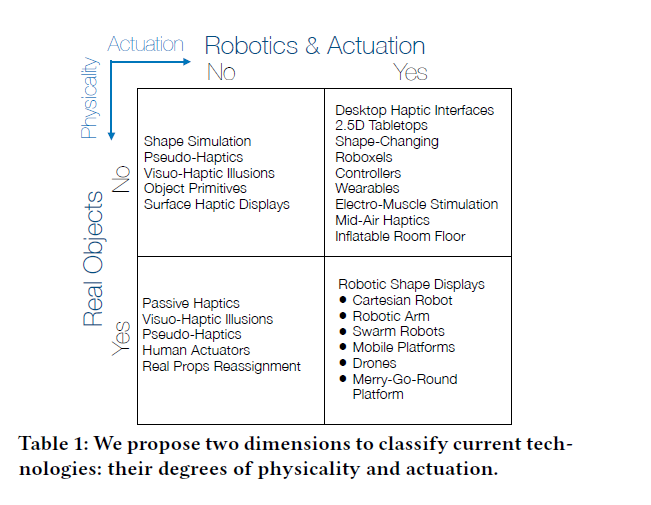
\includegraphics[width=0.8\textwidth]{A_thesis/figures/001.png}
\caption{PA Model}
\end{figure}


Based on these two features, all haptic technologies are divided into four parts. For instance, haptic technologies involving shape simulation firstly do not have devices physically inconsistent with the target object. And since it's based on the theory of force visual simulation, there are no servos or motors used in the entire device, thus falling into the first quadrant (NN). Haptic technology widely used for achieving goals through robotics, such as using a robotic arm to achieve the haptic simulation effect of virtual space objects, is classified in the fourth quadrant (YY) because both physicality and actuation are the same as the target object. As for single-performance focus, for example, in the third quadrant, haptic technology shows the same physical properties as the target object, but does not use driving technology. Techniques such as pseudo-touch and visual-touch technology mostly show different effects based on changing visual parameters (lighting, texture) or tracker display effects (Optitrack, HTC trackers).

\begin{figure}[h]
\centering
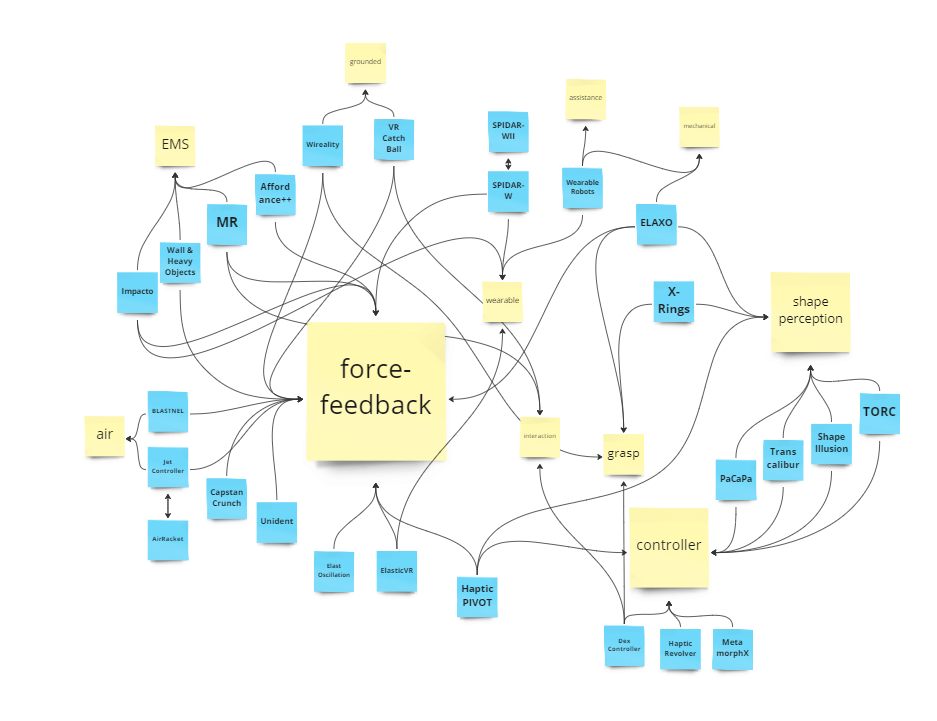
\includegraphics[width=0.8\textwidth]{A_thesis/figures/002.png}
\caption{Rearrangement of multiple references}
\end{figure}


\section{Research Objectives}
Although the PA model theory mentioned above can be used to categorize haptic technology, the initial consideration of this research theme is more inclined to the feasibility of using some robot technology for implementation cost. However, the research purpose will not be the same physical effect as in reality. Therefore, although the PA model has supplemented theoretical knowledge, it does not have a significant effect on its research analysis. After referring to the PA model, according to the research objectives of haptics, the related haptic technologies are divided into the following four areas: object properties reproduction, user Action Assistance, mechanical process performance, and innovative interaction methods. The logic for judgment is as follows:
\begin{enumerate}
    \item Whether there are already existing interaction patterns in reality ?
    \item Whether it is necessary to display haptic effects with multiple different virtual items ?
    \item Whether the user's actions in the usage scenario are dynamic ?
\end{enumerate}

\begin{figure}[h]
\centering
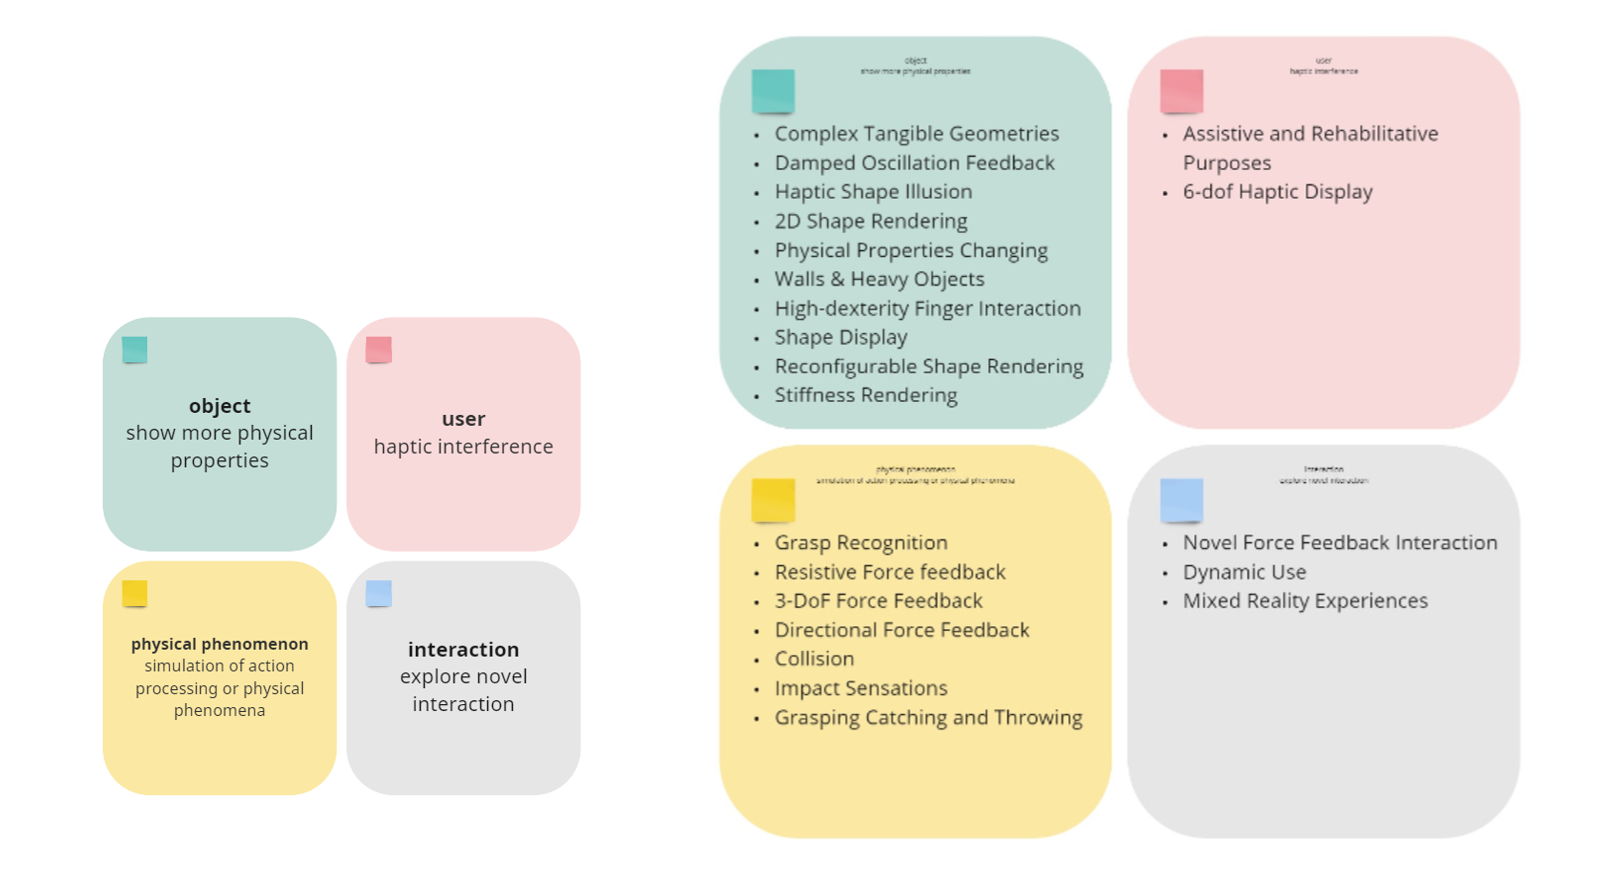
\includegraphics[width=0.8\textwidth]{A_thesis/figures/003.png}
\caption{Classification by research objective}
\end{figure}

\subsection{Object Properties Reproduction}
Haptic devices in this category mainly target virtual objects, aiming to generate or change new object properties. For example, using a cable to fix the user's hand and body to maintain a certain range to make users can feel the outline of complex polygons\cite{ref_003}. By using rubber bands and heavy components to simulate the damped oscillation\cite{ref_006}, it has a noticeable force feedback effect on floating objects and container objects. Using shape illusion to change haptic perception information to simulate virtual objects that do not entirely match the actual shape\cite{ref_012}. Using deformable haptic devices to actually represent handheld items in virtual space\cite{ref_013}. By adjusting the variable torque of CMG devices to show different physical properties such as inertia and viscosity of different objects\cite{ref_017}. By limiting muscles with EMS devices to show heavy objects or walls with large mass\cite{ref_EMS003}. Using the rotation of the wheel to show the texture and roughness on the desktop\cite{ref_MR001}. Miniature devices show the hardness of objects by outputting object resistance\cite{ref_MR004}. By changing the shape of the device to simulate virtual objects of different sizes\cite{ref_MR005}.

\begin{figure}[h]
\centering
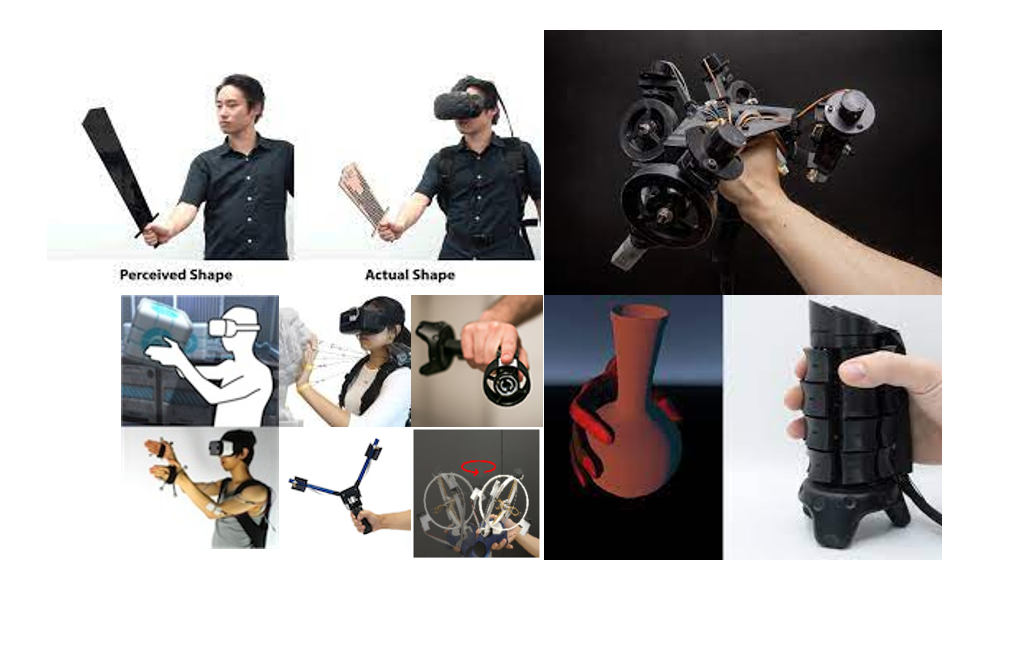
\includegraphics[width=0.8\textwidth]{A_thesis/figures/007.png}
\caption{Research cases of object group}
\end{figure}

\subsection{User Action Assistance}
Corresponding to objects is the impact that mechanical devices have on users themselves. Note that no virtual items are involved in the use and operation of these devices, that is, there are no items as interaction mediums and objects in this type of scenario. These mechanical devices serve not only as action support for users in virtual space but also as auxiliary devices for daily exercise. For example, using hand exoskeletons can enhance user movement in virtual environments and also serve as auxiliary devices for rehabilitation training\cite{ref_002}. Using multiple actuators and fixed devices has achieved the effect of mechanical hints for user positions and movements in virtual space\cite{ref_010}.

\begin{figure}[h]
\centering
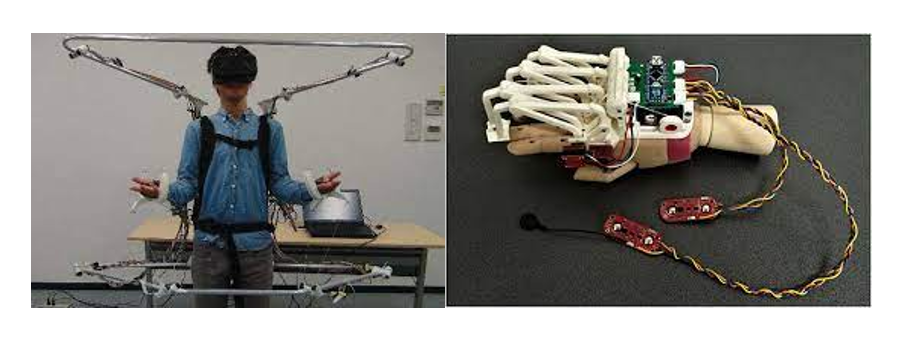
\includegraphics[width=0.75\textwidth]{A_thesis/figures/008.png}
\caption{Research cases of user group}
\end{figure}

\subsection{Mechanical Force Generation}
In addition to focusing on object attributes and user actions, a group of researches pay more attention to the implementation of "force". Force in its basic definition is the result of interactions between two objects. Conceptually representative examples include impact force simulation widely cited using EMS and electromagnets\cite{ref_MR001}. Beyond the usual resistance, by using air propulsion jets to achieve haptic feedback\cite{ref_007}. Also using air propulsion completed directional haptic feedback to enhance the virtual racket sports experiences\cite{ref_008}. As well as compressed air providing full body impact and collision force feedback\cite{ref_015}. Different from contact resistance, continuous resistance has been achieved through rubber\cite{ref_005}. Also, the change of centrifugal force is used to describe the user's grabbing and throwing actions\cite{ref_MR003}. And some of researchers aim to make the resistance as the target, for example, the resistance between two levers is shown through the implementation of two linear motors\cite{ref_014}, simulating the resistance effect similar to scissors\cite{ref_MR002}. Using exoskeleton technology to control and assist palm behavior, describing resistance to achieve actions such as grabbing and twisting\cite{ref_009}.

\begin{figure}[h]
\centering
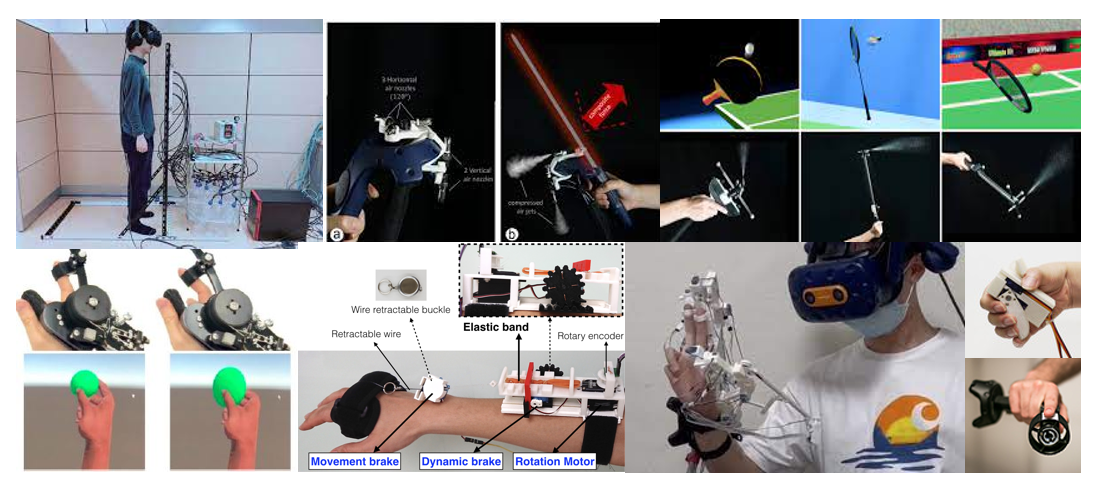
\includegraphics[width=0.75\textwidth]{A_thesis/figures/009.png}
\caption{Research cases of force group}
\end{figure}

\subsection{Innovative Interaction}
There is a category of haptic projects that can be classified according to research goals. Still, because the concepts of these studies are extremely advanced, predictive or creative, some of them cannot be simulated in real life. For example, breakthroughs that give objects interest attributes\cite{ref_EMS002}. And research on the application of haptics in mixed reality\cite{ref_EMS004}. Also the early-stage studies that focused on investigating tactile interaction between users and VR environments significantly contributed to our understanding of haptic perception\cite{ref_001}. All these researches created some more advanced human-computer interaction systems through heuristic haptic technology means. This also inspires us whether we can use new technological means to achieve new haptic experiences we did not have before, and to think about solutions that come with these new experiences.

\begin{figure}[h]
\centering
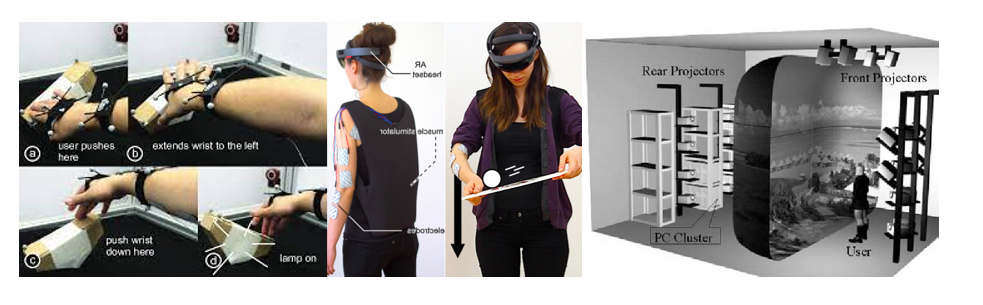
\includegraphics[width=0.75\textwidth]{A_thesis/figures/010.png}
\caption{Research cases of interaction group}
\end{figure}

\newpage

\section{Manifestation Form}
Aside from being classified by research object, device manifestation can also be divided into grounded and ungrounded.

\subsection{Grounded}
Grounded devices are physically connected to external devices or fixed to a static structure, such as the ground or a desk. Usually, grounded devices require large external devices such as air pumps\cite{ref_007}\cite{ref_008}\cite{ref_015}, power supply for driving servos, or base stations required for space trackers\cite{ref_001}. The implementation principles of these devices often involve using robotic arms or similar mechanical structures\cite{ref_010}.

\subsection{Ungrounded}
Conversely, devices that are not connected to external devices are known as ungrounded, and this is the main direction of current research. Compared to grounded devices, ungrounded devices focus more on the manifestation of specific details in virtual space. These devices usually use principles and components such as electronic vibrator\cite{ref_021} or small motors\cite{ref_018}, which require low power inputs, or devices that achieve their purpose through pseudo haptics\cite{ref_S003}. Based on more specific usage, ungrounded devices can be further divided into handheld devices, controller devices, and wearable devices.

Handheld devices refer to those that the user can directly experience with their hand. Handheld devices can be independent devices\cite{paper29}. Some haptic devices are designed to interact with smartphones by attaching to the back of the phone\cite{paper30}.

Controller devices are capable of inputting information while outputting. Common scenarios include adding pneumatic components\cite{ref_007} to existing controls, or embedding sensors in the device itself to provide haptic input such as the degree of grasping force\cite{ref_004}, rather than just joystick or button input.

In addition to these, there are quite a few wearable haptic devices, such as devices that utilize rubber bands on the arm\cite{ref_005} or research that leverages Electrical Muscle Stimulation (EMS) technology\cite{ref_EMS001}\cite{ref_EMS003}. For instance, there are devices\cite{paper31} focused on user wrist movement and force feedback. Such systems can also limit the range of user arm movements while providing haptic feedback.

With the current market development trends, including the heated discussion on the concept of haptic gloves, haptic gloves are also expected to become a new research trend.

\section{Self-motion}
In the mentioned above, we have reviewed many different types of haptic devices. There also have been some studies focused on exploring motion perception. For instance, a fixed mechanical device was used to deliver a force vector to the user's hand and wrist that aligns with the vector direction in virtual space\cite{ref_motion001}. This proved that when force feedback is provided, the user perceives motion information more clearly than when no force feedback is provided. This type of feedback can effectively enhance the user's realistic experience in a virtual environment. However, this project used large grounded haptic devices available on the market. The goal of this research is mainly focused on miniaturization, and on devices that users can use anytime. The study mentioned above demonstrated displacement in a tilt design, which is significantly different from the roller design in this research.

\begin{figure}[h]
\centering
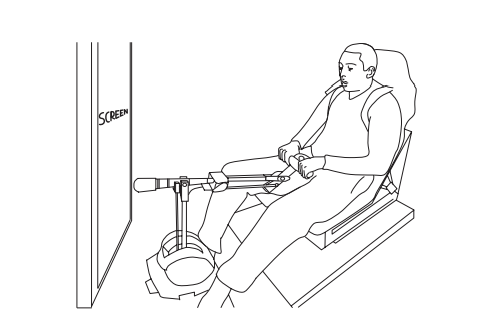
\includegraphics[width=0.6\textwidth]{A_thesis/figures/005.png}
\caption{Experimental apparatus}
\end{figure}


\newpage
Similar research\cite{ref_motion002} has explored whether providing haptic feedback on the rotation vector under passive vision scenarios and only providing visual feedback scenarios would affect the user's judgment of the rotation vector, and whether this impact is positive. In other words, the user's description of the rotation vector under haptic feedback will be more precise than under visual feedback. This is because haptic feedback can help users complete parts of the memory trajectory that did not acquire information. Although the integration of information increases the processing time for users, it enhances accuracy and completeness.

\begin{figure}[h]
\centering
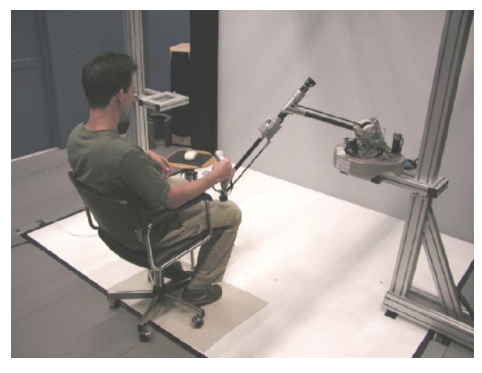
\includegraphics[width=0.5\textwidth]{A_thesis/figures/006.png}
\caption{Experimental apparatus 2}
\end{figure}

\newpage
In addition to the two studies mentioned above, some have designed and produced haptic devices for displaying motion states. For example, one study\cite{ref_motion003} placed a 6dof movable mechanical device at the user's neck and the left and right hands, simulating the user's motion information in a virtual space from the first-person perspective, including linear speed and rotational speed. However, this haptic solution may cause conflict between the vestibular sense information provided by the neck device and the visual information, resulting in simulator sickness. Therefore, another study\cite{ref_motion004} used a rotation vector to express the direction vector of forward or backward, which can effectively reduce simulator sickness.

Some researchers have considered more flexible and multi-purpose design methods. For example, a 6dof freely moving mechanical arm was linked to the manipulated controller\cite{ref_motion005}. Physical pushing and pulling forces such as dragging by the mechanical arm were used to simulate the force situation in the application. This study proved that compared with only using vision, users can more clearly feel their own sense of motion under this method.

\section{AI driving}
Because the application scenario of this research will be designed to simulate the driving environment, after verifying the effectiveness of this design, we will also conduct exploratory experiments and explorations on potential future impacts. This includes whether feeling the vehicle's motion state can enhance the user's sense of connection with the vehicle. For example, in an autonomous driving environment, the transparency of system operation and the responsibility of action consequences may affect the entire autonomous driving interaction system\cite{paper32}, and whether users can trust the autonomous driving system. 

Moreover, with the integration of automated driving systems, how new interaction interfaces and interaction methods develop will greatly influence user trust. For example, the LPD interface\cite{paper33} provided a creative design idea, projecting virtual icons onto the windshield. Another study designed\cite{paper34} a situational awareness system used to detect and adjust the current action mode in real time under autonomous driving environments. Although there is no input/output function for the vehicle's own motion information in the haptic solution, the study\cite{paper35} discussed a haptic design method for adjusting vehicle control in an autonomous driving environment.

\begin{figure}[h]
\centering
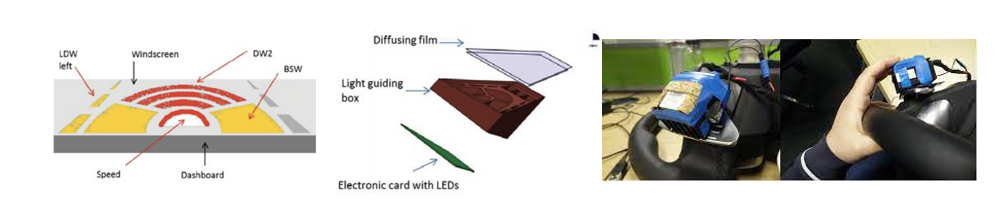
\includegraphics[width=0.8\textwidth]{A_thesis/figures/011.png}
\caption{AI driving related interaction design}
\end{figure}


\section{Summary}
By reviewing the haptics-related papers and articles, we find that most focus on static objects or common mechanical phenomena such as resistance, impact force, collision force, etc. The design preference and implementation methods are mostly ungrounded forms to facilitate user usage, better conform to close the real-world performances, provide more detailed and specific mechanical rendering, and most importantly, allow flexible usage and organic integration with virtual reality technology. For the research topic of this study, although there is no exact solution and topic for displaying the motion state of a self-moving object, many researchers have considered similar topics from different perspectives and aspects.
\chapter{Concept Design and Implementation}
\section{Research Direction}
As mentioned earlier, the scope of the design discussed in this paper has gradually narrowed from a broad scope, but the direction of research and the main key ideas have not changed much, namely how to make users feel their own or the motion trajectory and motion state of the role they manipulate. How can users realize that when they perform a certain action in the virtual space, they are indeed actively doing a certain action spontaneously, rather than just moving their hands or controllers to a specified location according to the guidance of the system. A more abstract explanation is, how can users feel the quality and realism of the action. Can we use some kinematic or haptic devices to convey the action quality of the objects they manipulate in the virtual space to the users, or sufficiently specific action information, to assist users in subjectively or objectively adjusting the amplitude and intensity of their own actions.

Instead of interacting with static objects or those set into motion by external forces, such as a ball being hit, the difference from previous studies is that the target object manipulated by the user in this study has a certain autonomous ability. These are not mere reactive moving state, but self-moving state.

Alternatively referred to as a haptic display device of motion state information for self-moving objects, this technology can be implemented in a wide array of automation systems. These can range from vehicles and drones to robots, or even avatars in virtual environments, thereby opening up extensive applications.

\section{Prototype Version 1 -Katana}
\subsection{Concept Design}
In the initial design attempt, it started with the most common handheld weapon in the virtual environment as a reference and acting object. 

The design goal is to develop a system that can simulate the motion state of the user's handheld object in a virtual environment, such as a weapon. The initial implementation scenario also started with the basic parry action in fencing as the output target. 

This parry mechanism is widely used in action game design, so in the early ideal application scenario, we hope to be able to effectively show high-quality parrying actions of swordsmen through haptic. After the user swings out the controller used as a weapon and successfully parries, the kinematic feedback caused by the recoil force of the parry will be generated so that the user can show the same parrying action interaction as shown in the real swordsman duel.

\begin{figure}[h]
\centering
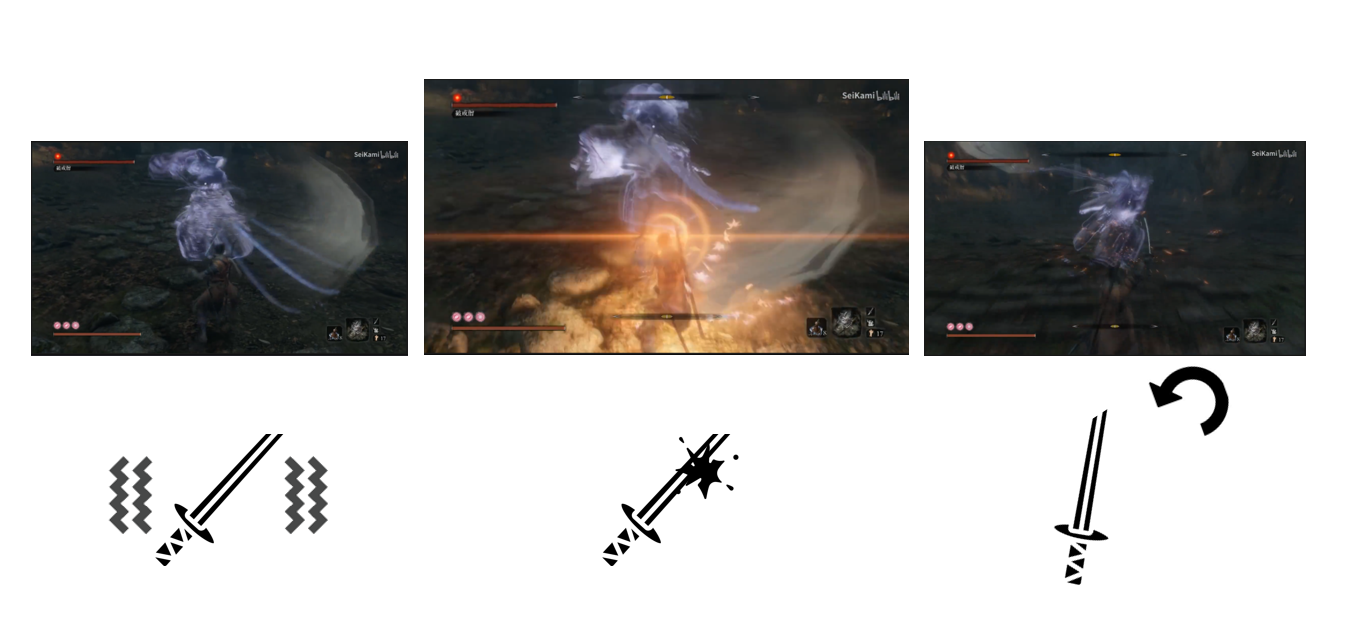
\includegraphics[width=0.6\textwidth]{A_thesis/figures/032.png}
\caption{Ideal scenario}
\end{figure}

In the prototype design, a solenoid is also used as the main source of mechanical output, because the design goal is to simulate the recoil force similar to the impact force. The common driven physical force representation devices in the force output performance can roughly be divided into three types: solenoids, electronic vibrators, and servo motors. The performance characteristics of each type in mechanics are summarized as follows:

Solenoids: Solenoids are electromagnetic devices that generate haptic feedback by generating a magnetic field in a coil by passing current. When current passes through the coil, the magnetic field generates a force acting on the movable chip. Solenoids usually have a larger force output capacity and higher rigidity. Solenoids are frequently used in locking mechanisms including door locking, car parks and access barriers and they are often used in applications that require higher strength and larger displacement ranges, especially as the impact generator.

Vibrators: Electronic vibrators are haptic device that can generate vibrations. It usually consists of a small motor and eccentric mass (such as eccentric rotary mass or eccentric linear mass). When the motor starts, the eccentric mass will cause the device to vibrate, thereby generating haptic feedback. Vibrators usually have smaller force output and lower stiffness, suitable for applications that require rapid haptic stimulation, such as game controllers and haptic notification devices.

Servo Motors: A servo motor is a haptic device that can provide precise force control and position control. It consists of a motor, sensors, and a feedback control system. The servo motor adjusts the output force according to the position information fed back by the sensor to achieve precise force control. Servo motors usually have higher force output and higher control precision, suitable for applications that require precise force control and position feedback, such as surgical simulators and industrial robots.

The prototype design is to set multiple solenoids on one side of the blade of the sword body, use the solenoids to hit the sword body, simulate the impact force generated by the parry in the virtual environment, and force the user to generate a kinematic response.

\begin{figure}[h]
\centering
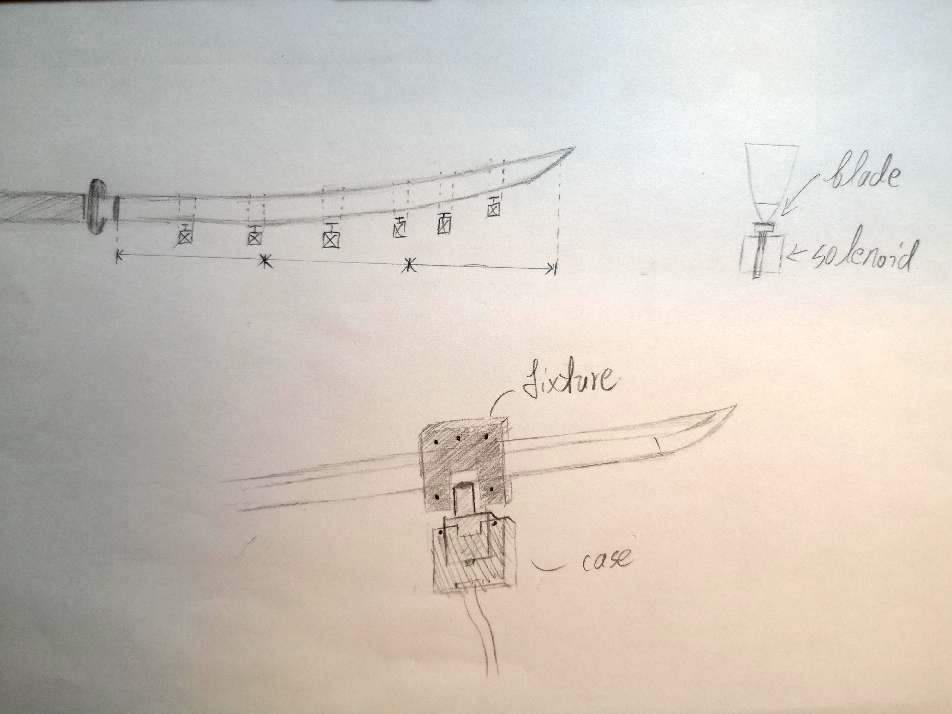
\includegraphics[width=0.6\textwidth]{A_thesis/figures/019.png}
\caption{Early design drafts}
\end{figure}

\subsection{Implement}
\subsubsection{Multi-point Output Control Experimental Circuit}
Considering the principle of voltage shunting, the first attempt is to check whether the 6v circuit on the conventional development board can ensure the output of multiple small 5V solenoids to achieve the purpose of multi-point output.

\begin{figure}[h]
\centering
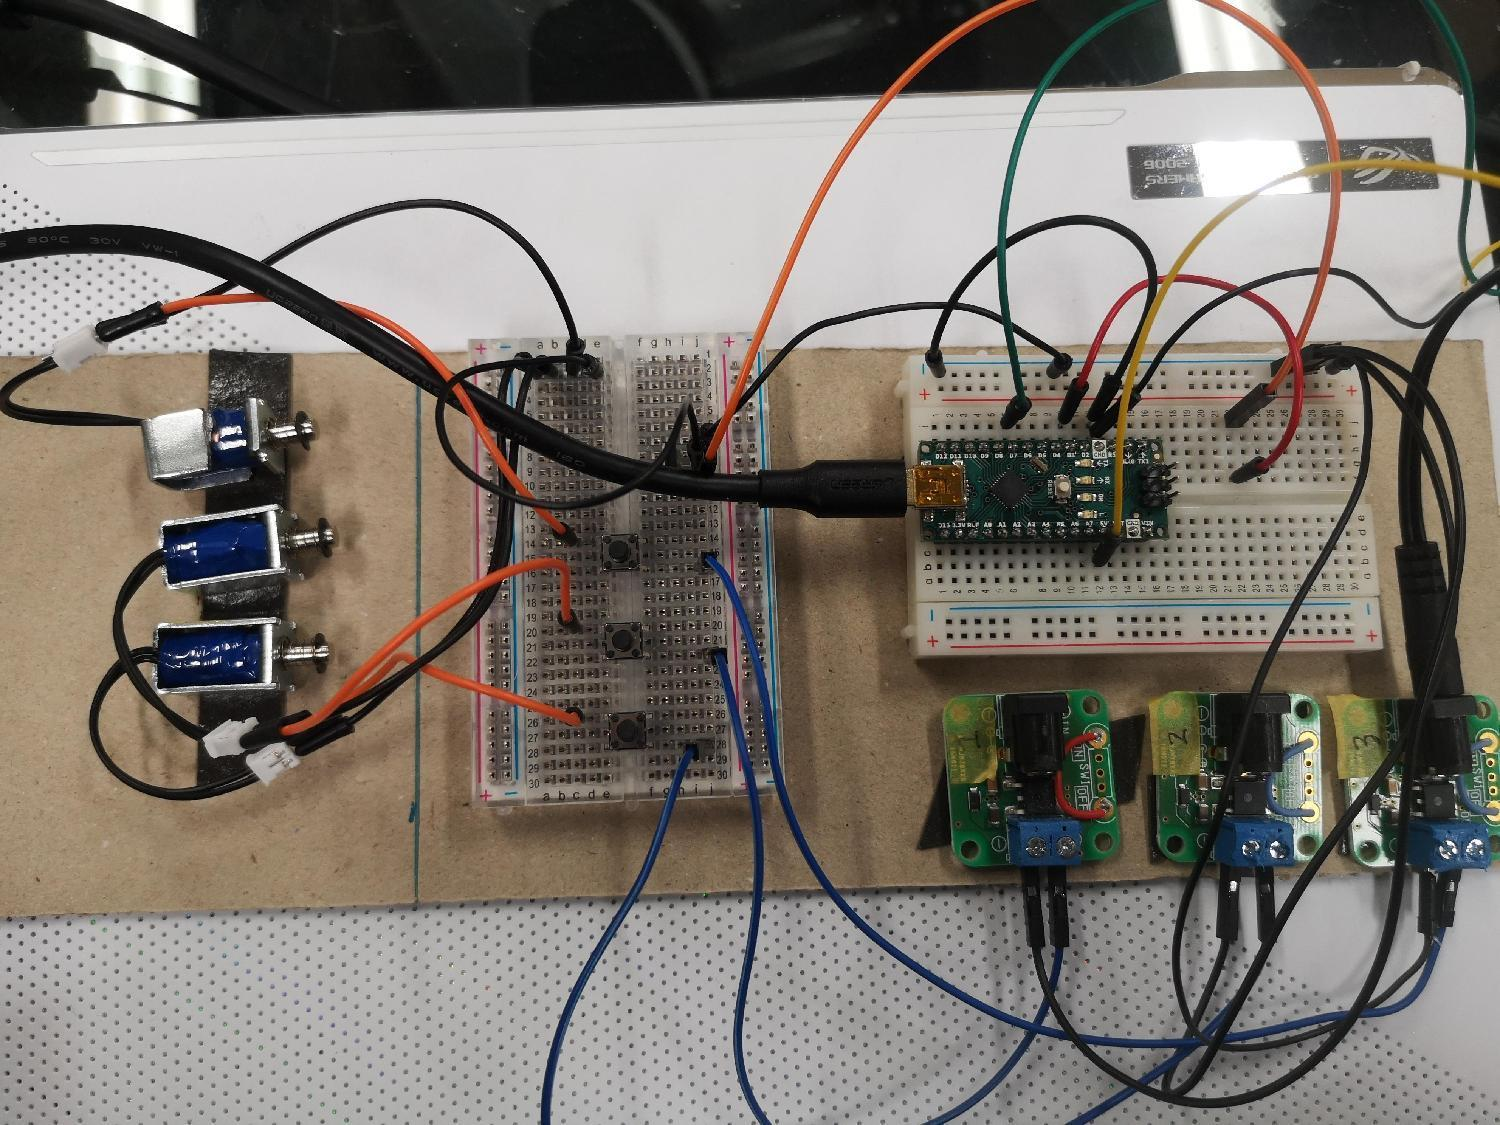
\includegraphics[width=0.6\textwidth]{A_thesis/figures/020.png}
\caption{Experimental Circuit}
\end{figure}

The principle of voltage division, in its practical implementation, has been observed to significantly reduce the standalone power of each component. Therefore, in forthcoming attempts, the primary objective will be the design and implementation of single-point collision detection. This serves as a phased goal, paving the way for further developments.

\subsubsection{Implement Logic Circuit}
The same as the experimental circuit, the initial prototype design also uses the Arduino development board as the main control circuit. At the same time, because we hope that the solenoid device can produce enough kinematic effects, after trying three large-scale, high-output solenoids(12v 1.5A, 24v 0.4A, 24V 1.5A), we chose to use a 24v 1.5A solenoid as the output driver, and used a relay to physically achieve small circuit control of the large circuit, ensuring safety in a high-voltage environment.

\subsubsection{3D Design}
In addition to the core construction, the overall design uses laser printing and 3D printing. To ensure the consistency of the contact points of the solenoids and the blade, laser cutting is used to make the fixtures for the blades.
The solenoids are carried in a 3D printed box under the fixture. At the link point, because no suitable materials were found at the time, only a wooden stick was used as the connector between the two parts.

\begin{figure}[h]
\centering
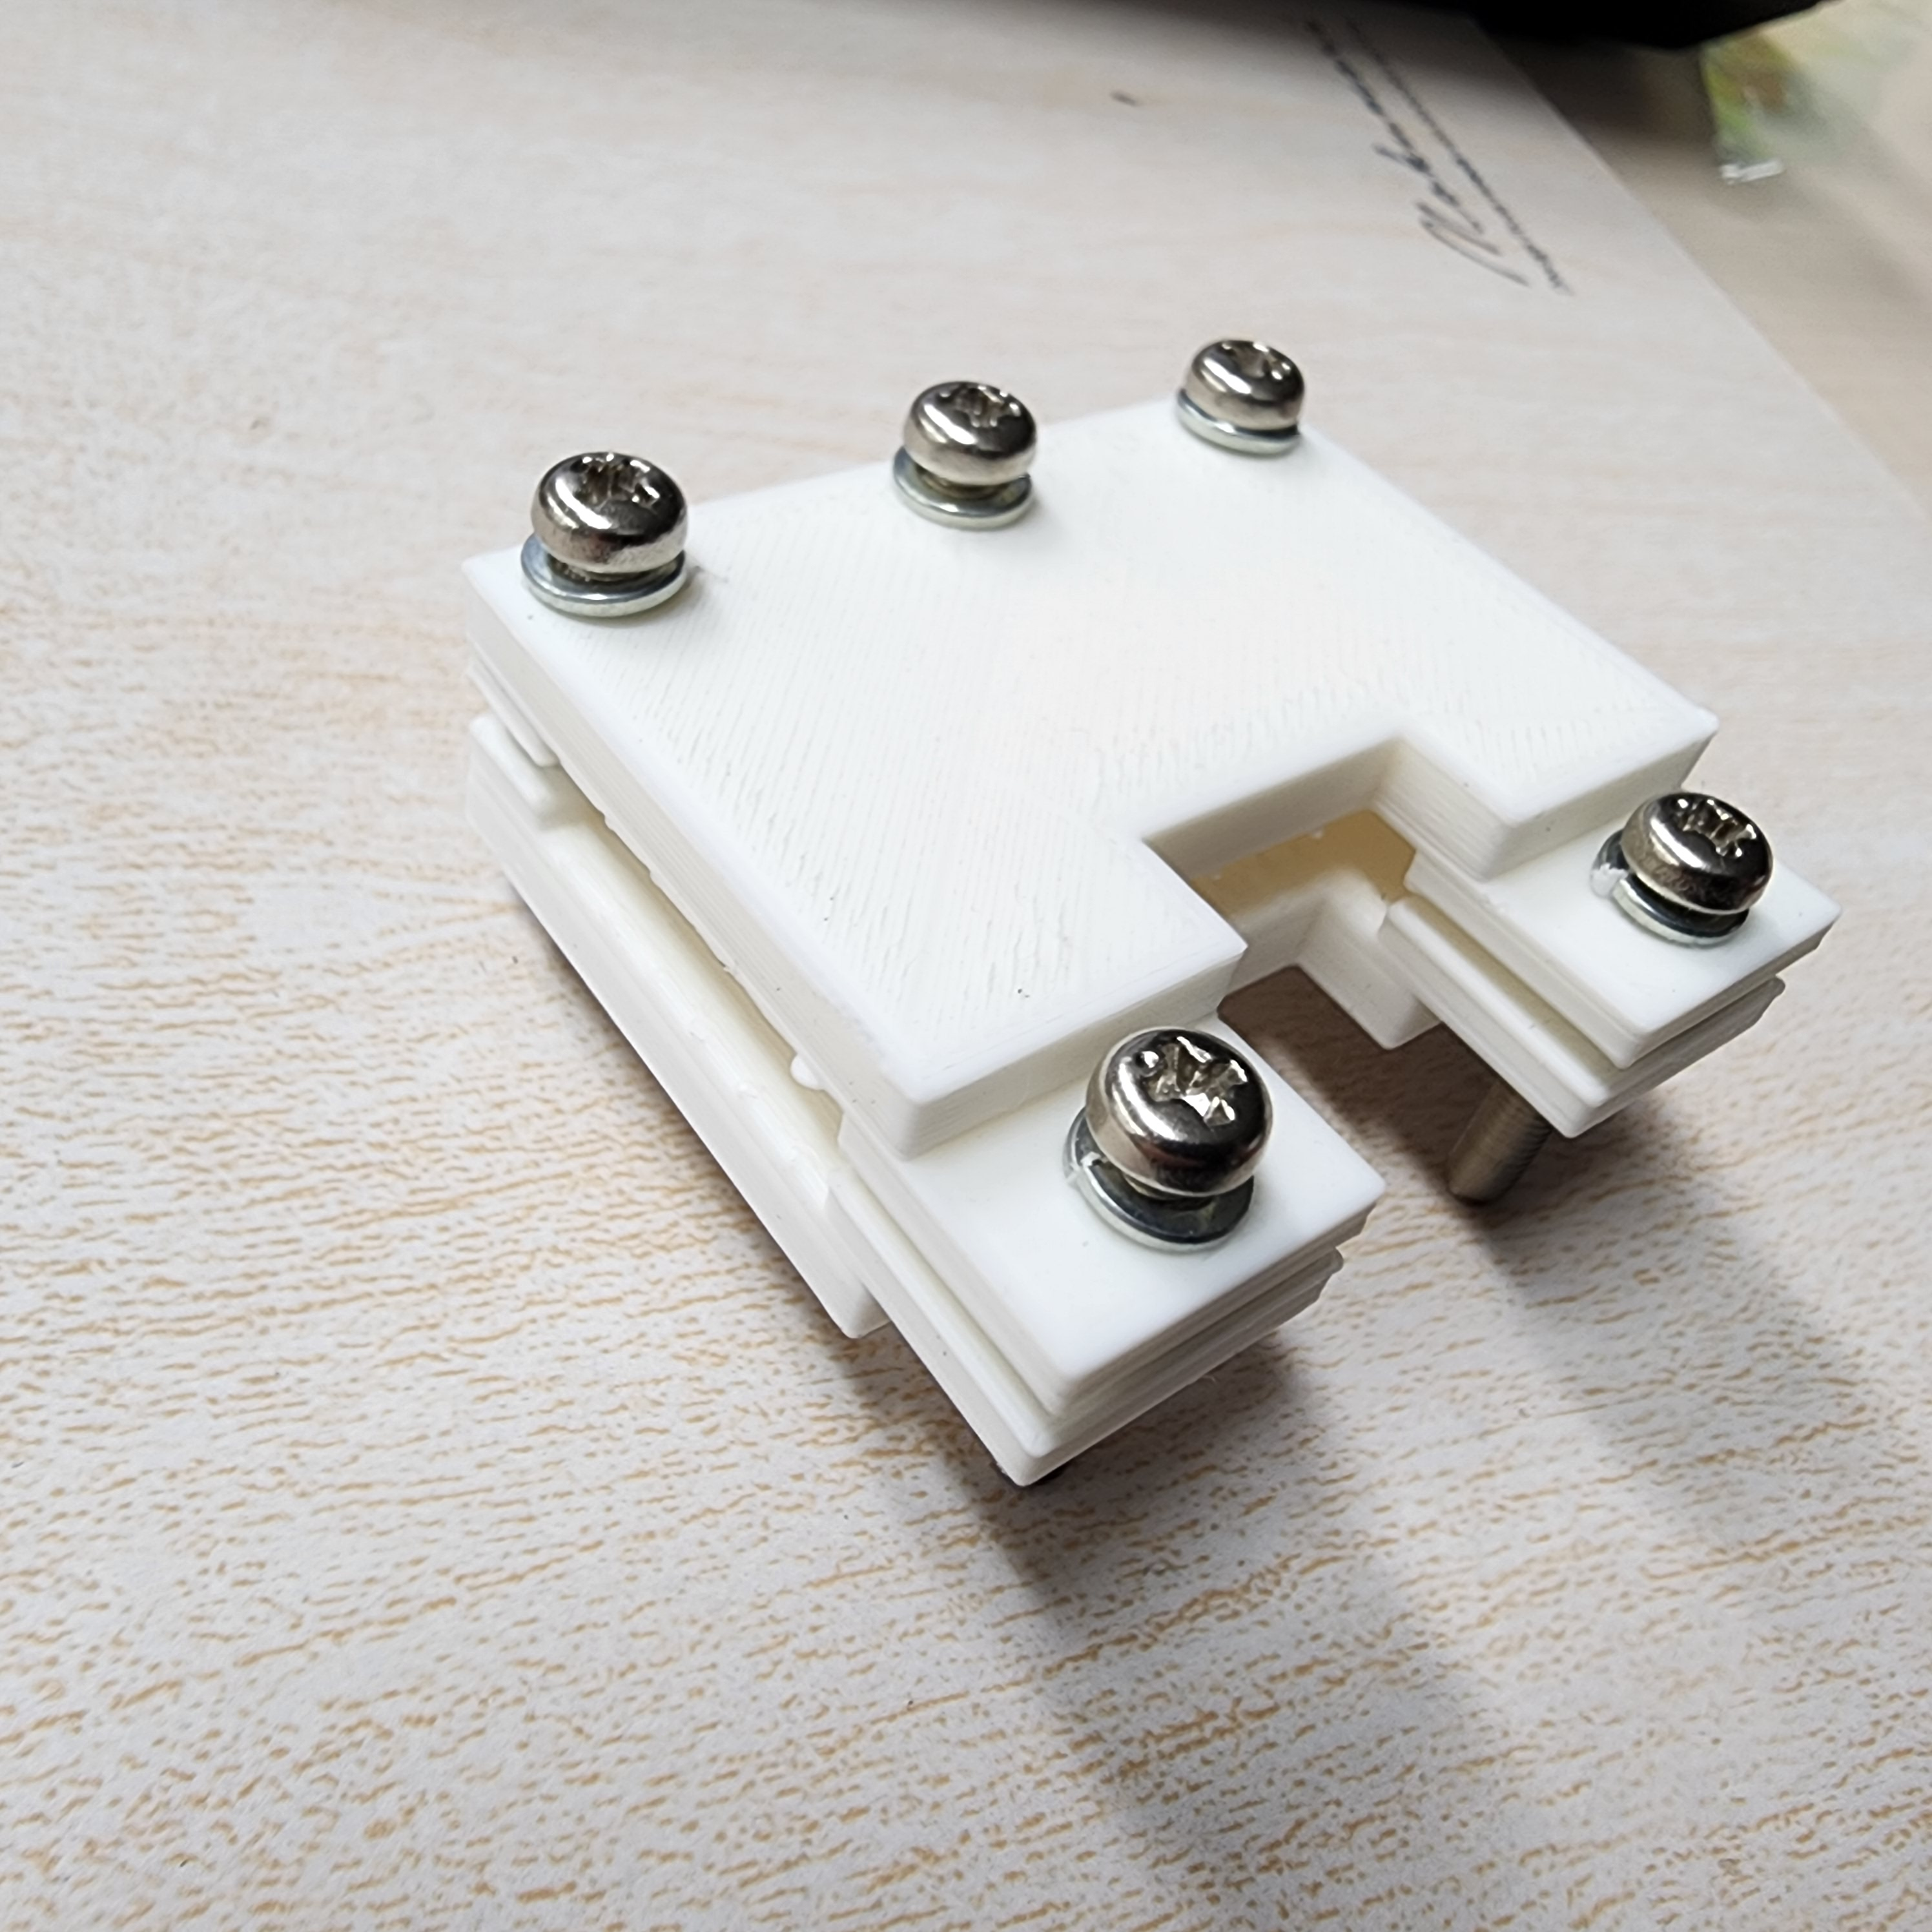
\includegraphics[width=0.6\textwidth]{A_thesis/figures/021.jpg}
\caption{3d design - fixture}
\end{figure}


After production, the device can achieve the most basic blade impact function. In simple terms, the relay is controlled to open and close through the development board, which can control the circuit where the solenoid is located. When the circuit is connected, the central part of the solenoid is pushed back under the action of electromagnetic force, and when the circuit is disconnected, the electromagnetic force returns to the default state, and the central part pushes forward to generate an impact force. The control logic inside the development board is to uniformly control the presence or absence of a digital signal, so that the user can feel a recoil force similar to the collision of swords in the virtual space.

\begin{figure}[h]
\centering
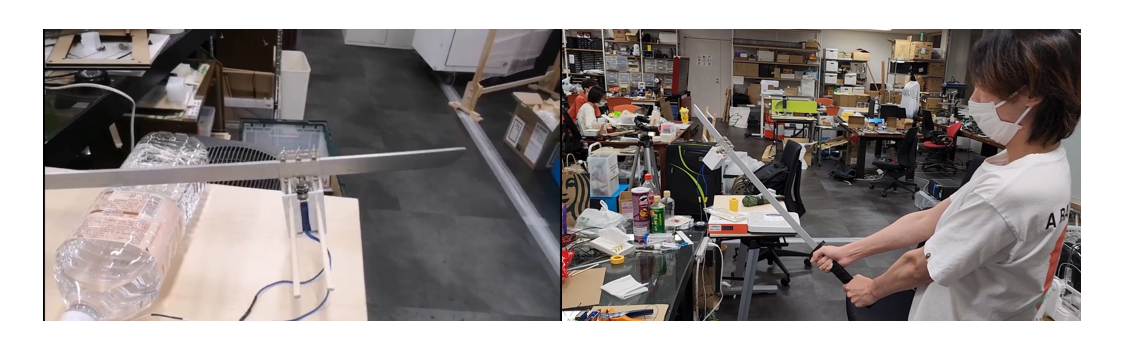
\includegraphics[width=0.95\textwidth]{A_thesis/figures/022.png}
\caption{Prototype and usage example}
\end{figure}


\subsection{Pilot Test 1}
After preliminary testing (n=5), the user's overall feedback was lower than expected.
There are several problems summarized as follows:
The overall weight is large, and the weight distribution is unreasonable. Firstly, the solenoid has a large self-weight. In addition, the hanging area is far from the user's hand grip area. The force arm is too long, leading to a higher design weight, and the weight cannot support the user to use the device freely. 
In addition to not achieving the expected effect in terms of kinematic haptic effects, users strongly suggest that visual information should be used to supplement the deficiencies. In other words, if only using this kinematic device, users are still confused about the application scenario of this device and the specific content of the information conveyed, and need visual guidance.

\section{Prototype Version 2 -zShape}
\subsection{Concept Design}
After the first round of production and testing, the second version of the prototype was modified based on the feedback received. The objective of the device remains consistent with the previous goal, aiming to develop a set that can simulate the user's handheld object movement status in a virtual environment, such as a weapon. The main modifications are as follows:

The device itself does not need to be consistent with reality in terms of length, for example, in the simulation of a samurai sword, the haptic device itself does not need to maintain the same length as the samurai sword. Therefore, the device will not use model knives as the main carrier, but will only use 3D printing to print the device body. The design should consider the user's grip method and pay attention to the tilt angle.
Considering the weight balance, not only the front end of the blade in the design needs a force generator, but also the back end of the device needs a force generator during the recoil process to ensure a certain degree of balance. It won't be too heavy on the front end of the device, making the user unable to control their behavior during use. For the selection of heavy objects, we chose the same solenoid as the front end for adjustment.
Since the existence of the blade is cancelled in the design, it is necessary to consider whether the inertia produced by the solenoid itself hitting the air can produce enough kinematic effects on the user, or use other objects to replace the blade as the impact point of the solenoid.

\begin{figure}[h]
\centering
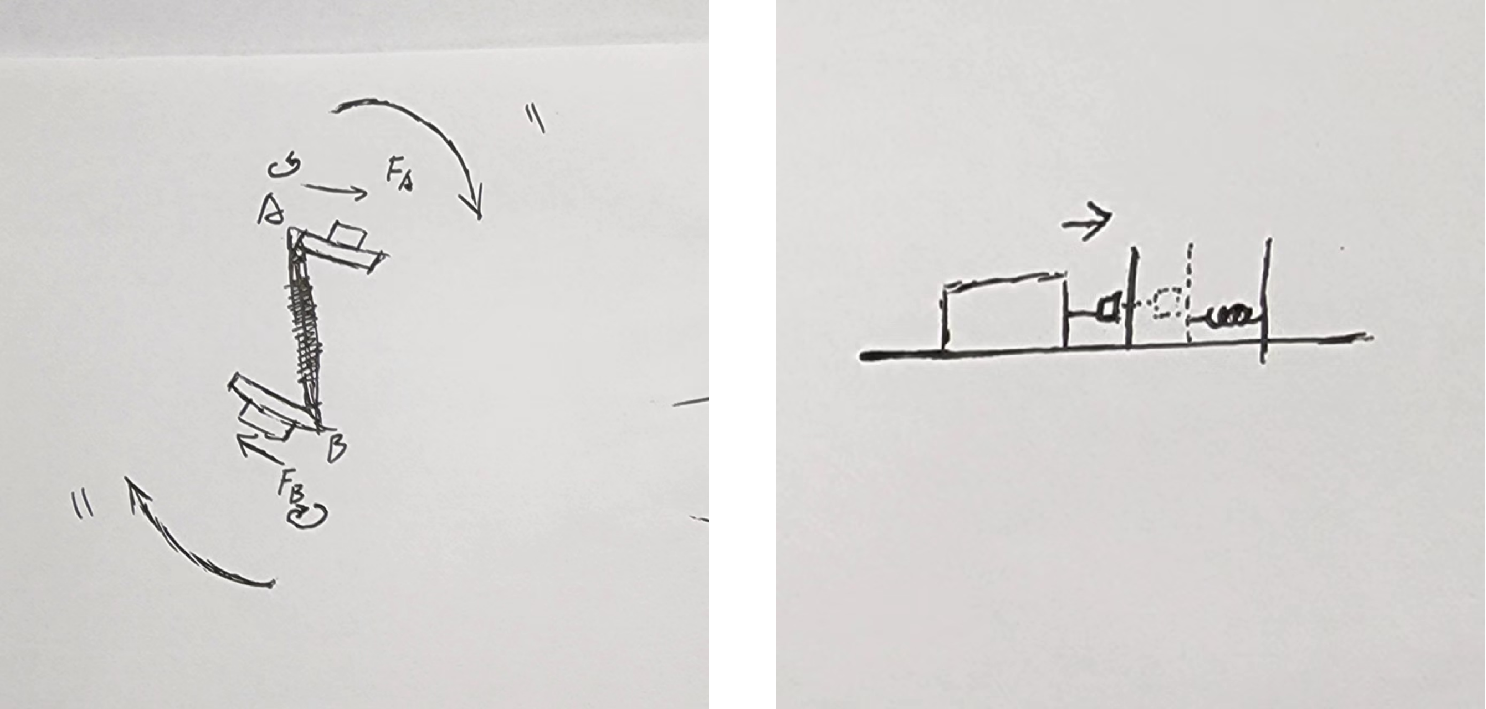
\includegraphics[width=0.6\textwidth]{A_thesis/figures/023.png}
\caption{Early design drafts 2}
\end{figure}

\subsection{Implement}
\subsubsection{Haptic Design}
In terms of heavy object configuration, we chose the same force generator as the previous prototype design, the solenoid, and used the same output model to ensure that the user has the same front and rear weight perception when using it. Also, according to the function design, the solenoid generates output in two opposite directions to simulate the impact force received and the recoil force after receiving the impact force.

\begin{figure}[h]
\centering
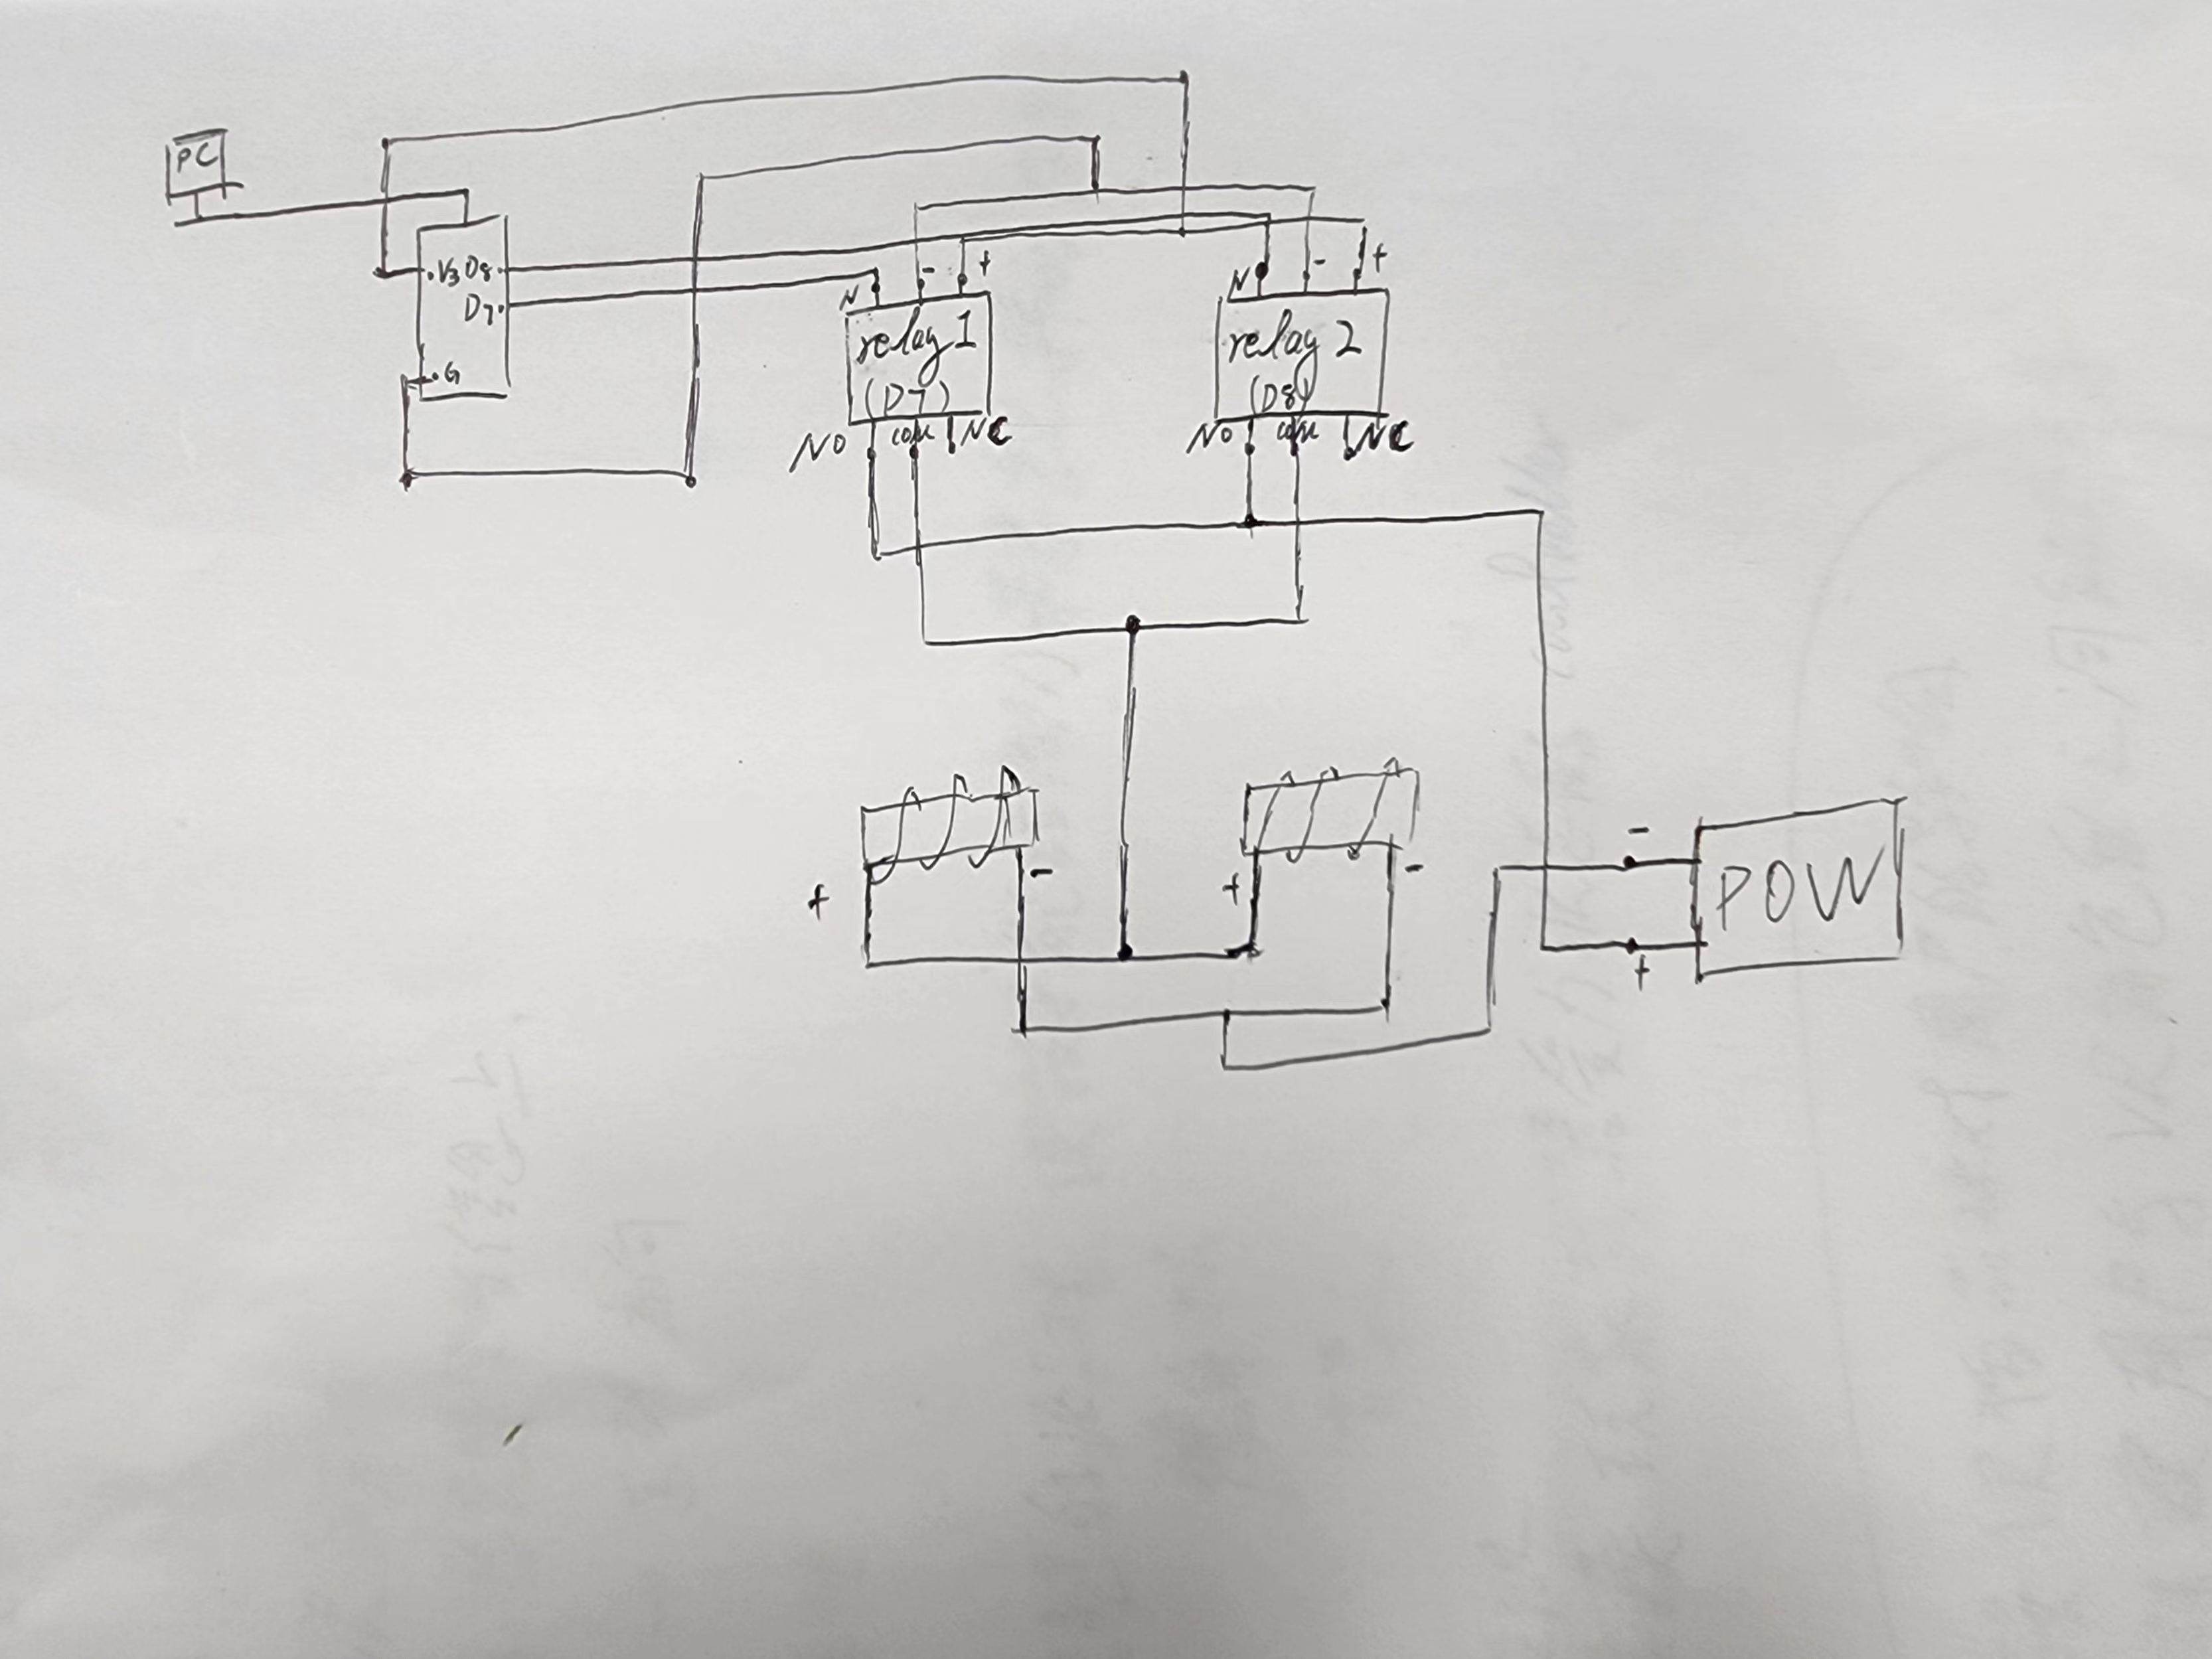
\includegraphics[width=0.6\textwidth]{A_thesis/figures/024.jpg}
\caption{Circuit diagram}
\end{figure}

\subsubsection{3D Design}
For the main body part, we chose a Z-shaped design. The inclined part in the middle is convenient for users to grip and has a certain angle to help the  device better adjust the output. The horizontal structure at the top and bottom is used to provide support for the solenoid base.
In the design of the impact part of the solenoid, a baffle is designed to accept the impact force generated by the solenoid. About the connection method between the baffle and the main body, two schemes have been tried, one is directly fixed to the bottom, and the other is to use rails and springs to make the baffle retractable. Specifically, the rail is dug out inside the base to ensure the movement path of the baffle, and a spring is added inside the rail to restore the baffle to its original position after being hit. However, after testing the actual effect, the kinematic effect of the rail plus the baffle is not as good as the effect of the baffle directly, so the baffle is still fixed on the base.

\begin{figure}[h]
\centering
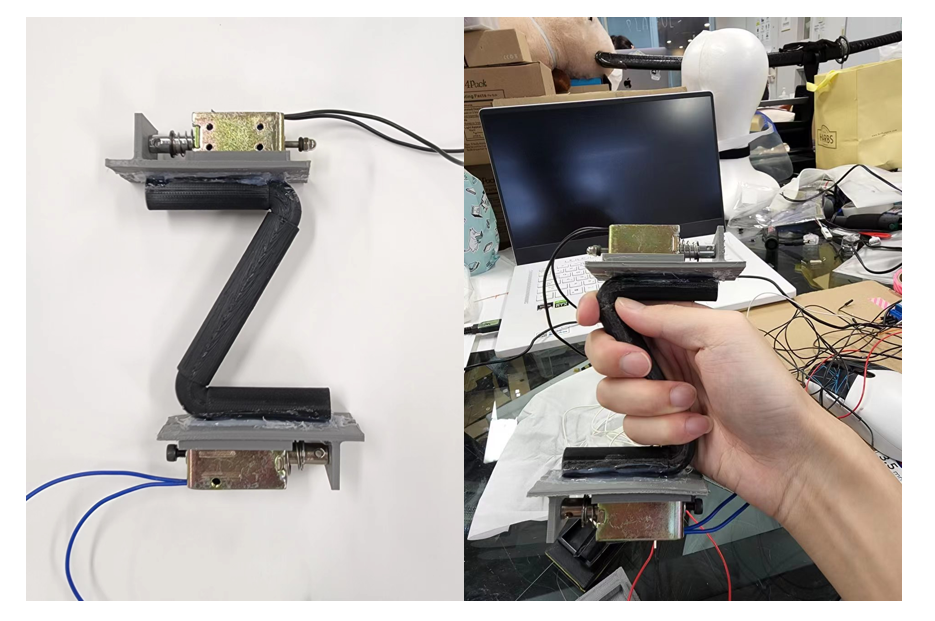
\includegraphics[width=0.6\textwidth]{A_thesis/figures/025.png}
\caption{Prototype display}
\end{figure}

\subsection{Pilot Test 2}
After production, a simple test (n=5) was also carried out. Compared with the previous time, the overall performance has significantly improved compared with the previous prototype, specifically in terms of smaller volume, lighter weight, and better balance. Because the shape is no longer a long strip type, so in the actual application process, the use method and simulation object are no longer limited to long sword-type weapons.
After the two-direction haptic output, the overall movement performance of the device has significantly improved, and people can feel the kinematic effects of advancing and retreating. At the same time, the output in the two directions has a larger adjustment space compared with the single output last time. That is to say, the solenoid can make fine adjustments in its own output mode, such as the solenoid at the rear end fires slightly later than the front end. It may will make the user feel the impact first, then feel the recoil, such a complete kinematic process of receiving force blocking.
However, in the testing process of this prototype, users still cannot understand the purpose of the device without the aid of visual information, and mentioned in the test that "The occurrence of action kinematic effects is very obvious. I know that a certain action has occurred when using the device, but I am still puzzled about what kind of action it is."

\subsection{Conclusion}
In addition to the problems of the device and system itself, there are still three core issues that have not been clearly answered in the entire design process. First, what kind of physical force is this haptic device focused on reproducing? Although the design goal is to hope that users can clearly feel their own action trajectory and direction when using this device, but in the application scenario of weapon swinging, which force is specifically reflected has not been clearly stated. 
Second, the limited application scenario, apart from the user's weapon fighting scene, are there any other potential application scenarios for this system? 
Third, in the design process, it is still a reproduction of the kinematic phenomena that exist in reality, rather than innovative interaction methods on how specific users interact with future technological content. It is necessary to consider some new interaction methods that do not currently exist or may appear in the future.

\section{Drone Research Project}
In addition to the exploration of haptic technology for motion, other research projects have been conducted. While their methods and contents are not the same as the main research topic of this project, they serve as an important reference for the development of future research.
The additional research content here is about using drones as the source of haptic output. Initially, the design was meant to use the 3DOF kinematic output of drones to produce effects on the human body, but it proved challenging to maintain a fixed distance between the drone and the user in the actual algorithm implementation. Ultimately, the drone was fixed on the user's head, and vestibular effects were used to create kinematic effects in multiple directions on the user's head to guide the user to navigate effectively.
In design, we connected the bottom of the open-source drone to a helmet, and the user wore the helmet to feel the physical cues provided by the drone to identify the direction of guidance. To disperse the weight of the drone, a wooden and cross structure was attached to the bottom of the drone and secured to the user's chest.
In the actual experiment (n=5), it was found that the method of guiding the user's direction through the drone could indeed guide the user to distinguish direction. In the second experiment, it was also found that the system could guide the user to the designated location without visual cues and relying solely on touch.

\begin{figure}[h]
\centering
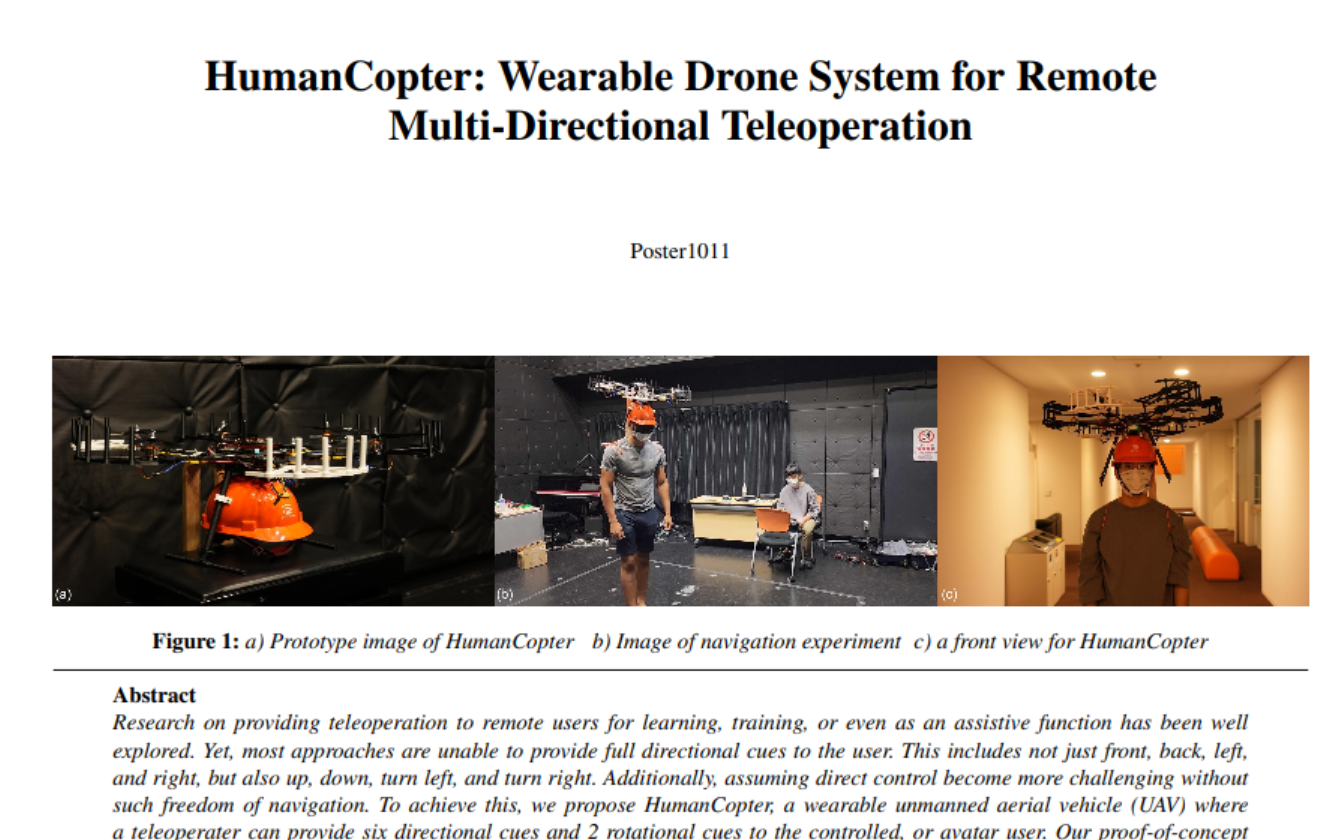
\includegraphics[width=0.75\textwidth]{A_thesis/figures/026.png}
\caption{Publication on drone research project}
\end{figure}


\section{Prototype Version 3 -1dof}
\subsection{Concept Design}
After the previous two attempts, the decision was made to tackle the core problem, i.e., to clarify the research direction. For clarity in the movement trajectory, it might be easier to start with smaller objects with a fixed movement path, such as a train or car that can only move forwards and backwards. Compared to the free actions of users, the human joints have a too high degree of freedom, making it hard to find the basic implementation targets and measurement methods. Therefore, the prototype design of this time started from the most basic movement action to reconsider and design the prototype.
Considering the changes in motion in multiple dimensions, after using the guide rail and tilt designs in previous research, it was found that the tilt design could not effectively represent the accurate distance and feeling of movement in long-term movement. Hence, in the early design of this time, two design schemes were attempted:

Design 1:
Installing three wheels on a handle-like component, each wheel representing movement in one dimension of XYZ, hoping that such a setting could convey the motion information in XYZ dimensions to the user.
\begin{figure}[h]
\centering
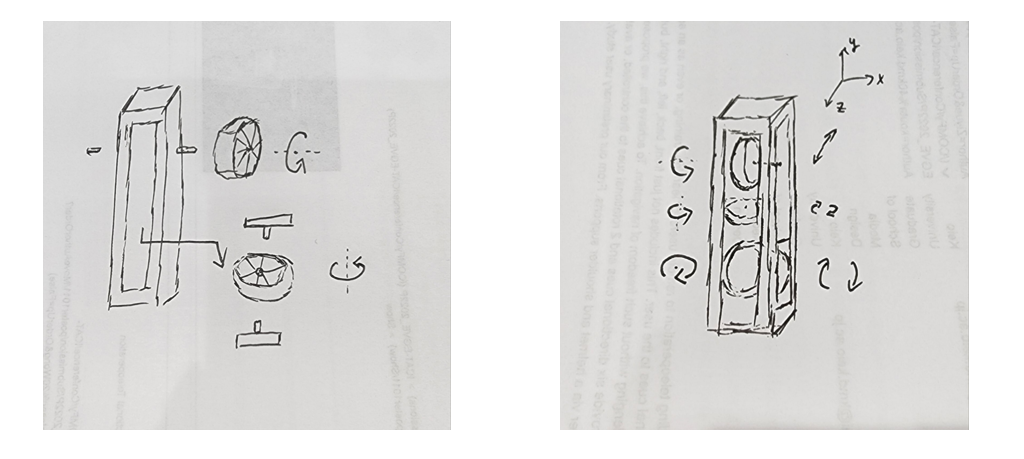
\includegraphics[width=0.8\textwidth]{A_thesis/figures/027.png}
\caption{Design drafts for design 1}
\end{figure}

Design 2:
Placing a vibrator in each direction of the device, using the vibration information of the vibrator to represent different motion states of the object (in the figure, the yellow cylinder represents a vibrator, and the blue represents the support structure).

\begin{figure}[h]
\centering
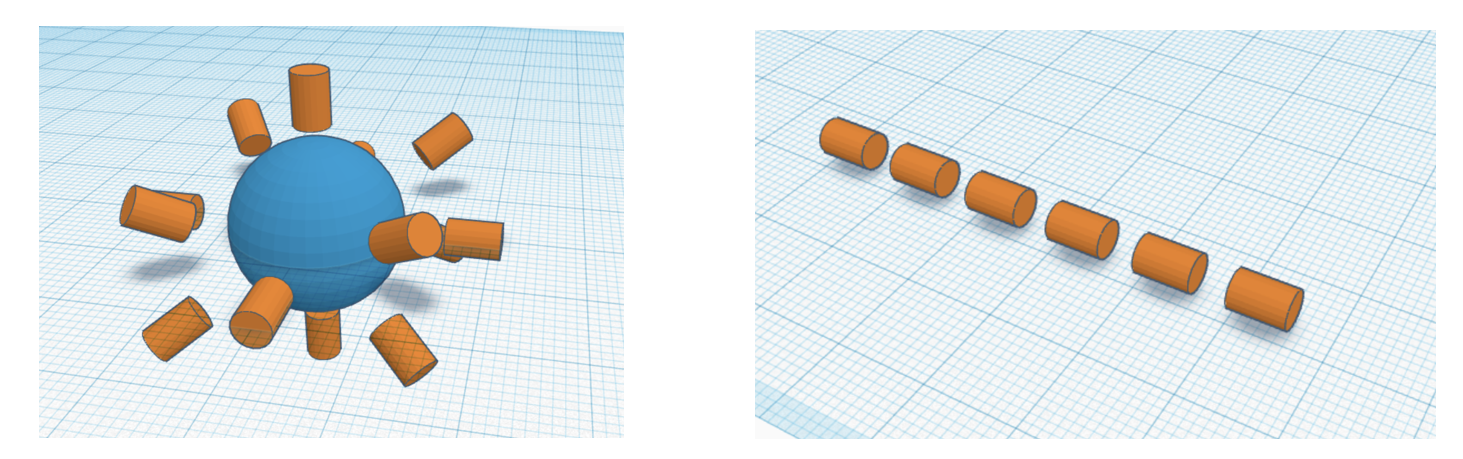
\includegraphics[width=0.8\textwidth]{A_thesis/figures/028.png}
\caption{Design drafts for design 2}
\end{figure}


After subsequent discussions, the first scheme was chosen, that is, using the forward and backward rotation of the wheel to represent the forward or backward movement of the object in virtual space.And at the beginning of the attempts, will focus on exploring the dimension of 1 degree of freedom (1dof). This will build upon our previous attempts, gradually advancing our design and development efforts towards more complex 3 degrees of freedom (3dof) devices.

\subsection{Implement}
\subsubsection{Haptic Design}
In terms of implementation, an Arduino 360 servo was used as the final kinematic performance device. A 3D printed shell was installed on the top of the servo, and it was hoped that users could feel the same motion situation in the virtual space by feeling the rotation of the external touch lid.
Furthermore, the push-pull structure of the crank was tried, and a shell was placed on the user's hand. The internal flat structure combination was used to express the advance and retreat of the object by means of thrust and pull. However, the kinematic performance was significantly weaker than the wheel structure.
In terms of system control, Unity and Arduino were used for serial communication, using Unity to transfer parameters to adjust the digital output signal of Arduino to control the servo. Users can control the rotation of the server by controlling the direction key.

\begin{figure}[h]
\centering
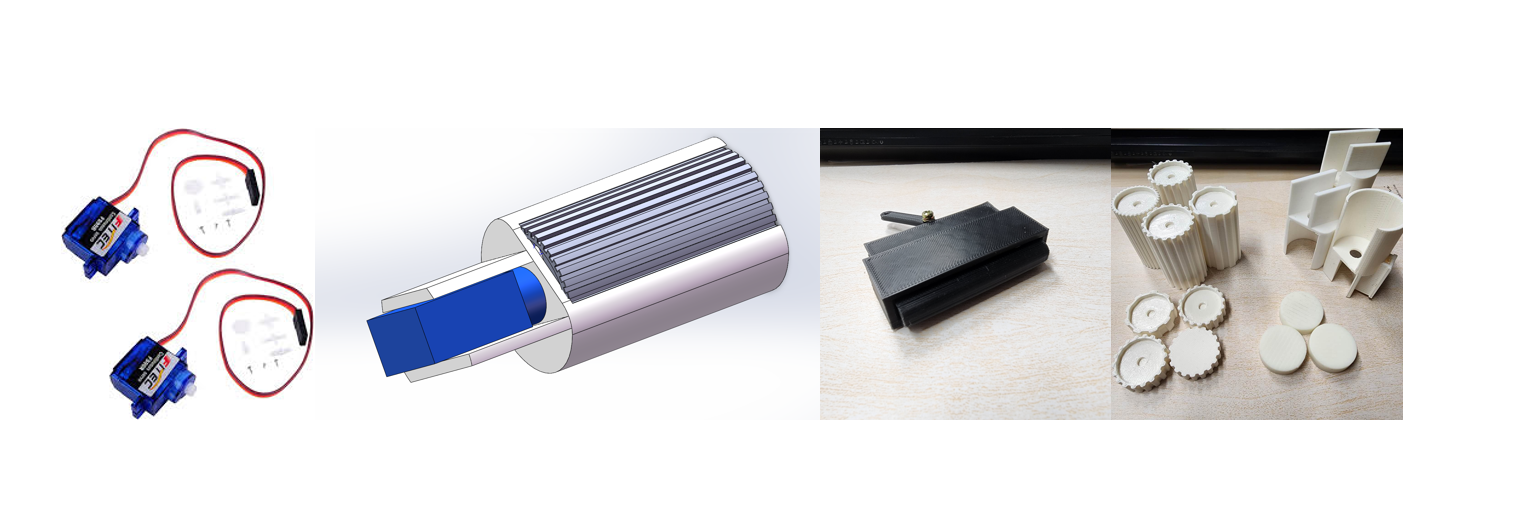
\includegraphics[width=0.9\textwidth]{A_thesis/figures/029.png}
\caption{Research process (3650 servo, 3d design, crank design, 3d printing)}
\end{figure}

\subsubsection{3D Print}
Using the 3D printed structure, the part that the user touches and the rotating part of the servo were separated. Depending on the different parts of contact, the kinematic effects produced are also different. For example, in the internal tests, the moving servo parts responsible for the forward and backward movement direction have weaker haptic effects than those interacting with the user's fingertips because they mainly contact the inside of the hand (including the inside of the fingers and the palm). The texture of the contacted object's surface also has different effects on the kinematic expression. For instance, a surface with a concave and convex texture can produce stronger haptics than a smooth surface, but too many bumps may cause pain during use. Therefore, after tests, a moderate concave and convex surface was chosen to ensure effective haptics without causing pain to the user during use.
In addition, according to the tests, the kinematic effect provided by the rotating movement varies depending on the relationship between the rotating contact area and the position of the palm. The kinematic performance when the rotation axis is parallel to the palm surface is significantly weaker than when they are cross-vertical. Based on the above tests and adjustments, the final choice was to increase the contact area to improve the user's experience.

\subsubsection{System Design}
In system construction, Unity was not only used as the main control interaction interface but also for building a visual prompt application scenario for users. A simulated driving system was set up in Unity. In such an application scenario, users can control the movement of the car in the scene to synchronously rotate the servo in the handheld device.

\begin{figure}[h]
\centering
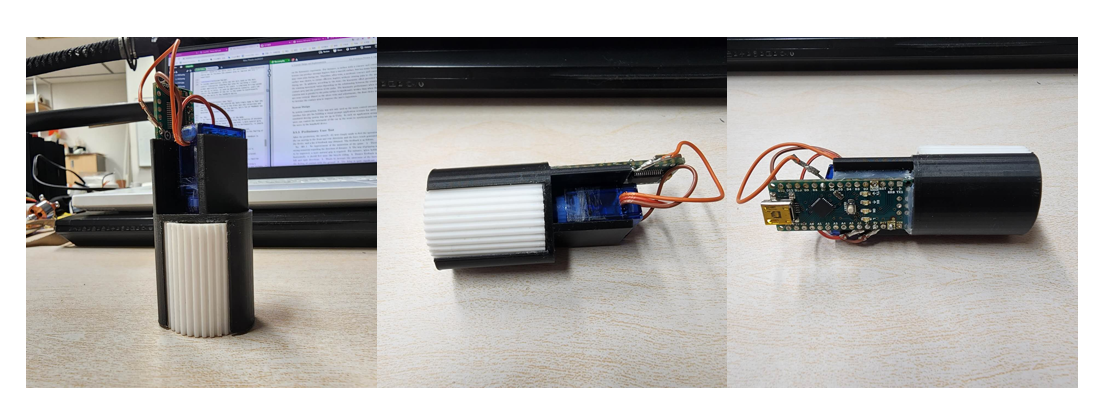
\includegraphics[width=0.9\textwidth]{A_thesis/figures/030.png}
\caption{Three views of the prototype}
\end{figure}


\subsection{Preliminary User Test}
After the production, the users(N =6) were simply made to feel the operation of the car moving in the front and rear directions and the force touch generated by the device, and a lot of feedback was obtained. The feedback is as follows.

No. 001:    1. No improvement of the immersion of the game.
2. There's a strong sensation regarding the direction of distance.
3. The way of gripping needs to be improved, a more natural grip is required. For instance, when holding it horizontally, it should feel more like bicycle riding.
4. Desires feedback in the left and right directions.
5. Wants to increase the awareness of the tires and the feeling of contact with the ground.
6. The delay is quite significant, more immediate feedback is desired.

No. 002:    1. There's a distinct feeling of moving forward.
2. The tactile feeling of moving forward and backward is inconsistent.
3. The contact area with the palm needs to be well planned.
4. Desires a diagonal forward direction.
5. There might be a greater enhancement for visually impaired individuals.
6. When used in a video or racing environment, providing a corresponding sense of speed would be more immersive and increase the distance between the user and the racer.

No. 003:    1. Desires force feedback in the left and right directions.
2. Bugs and delay greatly affect the overall immersive physical experience.
3. The choice of Vection in the forward and backward direction has an impact on the user.
4. The method of grip requires moderate pressure, to avoid being too hard to turn, or too light to feel.
5. Continue fixing bugs.

No. 004:    1. Desires the inertial feeling of stopping when finally parking.
2. Wants the feeling of acceleration pushback.
3. Considering how to integrate with the controller.

No. 005:    1. There's no sense of unity between the controller and the system.
2. Visual impact?
3. The feeling in the two directions is inconsistent.
4. The rotation towards one's own body direction is more intense.

No. 006:    1. The sensation of moving direction is very strong.
2. Holding with one hand and operating with the other creates a serious feeling of disconnection.
3. Wants feedback of the dull feeling when stopping and the vibration of movement.
4. Integration with the joystick? Embedding?

\section{Prototype Version 4 -2dof}
\subsection{Concept Design}
After the previous testing, the system first and foremost presented a very obvious kinematic effect, and the user's physical sensation also successfully approached the research goal, i.e., feeling the moving state of the moving object, including the moving direction and rotation angle. However, there were still some missing details, such as the relationship of velocity vectors. Moreover, due to the application scenario, most users demanded not only the kinematic feedback of the 1dof forward and backward, but also strongly required at least the corresponding kinematic feedback in the left and right directions. Additionally, some aspects of the system needed to be optimized, such as reducing communication latency, decreasing the duration of single rotation, increasing the update detection frequency, and considering other possible application scenarios outside of the device's kinematic effects, such as whether it can enhance the user's connection with the virtual vehicle.

\subsection{Implement}
According to the requirements from the previous user test, the system update mainly provided rotation in the left and right directions. A 360-degree server in the left and right directions was set up in the center of the user's palm, parallel to the user's palm. Due to the natural curve of the human hand during use, the edges of the cover were beveled to avoid pain during use.
Additionally, the system settings changed the third-person perspective to a first-person perspective, better simulating the user's real experience in a driving environment. 

The system is not only in positive correlation with the direction and angle of moving objects in virtual space,  the rotation speed of the device would also change in real time according to the speed of the virtual object. The adjustments in the system also included increasing the refresh rate of the serial communication, raising it from the original refresh rate to the current one, and reducing the duration of a single rotation. This effectively avoided communication backlog in the serial port, where the signal processing time of the first input is too long, leading to the inability of the subsequent input signal to be processed in time.

\subsection{Functional Explanation}

This sections will delineate the functionality and operational methodology of the prototype developed in this research. 

The device consists of two servo motors, referred to as Servo1 and Servo2. 
\begin{figure}[h]
\centering
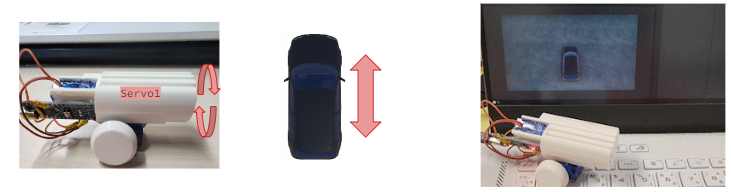
\includegraphics[width=0.9\textwidth]{A_thesis/figures/033.png}
\caption{Illustration of servo1}
\end{figure}
Servo1 is horizontally positioned within the central chamber and interconnected with a rotating wheel. The surface of this wheel makes contact with the user's inner finger. When there is a displacement in the vehicular movement within the virtual environment, either forward or backward, Servo1 initiates a rotational movement. This allows the user to perceive the locomotive state of the virtual vehicle through the friction between their finger and the wheel. Specifically, forward motion in the virtual vehicle prompts a clockwise rotation of the wheel, while a backward motion triggers a counter-clockwise rotation.
\begin{figure}[h]
\centering
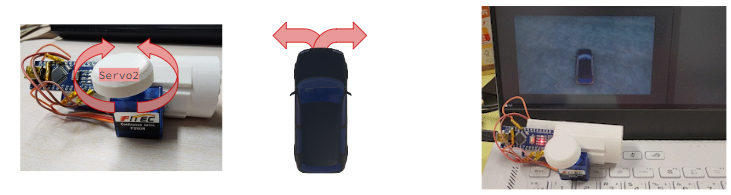
\includegraphics[width=0.9\textwidth]{A_thesis/figures/034.png}
\caption{Illustration of servo2}
\end{figure}
Servo2, placed externally on the device, is linked with a turning wheel, the surface of which interacts with the user's palm center. This arrangement facilitates the conveyance of rotational information concerning the vehicle within the virtual environment to the user via the wheel's movement. When the virtual vehicle pivots either to the left or right, Servo2 responds by rotating in the respective direction. Thus, a leftward rotation of the virtual vehicle results in a leftward wheel movement, while a rightward vehicle rotation induces a rightward wheel movement.

\begin{figure}[h]
\centering
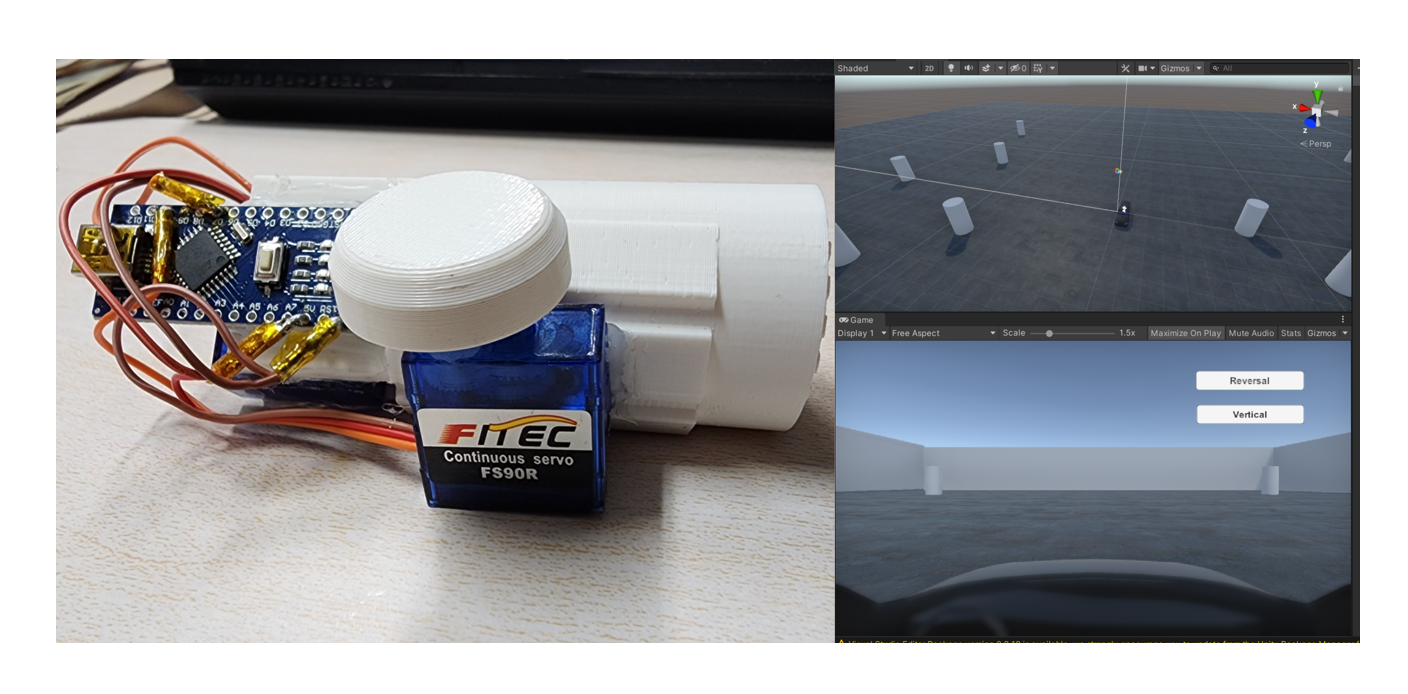
\includegraphics[width=0.9\textwidth]{A_thesis/figures/031.png}
\caption{Final prototype and virtual environment demonstration}
\end{figure}
Concerning the user interaction interface, as depicted in Figure 3.16, a simple virtual vehicular movement scenario has been created using Unity3D. The setting comprises walls, minor mazes, and cylindrical obstructions at randomized locations, simulating a conventional road scenario to approximate the real-world user environment as closely as possible. Users observe from a first-person perspective and can manipulate the vehicle's movement - forward, backward, left, and right - using the directional keys on the keyboard. In tandem with accepting control signals, Unity3D also transmits them to the MotionPerformer via serial communication.


\textbf{For the coding of unity and arduino, please refer to the appendix 'A' and 'B'.}
\chapter{Proof of Concept}
\section{Introduction}
Experiments will be conducted in a quiet studio setting with the MotionPerformer, a laptop, and a monitor. The Each experiment will be with a unique objective, spanning a total duration of 40 minutes.

The objectives for each experiment are as follows:
Experiment 1 validates the effectiveness of this design in mechanically representing object motion information.

Experiment 2 concentrate on the user's holistic experience when utilizing the device within two distinct application scenarios: passive scenario and active scenario. These parts will also compare the user experience with and without the device.

%\section{Usability Measurement}

\section{Experiment 1: Haptic Performance Test}
\subsection{Experiment Description}
The primary hypothesis for Experiment 1 is that “Users can accurately discern the movement status of a virtual vehicle, which includes both displacement (direction, distance), rotation (direction, angle) and speed information." 

This experiment will employ three experimental conditions, which condition will be conducted eight motion tests. This totals 24 sub-tests, all to be completed within a 20-minute time frame.

The experimental conditions are separated into three categories: Only-visual, Only-haptic, Visual-haptic. To mitigate potential errors arising from experiment sequencing, the order of conditions will vary based on the participant's ID number. For odd-numbered participants (1, 3, 5, 7), the sequence is "Only-visual, Only-haptic, Visual-haptic". For even-numbered participants (2, 4, 6, 8), the sequence is "Only-haptic, Only-visual, Visual-haptic".

\begin{figure}[h]
\centering
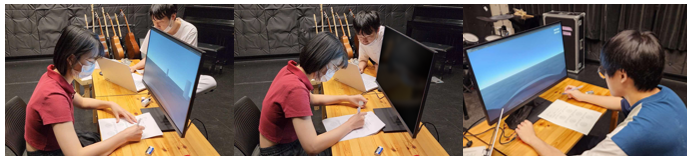
\includegraphics[width=0.8\textwidth]{A_thesis/figures/036.png}
\caption{Three experimental conditions}
\end{figure}

Under Only-visual conditions, participants do not use the MotionPerformer and rely on visual cues to judge and describe the current movement status of the vehicle. Under Only-haptic conditions, participants hold the device and depend entirely on the haptic feedback provided by MotionPerformer to describe the vehicle's current movement state. For Visual-haptic conditions, participants hold the MotionPerformer while watching the monitor, using both visual and haptic to judge the vehicle's movement state.

The motion tests will encompass various movements including fast forward, slow forward, fast backward, slow backward, fast left, slow left, fast right, and slow right. To circumvent participants' inherent directional biases, the sequence of tests will be randomized. The final sequence is slow left turn, fast left turn, fast forward, slow backward, fast backward, slow right turn, slow forward, and fast right turn. After each test, the vehicle returns to its initial state, ensuring that the next test does not build upon the prior one's movement state. Each test involves a single type of motion, such as a left turn or a forward movement, and compound movements are not included in the tests. Unless otherwise required, each test is conducted only once.

The motion detection method draws inspiration from \cite{paper36}, using drawing as a mode of testing. Staff input commands via keyboard, and participants, upon feeling the device's operations, will depict each motion's status graphically. The central black area in the figure signifies the position of the virtual vehicle/avatar, and each chart should indicate both the direction of displacement (forward or backward) or rotation angle (left or right) and the perceived speed, represented by the thickness of the pen line.

\subsection{Experiment Preparations}
Before the experiment, participants will be introduced to the fundamental information about the device and system and its operation, followed by a swift test to ascertain their preferred mode of operation. As documented in \cite{ref_motion001}, participants exhibit two primary patterns of perceiving movement direction: the device's motion either aligns or contrasts with the actual direction of movement, with both preferences appearing with equal probability. Consequently, it's crucial to explain the correlation between the device's movement data and the physical object's movement data to the participants before starting the formal testing.

Also, from earlier pilot tests, we learned that the device might pinch the user's hand, potentially affecting their assessment. Therefore, participants are advised to adjust their grip to a comfortable state where they can perceive the mechanical feedback but not impede the device's normal functioning. Each test will be performed once per session, barring any special requirements.

\subsection{Experiment Procedure}
Upon completion of preparations, participants will conduct three rounds of testing, including "Only-visual", "Only-haptic" and "Visual-haptic". Each round of testing consists of eight sub-tests, followed by filling out the questionnaire.
\begin{figure}[h]
\centering
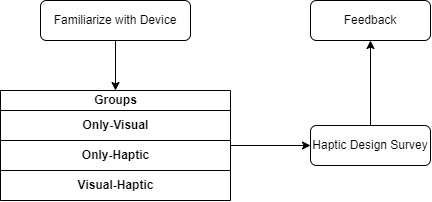
\includegraphics[width=0.7\textwidth]{A_thesis/figures/037.png}
\caption{Flowchart of Experiment 1}
\end{figure}

At the end of Experiment 1, participants will be asked to indicate on the subsequent graphic the haptic sensations they experienced in their palms. These inputs will serve as valuable recommendations for future design modifications and feedback on the overall device performance and user experience.

\begin{figure}[h]
\centering
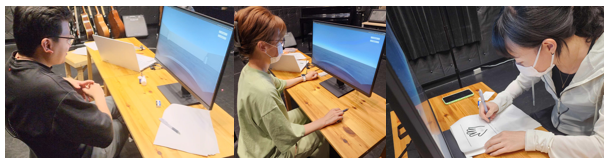
\includegraphics[width=0.8\textwidth]{A_thesis/figures/038.png}
\caption{Photos during Experiment 1}
\end{figure}

\textbf{For further details on the experimental questionnaire, please refer to the appendix 'C'.}

\subsection{Results}
\subsubsection{Motion Information Diagram}
\begin{figure}[h]
\centering
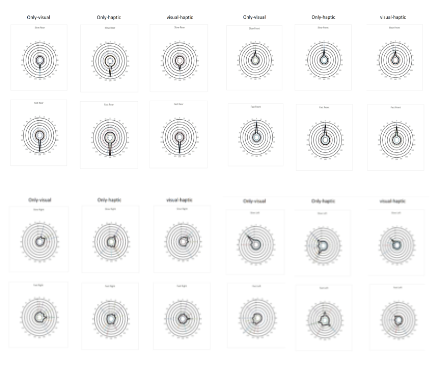
\includegraphics[width=0.5\textwidth]{A_thesis/figures/039.png}
\caption{Results of motion information diagram}
\end{figure}

\textbf{Please refer to the appendix 'E'.}


\subsubsection{Haptic Sensation of Hand}

\begin{figure}[h]
\centering
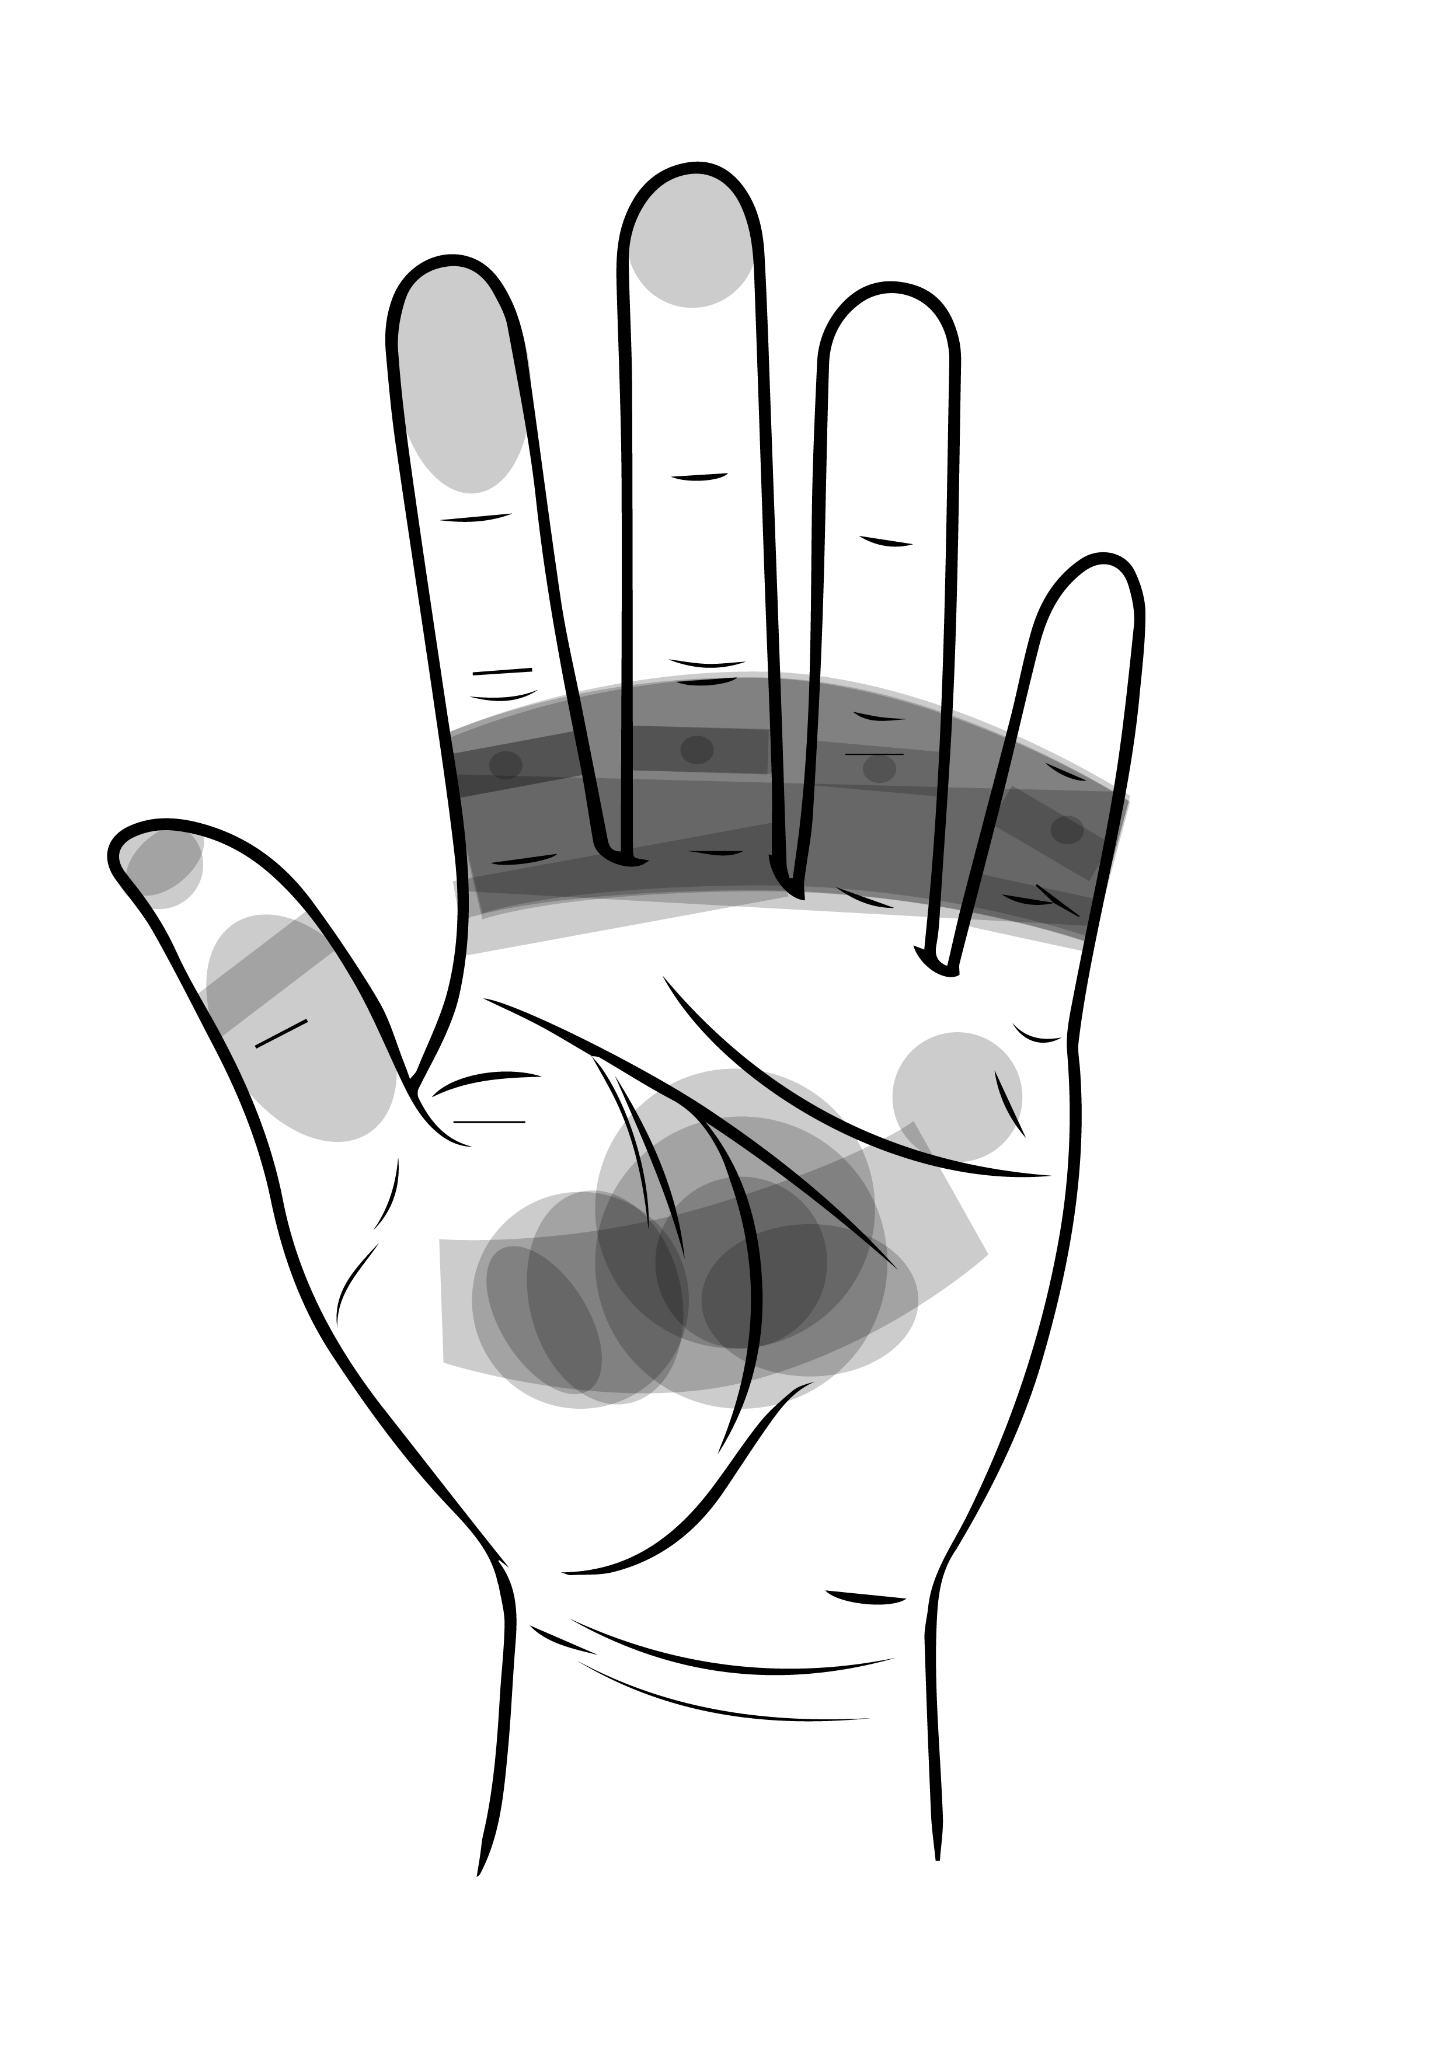
\includegraphics[width=0.3\textwidth]{A_thesis/figures/016.png}
\caption{Results of the hand diagram}
\end{figure}



\subsubsection{Feedback Recording}
001: "I think having haptic feedback in games or while driving would be quite magical. However, the feeling of moving forward and backward is more intense than turning."

002: "Haptic can provide me the intensity of movement which is something that only-visual cannot provide. But only-haptic cannot precisely provide me the information of the distance moved. So, the combination of haptic and visual can provide the best experience."

003: "My hand got a bit pinched."

004: "Everything felt faster and farther when haptic was involved, especially in the mixed condition while the visual didn’t feel that fast/far, the haptic felt very fast and far."

005: "After using the device, the physical reference became easier to grasp, and the experience became more intense."

006: "Haptic touch gave me a stronger feeling when the car moves than visual."

007: "Visual haptic is much better for the experience. The haptic device is good for sensing speed."

008: ”The feeling from haptic is strong, I can easily tell direction and angle, but not so much for speed changing. Haptic on palm is good, can keep fingers free for other things. When seeing and feeling at same time, I look at vision first but haptic feels faster.”

009: “Speed of vision and haptic not same, in experiment design, setting reference for haptic and vision speed first can help a lot in understanding later experiments.”

010: "When using only visual, it's difficult to perceive the angle. Only-haptic needs time to respond to left and right judgements."


\section{Experiment 2: User Experience Test}
\subsection{Experiment Description}
The purpose of Experiment 2 is to evaluate the integrated user experience of using the MotionPerformer in simulated scenarios. This experiment is divided into two rounds of testing according to usage scenarios: the first round involves passive scenario testing, and the second round involves active scenario testing.

In the passive scenario, we employ the Wizard-of-Oz method\cite{paper37}, where staff will simulate the operation of the vehicle's motion in a virtual space by an AI system in the driving system. Users are required only to receive the vehicle's motion information through a display or the MotionPerformer.

In the active scenario, users themselves are required to control the vehicle's movement, while simultaneously receiving the vehicle's motion information via a display or the MotionPerformer.

Moreover, within each round of testing, we adopt the within/without method. This approach facilitates the comparative testing of user's overall experience of the MotionPerformer when receiving both visual and haptic motion information via a display and the MotionPerformer, against scenarios when they are only receiving visual motion information through a display without using the MotionPerformer. 
And to avoid bias, odd-numbered participants will undertake the 'within' test first, followed by the 'without' test. Conversely, even-numbered participants will undertake the 'without' test and proceeding to the 'within' test.

Upon the conclusion of each experiment, they will be requested to fill out a relevant survey questionnaire.The questionnaire for this experiment is composed of two parts. The first eight options stem from the experiment and survey on the sense of agency \cite{paper38} . The final eight options are informed by a user experience survey within a gaming context\cite{paper39}.

\subsection{Experiment Procedure}

\begin{figure}[h]
\centering
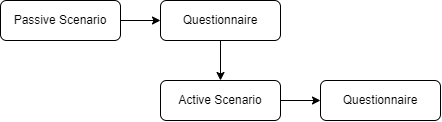
\includegraphics[width=0.8\textwidth]{A_thesis/figures/042.png}
\caption{Flowchart of Experiment 2}
\end{figure}

Upon completion of Experiment 1, and after briefly introducing the procedure of Experiment 2 to the participants, Experiment 2 will commence directly. Participants will first undertake the initial round of testing in passive usage scenarios simulating AI driving. The virtual vehicle will operate automatically, requiring no active manipulation by the participants, who will experience the motion state of the virtual vehicle through the screen and the MotionPerformer. This includes two sub-tests under both 'within' and 'without' conditions. Each sub-test will last for one minute, followed by a requirement for participants to complete the questionnaire.

After the conclusion of the two sub-tests in the first round, the second round of active usage scenario test will begin. In this phase, participants will actively control the motion of the vehicle using the arrow keys on the keyboard while experiencing the motion state of the virtual vehicle through the screen and MotionPerformer. This round also includes 'within' and 'without' tests, each lasting for one minute, followed by the completion of the questionnaire.

\textbf{For further details on the experimental questionnaire, please refer to the appendix 'D'.}

\begin{figure}[h]
\centering
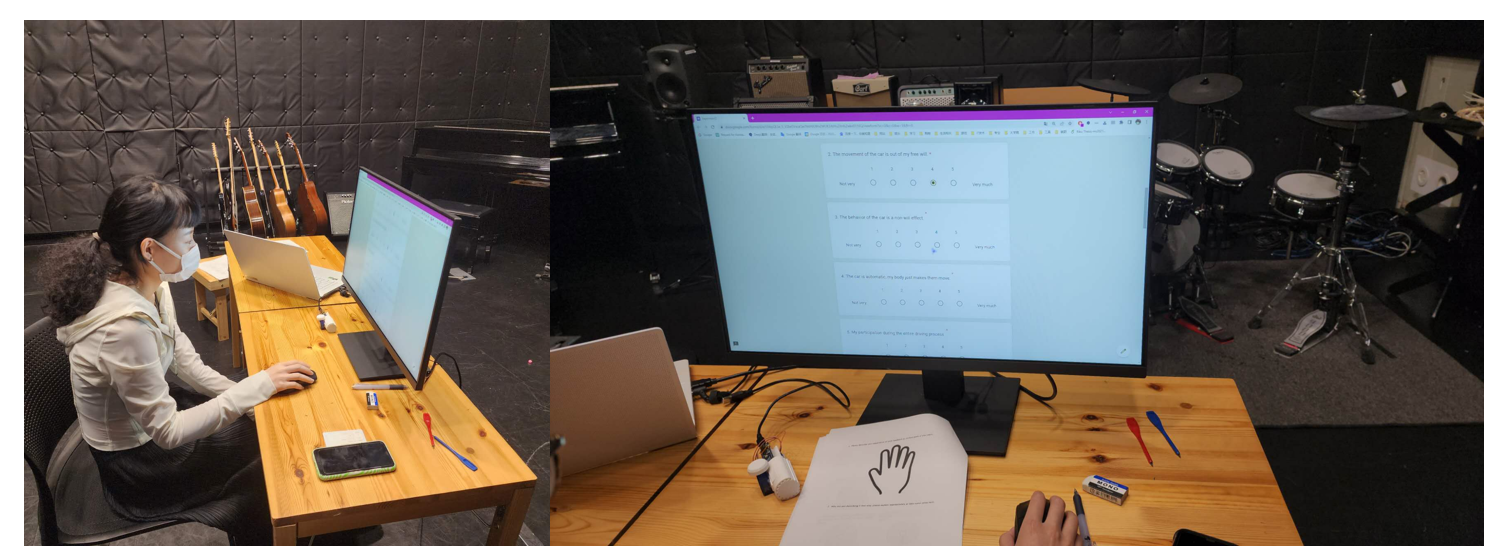
\includegraphics[width=0.8\textwidth]{A_thesis/figures/018.png}
\caption{Photos of the experiment2}
\end{figure}

\subsection{Results}
\begin{figure}[h]
\centering
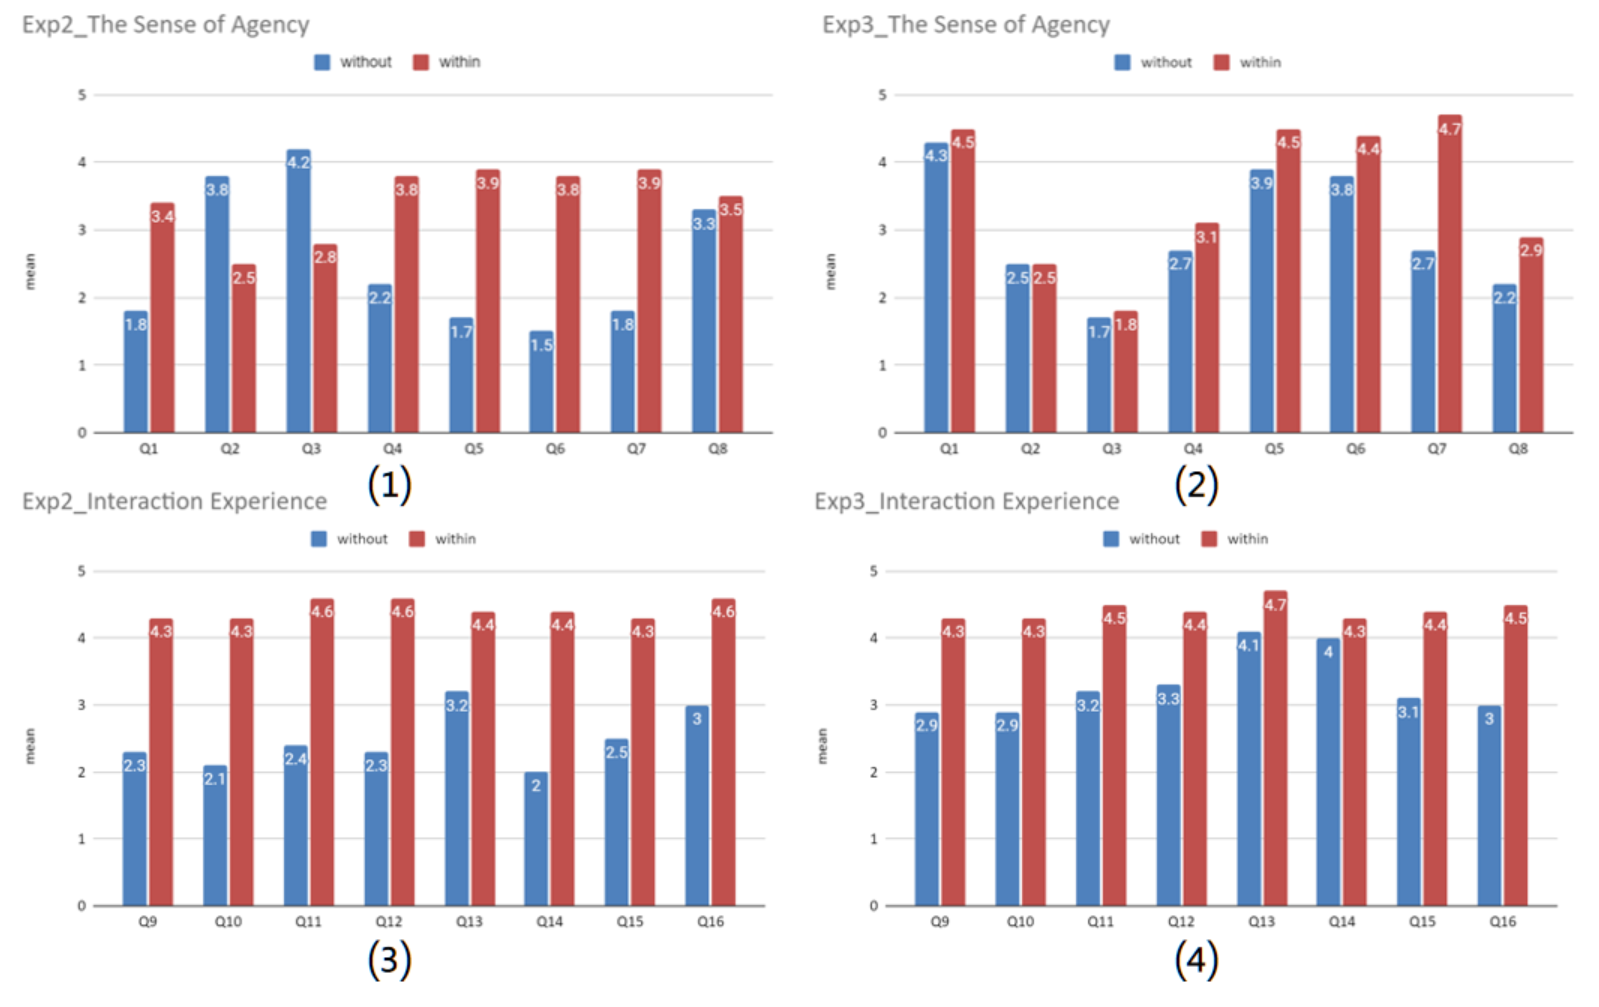
\includegraphics[width=0.8\textwidth]{A_thesis/figures/043.png}
\caption{Data visualization of experiment 2 results}
\end{figure}

After collecting all the data, we visualized in the form of bar graphs. According to the direction of the questionnaire and the different usage scenarios, the data is presented in four different charts, as seen in Figure 4.8: (1) the sense of agency in passive scenarios, (2) the sense of agency in active scenarios, (3) the sense of interaction in passive scenarios, and (4) the sense of interaction in active scenarios. Within these charts, the 'with' and 'without' experiment conditions are differentiated using blue and red respectively. Blue represents the experiment results without using the MotionPerformer, and red represents the experiment results with the use of the MotionPerformer.

On the whole, it can be roughly observed that the use of the MotionPerformer enhances the user's sense of agency and interaction in driving, with some elements even showing a quite significant improvement. A more detailed and specific analysis of the experiment results will be presented in the next chapter.

\textbf{For more data sources data, please refer to the appendix 'F'.}




\chapter{Discussion}

\section{Haptic Performance}
\subsection{From Diagram}
\subsubsection{Motion information}
It is not difficult to discern from the final results that the MotionPerformer system is capable of accurately conveying the direction of movement to users.

In general, individual differences under the 'only-visual' experimental condition are quite minimal. However, in the 'only-haptic' situation, despite having a completely identical system and providing the same haptic feedback for each participant every time, the variances among individuals in response to haptic feedback are noticeably larger than the differences when users obtain movement information visually.

And we will analyze the experimental results from three perspectives - forward and backward displacement movements, left and right rotational movements.

\begin{figure}[h]
\centering
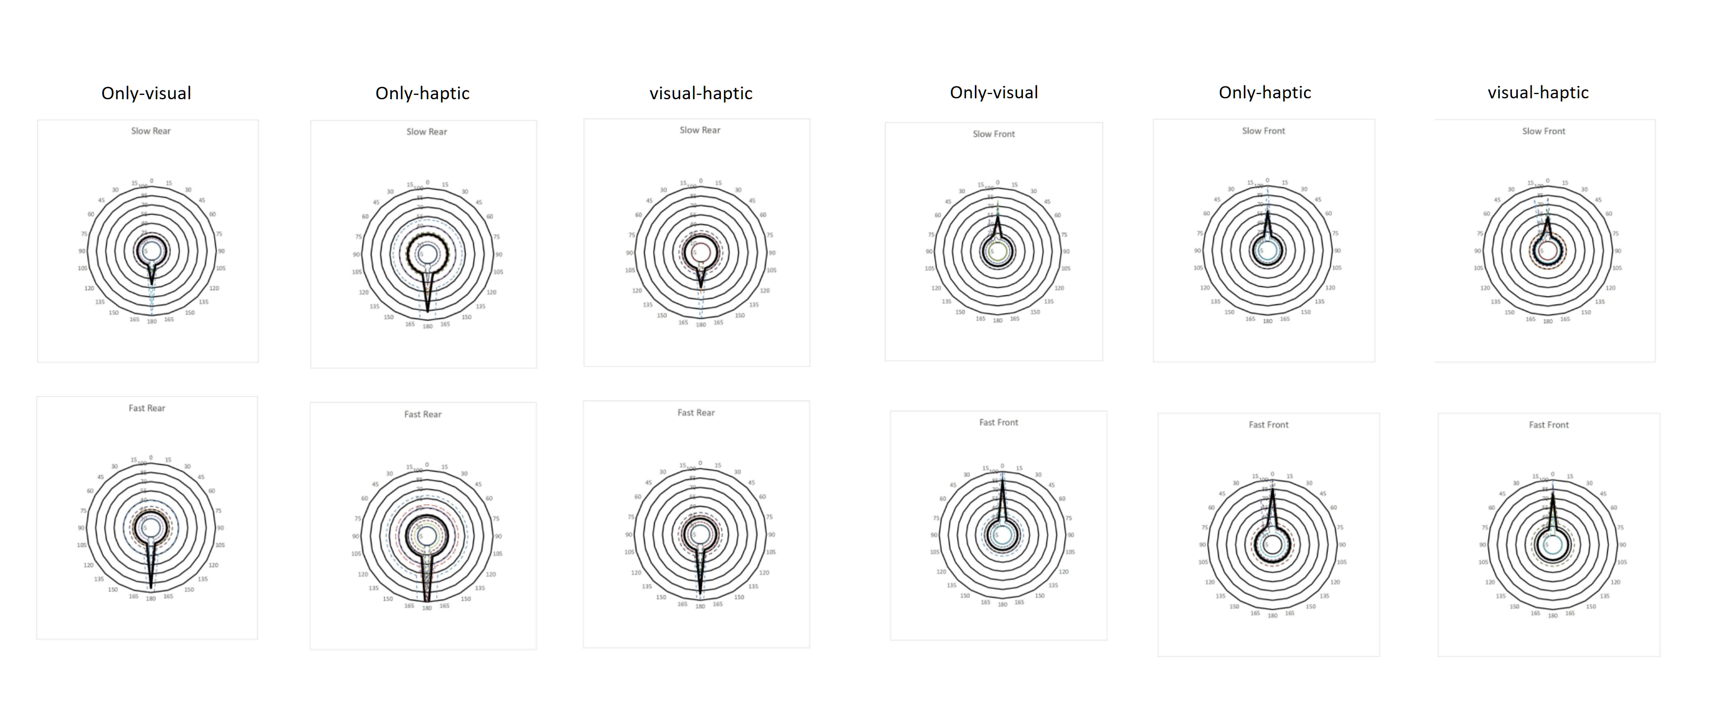
\includegraphics[width=0.8\textwidth]{A_thesis/figures/FrontandRear.png}
\caption{Comparison of displacement direction}
\end{figure}

\newpage
Regarding \textbf{forward and backward displacement movements}, the experimental results under the three different conditions for these two modes of movement are relatively consistent. Notably, user consistency in forward displacement movements is higher than in backward displacement movements. In the backward displacement mode, under the 'only-haptic' condition, users' judgment on displacement distance is significantly greater than in the 'only-visual' condition. Moreover, the judgment variation in high-speed mode is more significant than in low-speed mode, indicating that as speed increases, the perception of backward displacement changes through haptic feedback also intensifies. However, in the combined judgment scenario, the results tend to align more closely with visual judgment.

As for the perception of displacement speed, under the same speed conditions, the speed judged in the 'only-haptic' condition is greater than in the 'only-visual' condition. Yet, in contrast to displacement distance, the rate of increase in speed perception between the low-speed and high-speed modes is nearly the same, with no noticeable difference. After introducing the 'visual-haptic' condition, although the overall trend is the same as the first two situations ('only-visual', 'only-haptic'), it is closer to the 'only-visual' condition compared to 'only-haptic'. Importantly, even though adding haptic feedback results in limited enhancement in displacement variation, it significantly enhances speed perception.

In the comprehensive analysis of displacement direction information, the combined judgment results for forward movement are closer to 'only-visual', while the combined judgment results for backward movement change significantly after introducing haptic feedback. This suggests that incorporating haptic feedback can strengthen users' perception of backward movement. We hypothesize this phenomenon may occur because, in daily life, we experience scenarios involving forward movement far more than backward movement. Furthermore, since the visual direction is always forward, judgments about backward movements require inference from changes in surrounding conditions, making forward movement judgments potentially simpler than those for backward movement. Therefore, our ability to judge forward movement is stronger and more reliant on visual cues. However, the addition of haptic information can enhance our judgment in perceiving backward movement.

\begin{figure}[h]
\centering
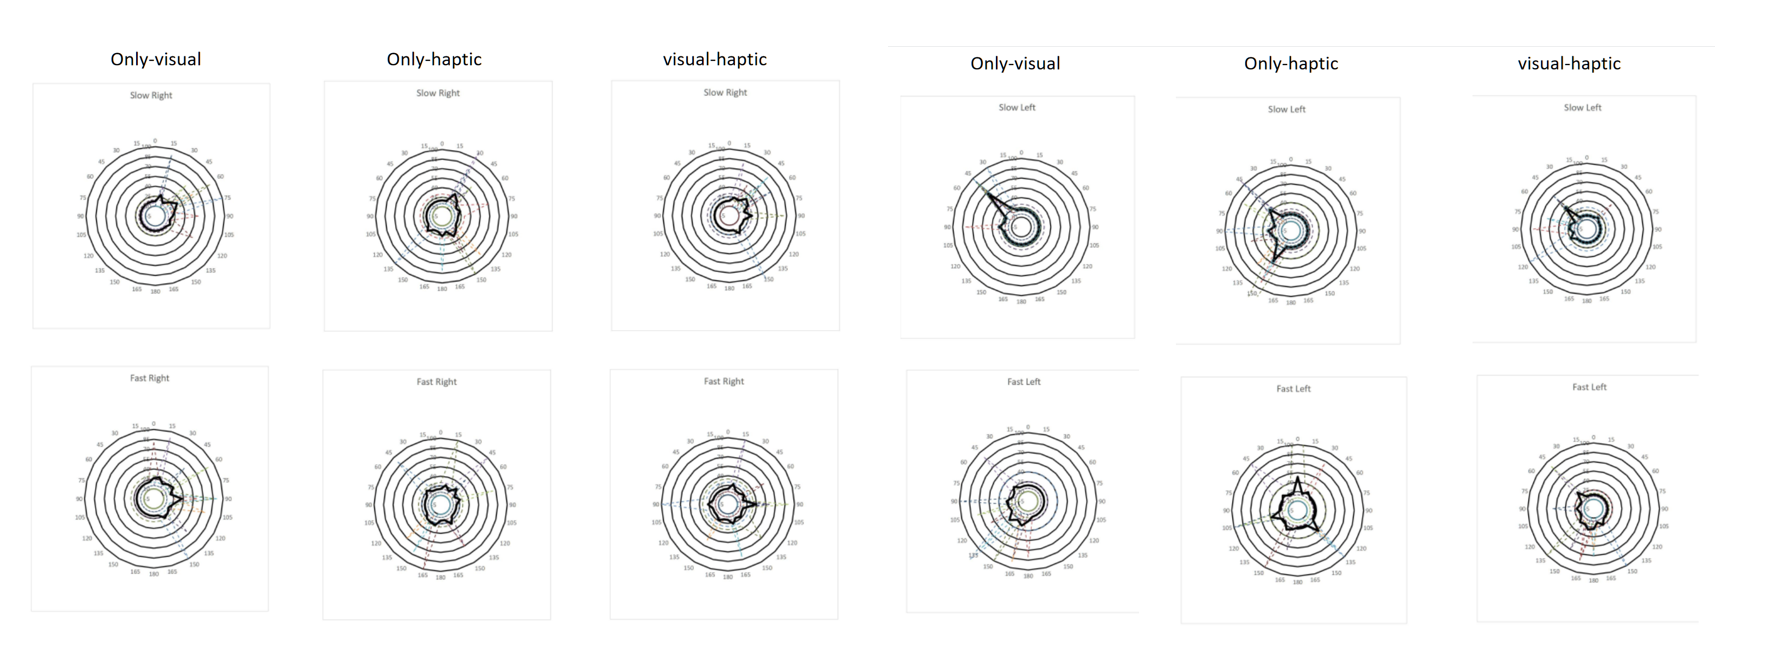
\includegraphics[width=0.8\textwidth]{A_thesis/figures/LeftandRight.png}
\caption{Comparison of rotation direction}
\end{figure}

In terms of left and right rotation, experimental results indicate that haptic feedback significantly enhances users' judgment of rotational angles, but no noticeable improvement is observed in the perception of rotational speed.

For the direction of left-right rotation, the 'only-visual' results are quite concentrated and more accurately represent the actual change in angle. In the 'only-haptic' condition, users' perception of the rotation angle is almost double that of visual judgment. This discrepancy increases in high-speed rotation, to the point that during the experiment, users are unable to discern whether a rotation exceeds 360°. These results suggest that haptic feedback greatly enhances users' perception of changes in rotation angle. However, the specific degree of enhancement cannot be guaranteed by the current results. This is because the rotation speed of the experimental equipment does not accurately correspond to the actual rotation speed, preventing users from establishing their own frame of reference for rotation information in the 'only-haptic' condition. Even in the 'visual-haptic' experimental condition, the introduction of haptic feedback influences users' overall judgment of rotation, reinforcing the aforementioned point. Yet, in terms of rotation angle, the results still align closely with the 'only-visual' condition. This suggests that when significant discrepancies arise between visual and haptic judgments, users still predominantly rely on visual information.

Concerning changes in rotation speed, the introduction of haptic feedback does not noticeably improve speed perception. In the preliminary experiments, users were unable to describe the rotation vector due to excessive speed variation, leading to smaller speed variation ranges in the present experiment. This may be one reason for the lack of significant changes in users' speed perception. Thus, the current experiment's results do not provide a reliable reference for haptic feedback's influence on rotation speed.

Interestingly, the combined judgment after adding haptic feedback is smaller than that of 'only-visual' and 'only-haptic', particularly noticeable in left turns. This indicates that when users receive both visual and haptic information about rotation, their judgment of rotation speed tends to be conservative. However, in the right turn experiment results, introducing haptic feedback did not significantly influence changes in rotation speed. This suggests inconsistent judgment standards when determining left or right rotations.

In summary, regardless of the experimental condition, users judge left turns more accurately than right turns. Even under 'only-visual' conditions, users' judgments of left turns are more focused and precise. This is consistent with the aforementioned point that the judgment conditions or abilities for left and right turns are different, but the specific influencing factors and limitations are not the focus of the current study.

As observed from the results of Experiment 1 Motion Information Diagram, the MotionPerformer can accurately convey the direction of motion to users. Users can perceive speed changes significantly, but the precision of rotation angle information needs improvement. In terms of speed and displacement information, the system can help establish comparisons under different parameters. In other words, the MotionPerformer can provide a reference for mechanics in virtual space, but this reference system is highly subjective. Whether a public, objective mechanical reference coordinate system can be established using the MotionPerformer warrants further consideration and research. Moreover, the MotionPerformer can enhance users' perception of motion information, particularly in backward displacement direction and rightward rotation direction.

\subsubsection{Haptic Sensation of Hand}
During the experiment, users were not forcibly dictated on how to grasp the device. Instead, they were advised to choose a suitable position to minimize the chance of their hands being pinched by the roller part while still being able to feel the haptic feedback.

According to users' descriptions of the areas of their hands that received haptic feedback, which were then visualized and overlapped, results are as follows.

\begin{figure}[h]
\centering
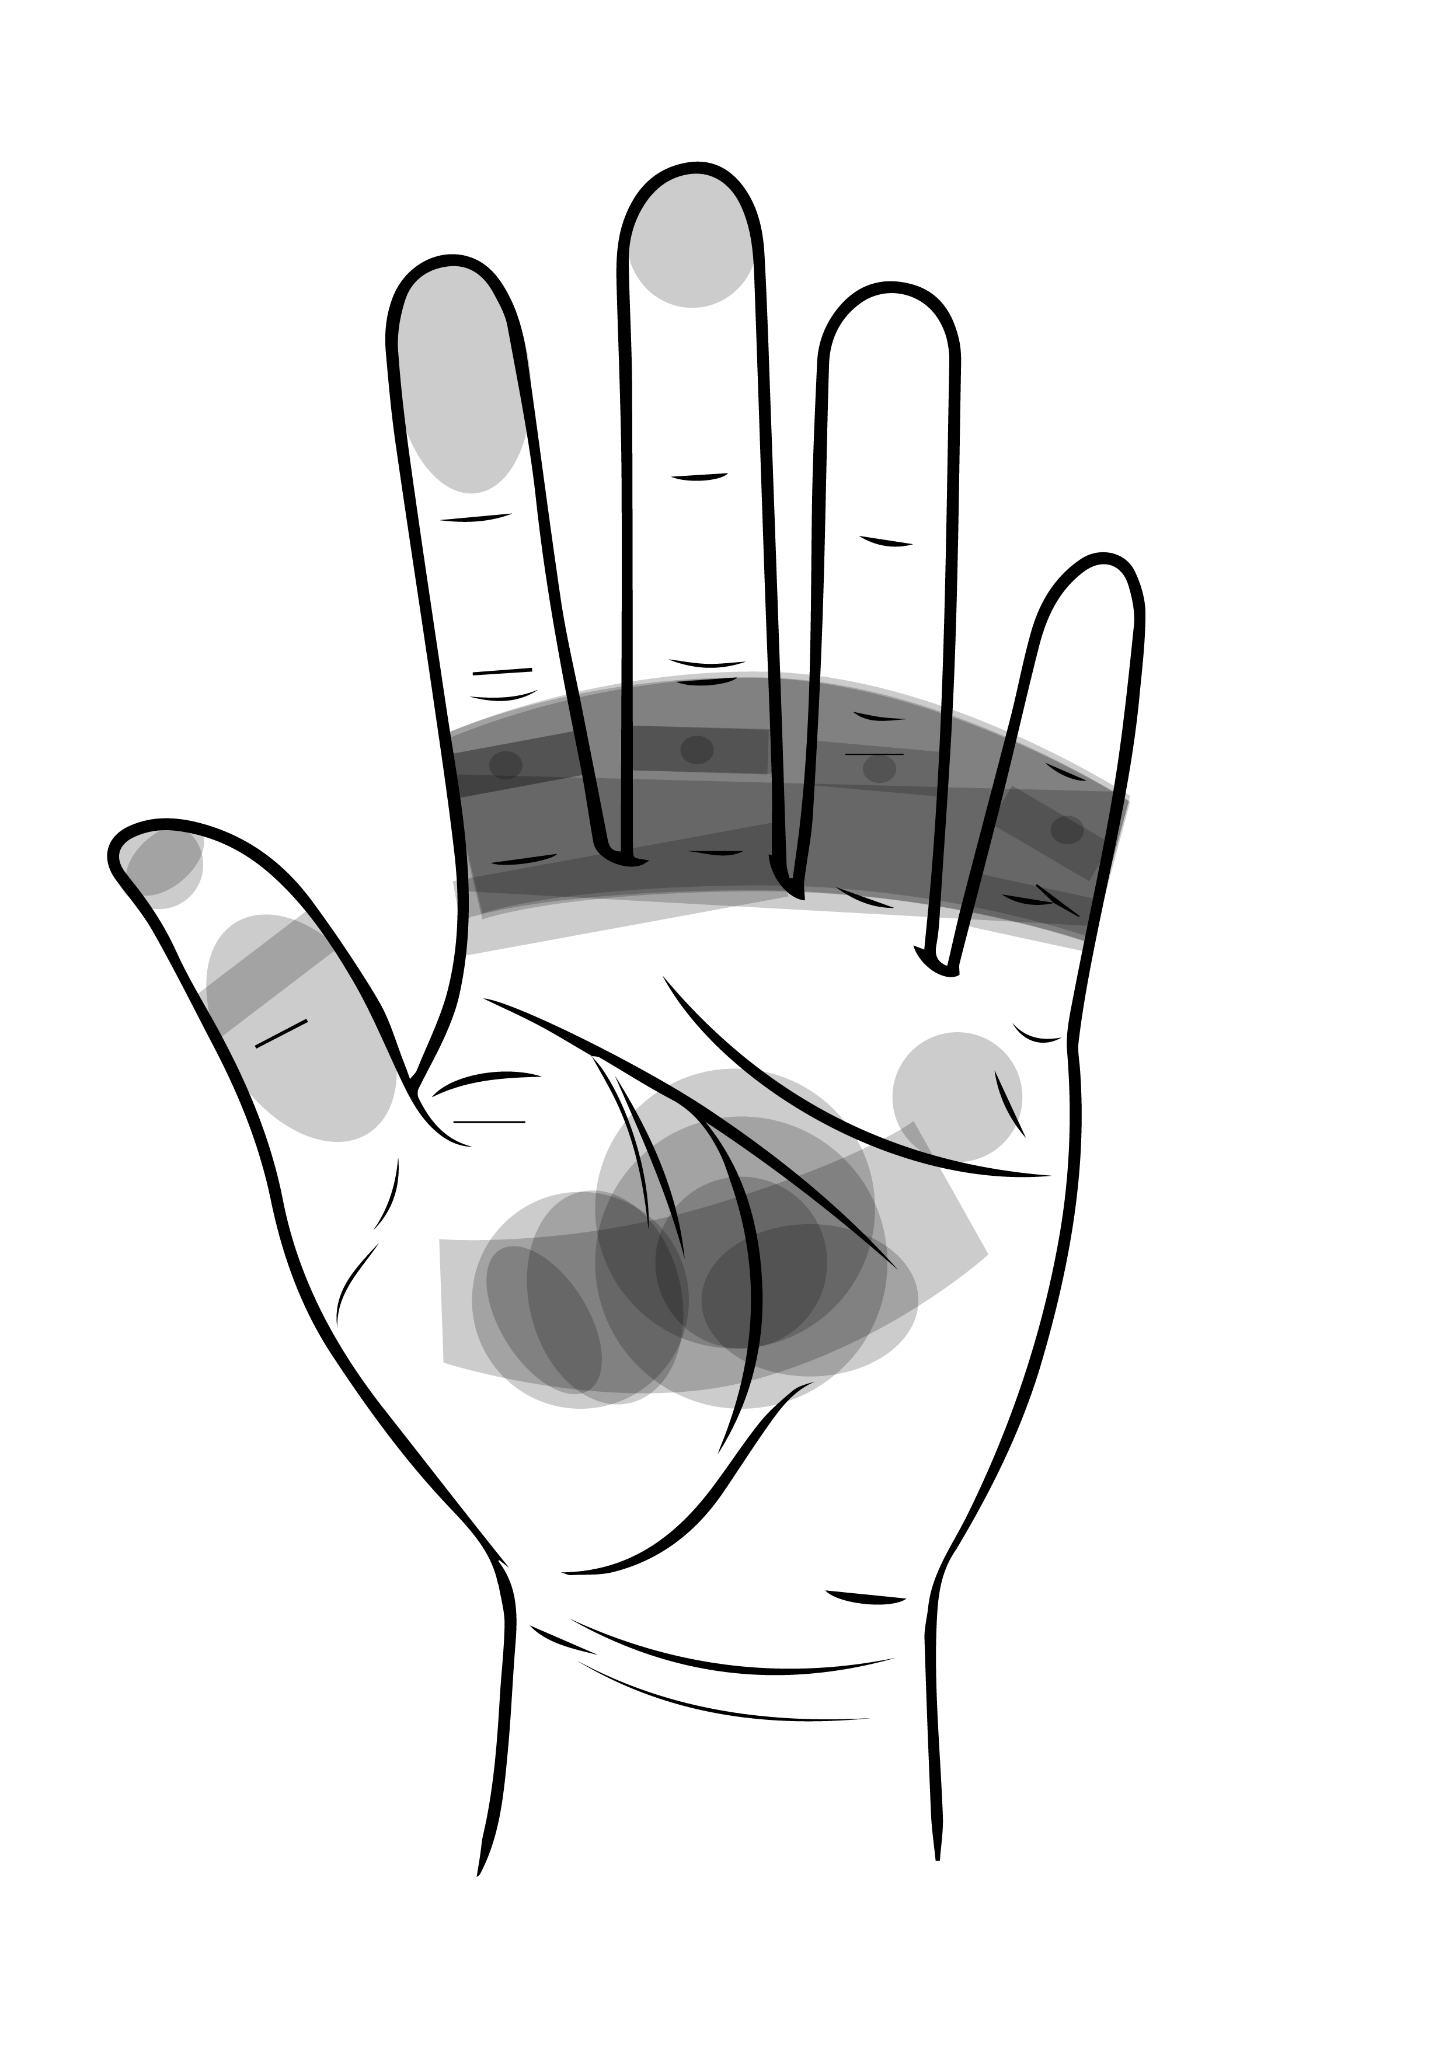
\includegraphics[width=0.5\textwidth]{A_thesis/figures/016.png}
\caption{Results of the hand diagram}
\end{figure}

As the design concept, users primarily felt haptic feedback in areas depending on how they gripped the device, mainly on the back of the third joint of their fingers and a slightly lower position at the center of their palms. 

Interestingly, the index finger had a larger area of haptic feedback compared to other fingers. This isn't just because the index finger is used more often in our daily lives, but also because the natural grasp of the hand is not a horizontal cylinder. Instead, it is a grip where the tail end (little finger) slightly points downward. This point should be taken into consideration in future designs, as a more natural grip could potentially reduce incidents of pinching and enhance the user experience.

In the palm area, the most haptic feedback was not in the center, but mainly in the regions of the flexor digiti minimi brevis muscle (which flexes the little finger) and the flexor pollicis brevis muscle (which flexes the thumb). The reason is similar to what was mentioned earlier. In the natural grip posture, these two areas make contact with the MotionPerformer at certain angles. The haptic feedback provided by these two areas is stronger than the haptic feedback directly received at the center of the palm where it makes contact with the MotionPerformer.

\subsection{From Feedback}
Further evidence supporting the conclusions drawn earlier can be found in users' feedback.

Firstly, users positively affirmed the haptic sensation for directional and angular changes. According to the feedback, users reported a stronger perception of directional vectors compared to rotation vectors through haptic feedback (001). Similarly, the haptic perception of speed information was also found to be more intense than visual perception (002, 007). Although vision can provide more accurate information (002), haptic information proves to be a better judge in certain situations where visual feedback is insufficient, such as during rotation (010).

In comprehensive use scenarios, when both visual and haptic feedback convey the same motion information, users tend to rely more on visual information. However, in situations where visual information is abundant, haptics can provide instant feedback about changes (009), a feature where it distinctly outperforms vision. Several participants also mentioned that adding haptic feedback to the perception system, through the collaboration of vision and haptics, enhances users' overall perception of moving objects in virtual space (002, 004, 008). This allows for a better user experience and a more realistic feeling (001, 005). Generally, the significance of adding the haptic device, MotionPerformer, lies in aiding users to establish a mechanical haptic reference for the self-moving objects in virtual space (005).

Lastly, regarding the reliability of the device, even after optimization, some users still made suggestions for improvements. For example, device latency and judder were mentioned as factors that could reduce immersion during use (004). Incidents of hand pinching were also brought up sometime (003). During testing, it was noticed that pinching incidents occurred more frequently among female testers. Therefore, improvements in device reliability and design are needed in future iterations to achieve a better user experience. Moreover, in terms of experimental design, helping testers establish a reference relationship between vision and haptics prior to the formal test could significantly improve users' perception of accuracy in subsequent processes (008).

\section{User Experience}
\subsection{The Sense of Agency}
In the first eight questions of the questionnaire, the main content was to test whether the device possesses a sense of agency. Four questions (Q1, Q5, Q6, Q7) have a positive impact on the sense of agency, the higher the value, the stronger the sense of agency. The other four questions (Q2, Q3, Q4, Q8) negatively impact the sense of agency, the higher the value, the weaker the sense of agency.

In the analysis process, the Cohen’s d value was calculated to assess the effectiveness of the difference between the two situations in addition to the use of t test for the calculation of statistical differences. The following discussion is arranged from the largest to smallest Cohen's d value.

\begin{figure}[h]
\centering
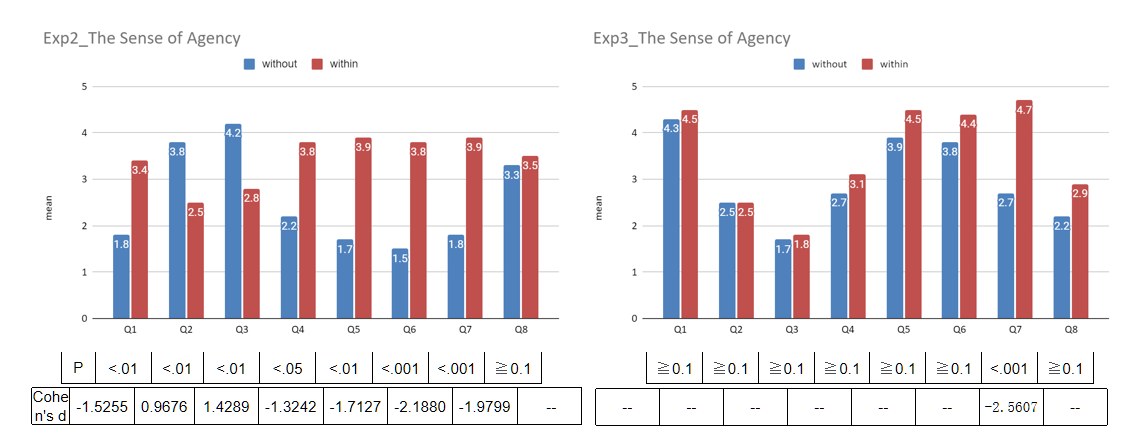
\includegraphics[width=0.9\textwidth]{A_thesis/figures/040.png}
\caption{Data visualization on the sense of agency}
\end{figure}

\subsubsection{Passive Usage Scenarios}
\begin{figure}[h]
\centering
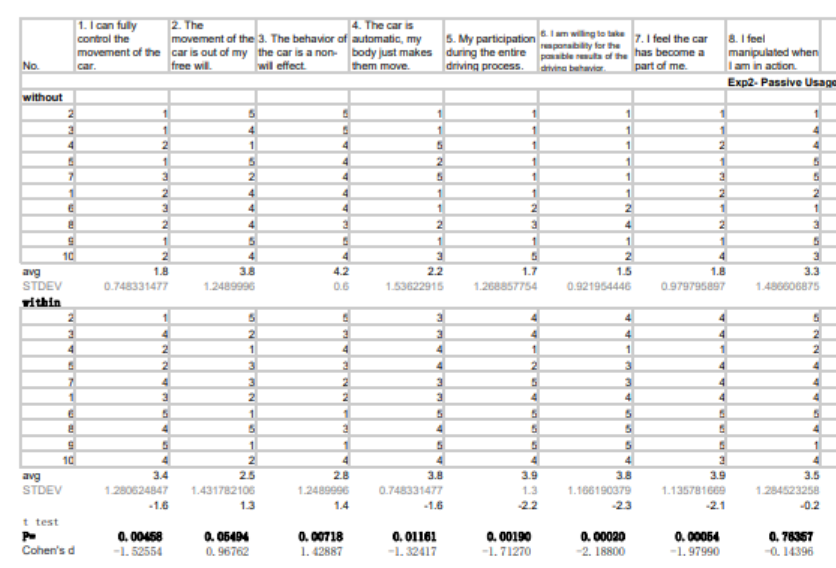
\includegraphics[width=0.8\textwidth]{A_thesis/figures/014-01.png}
\caption{Results on the sense of agency in passive use scenarios}
\end{figure}

In passive/inactive usage scenarios, the use of MotionPerformer greatly enhances users' sense of agency.

Q6: In passive driving situations, users refuse to take any responsibility for the consequences of the system's actions because they don't participate in any driving behaviors. However, after using MotionPerformer, by receiving the motion information of the vehicle, users' trust in the system is strengthened even though they are not involved in the driving process. This means they are more likely to trust the autonomous judgement of automation devices.

Q7: Despite emphasizing that users are in a simulated driving environment before the experiment, they still find it hard to feel that they and the vehicle have become a unity or that they have become the embodiment of the vehicle in the virtual environment. However, MotionPerformer can break the physical self-efficacy. It enhances the conveyance of motion information from automation devices to users, incorporating the automated devices into the users' framework of self. This generates a feeling that the vehicle has become a part of the user's body.

Q5: Before using the device, users do not have a significant sense of involvement, as the ideal situation often doesn't require users to make any actions during smart driving. However, using MotionPerformer greatly enhances users' sense of involvement in the movement process.

Q1: After using the device, users' perception of device control is enhanced. Even in passive usage scenarios, it still gives users a feeling of active control.

Among the negatively impacting parameters, the most significant ones are Q3 and Q4.

Q3: The behavior of the vehicle, which is not controlled by the user, is widely acknowledged in passive usage situations. However, after using MotionPerformer, users' judgement of autonomous actions begins to waver, leading them to question whether their intentions influence vehicle behavior during the driving process.

Q4: This reflects a similar problem. When it is mentioned that the system is automated and that user drives the automated motion behavior, users have a negative attitude in passive usage situations. However, after using MotionPerformer, users begin to acknowledge that even automation devices' movement behaviors can be influenced by the user themselves.

\subsubsection{Active Usage Scenarios}
\begin{figure}[h]
\centering
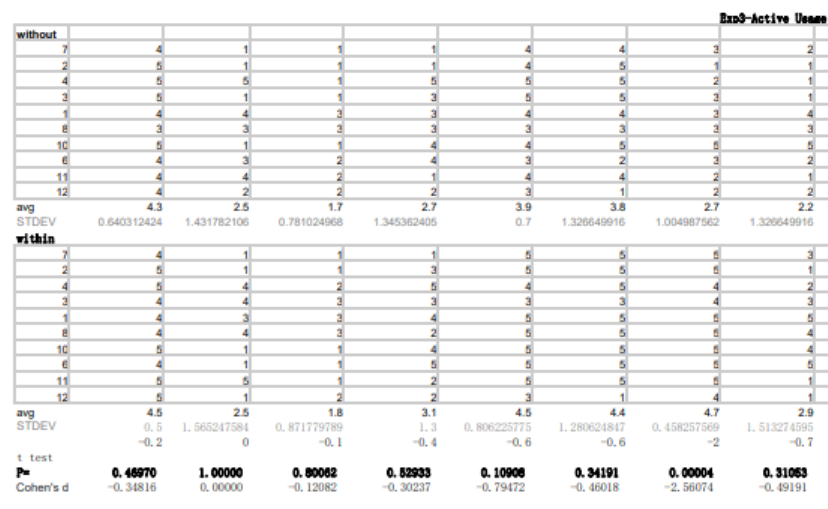
\includegraphics[width=0.8\textwidth]{A_thesis/figures/014-02.png}
\caption{Results on the sense of agency in active use scenarios}
\end{figure}

In active usage scenarios, since users are already independently controlling the vehicle's operation, the overall improvement in the sense of agency is very limited. The largest improvement is in Q7, where users acknowledge that by using MotionPerformer, the vehicle becomes a part of their own body. We believe that this not only enhances the sense of agency in driving but also changes and improves users' identity recognition. It allows users to reconsider the whole system's impact on them from their own cognitive perspective, rather than just from the perspective of an operator or driver.

\subsection{User Experience}

\begin{figure}[h]
\centering
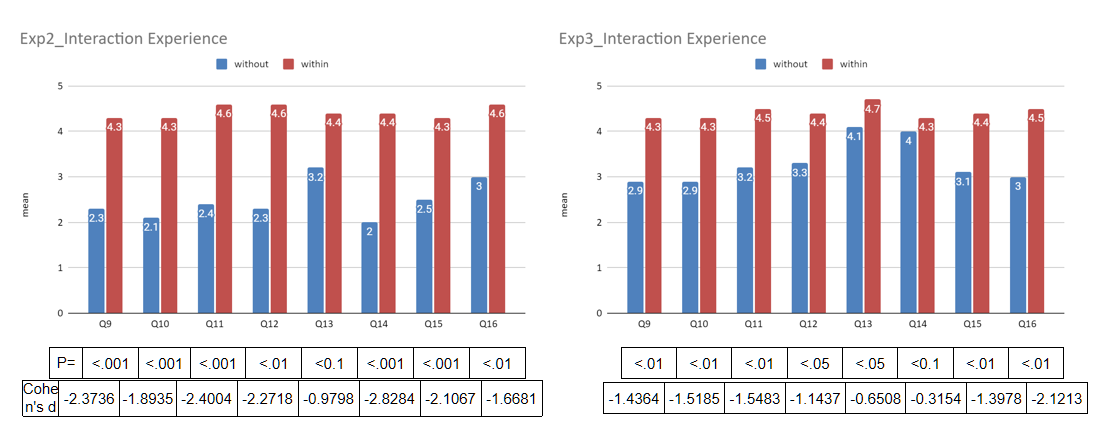
\includegraphics[width=0.9\textwidth]{A_thesis/figures/041.png}
\caption{Data visualization on user experience}
\end{figure}

\begin{figure}[h]
\centering
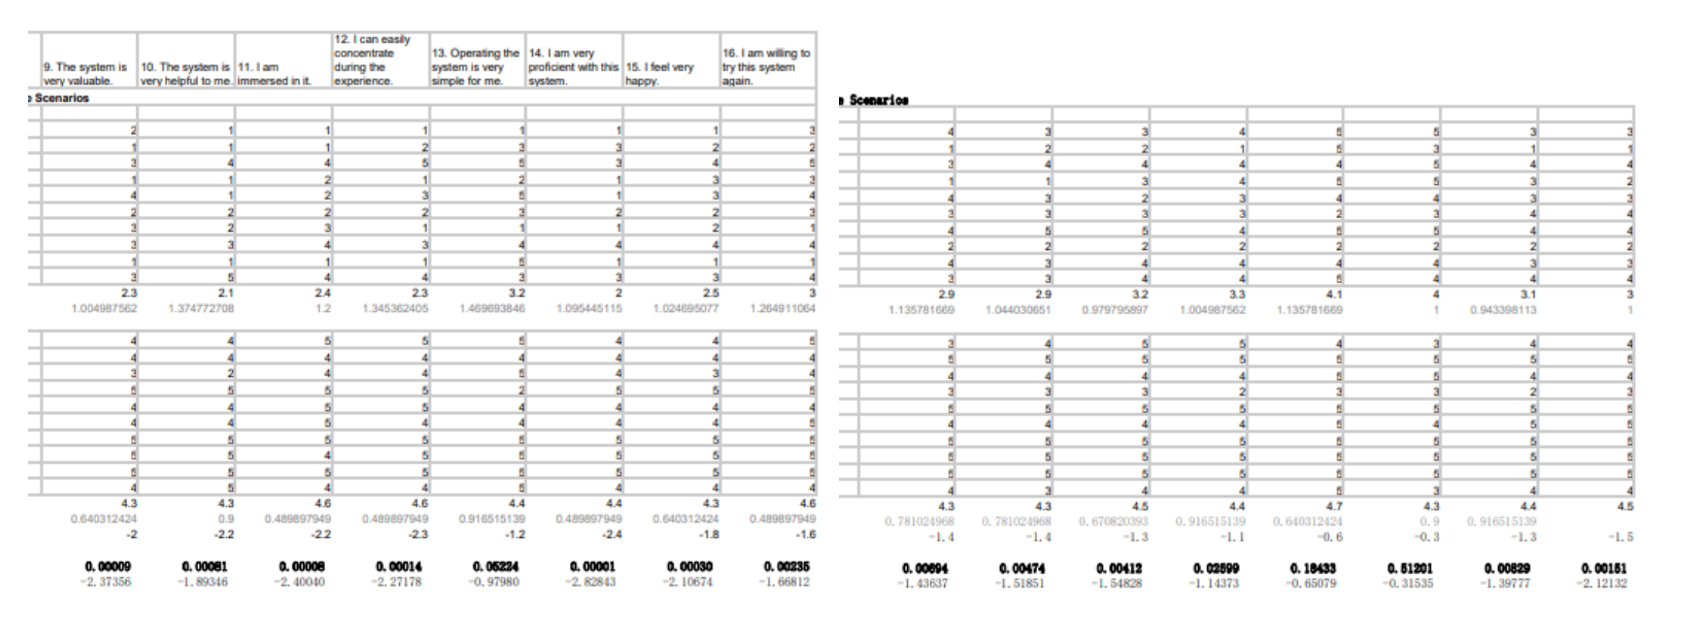
\includegraphics[width=0.95\textwidth]{A_thesis/figures/015.png}
\caption{Results on user experience}
\end{figure}

The last eight questions of the questionnaire mainly test the user's feeling and experience when using the MotionPerformer. In our original hypothesis, we thought that the active scenario might be more popular in terms of user experience, providing a greater experience. However, the results show that after introducing the MotionPerformer haptic system, the enhancement of the passive scenarios is greater than that of the active scenarios.

Q9 and Q10 primarily reflect whether the use of the MotionPerformer system is meaningful to users, and positive feedback was received in both usage scenarios. As previously mentioned by the users in their feedback, introducing MotionPerformer into the automation system helps users gain more information about the device's movement. In interactions with the intelligent system, having more information increases trust in the system. Users can also obtain information through haptic feedback that they didn't get visually.

Q11 and Q12 mainly reflect whether the user's immersion has increased after using the MotionPerformer system. In the passive usage scenario, users' sense of immersion has greatly improved. Feedback also mentioned that after gaining more haptic feedback, users will have more information for judgment. Interactions with the automation device will make users more willing to invest more attention into the operation of the automation system.

Q13 reflects whether the device is easy to control. Although the impact isn't as significant as other areas when combining both scenarios, the system itself is already relatively simple in the case of not using the device, so the improvement is very limited. However, We have reason to believe that in a more complex automation device, MotionPerformer can effectively reduce the complexity of operation.

Q14 is similar but not identical to Q13. Q14 mainly reflects mastery, this aspect mainly reflects the user's grasp and understanding of the entire system in the overall experience. It's worth noting that there is a significant impact difference between passive scenarios and active scenarios in this aspect. In the passive scenario, the effect is extremely significant. Like the improvement of the sense of agency, after receiving the haptic information provided by MotionPerformer, users no longer view the automation device as an independent system. Instead, they start to incorporate the automation device into their self-awareness through sharing haptic information and motion information. Since the acceptance of the device indicates that users will be superior in physical mastery and conceptual understanding compared to situations where haptics are not shared. In contrast to the results o passive scenarios, there is almost no significant improvement in this aspect in active scenarios. We believe that when users can already control the movement of objects, they have started to think from the perspective of the automation system or the pilot. Therefore, when the users has conceptually accepted the device, the improvement brought by MotionPerformer is not very effective.

Q15 and Q16 reflect whether MotionPerformer brings emotional value and enjoyment. Although both scenarios have achieved effective improvement in this aspect, the emotional value obviously has more improvement in the passive usage scenario. This represents that although users are in the interaction with the intelligent system, they would still choose a solution that brings haptic information. As for enjoyment, it's obviously more affected in the active scenario. Whether it's in a simulated driving scenario or a gaming application scenario, MotionPerformer brings rich haptic information, effectively enhancing the user's sense of entertainment.


\chapter{Conclusion}
This research begins with a brief introduction and review of HCI, VR, Haptic, etc., in Chapter 1, gradually narrowing down the field to finally determine the research direction of the motion state of self-moving objects. In Chapter 2, we draw inspiration and analysis from precedents in various classified fields, fully leverage the advantages of haptics compared to other sensory content, and compare our research plan with external design plans to determine the design idea and application scenarios of the final design plan. In Chapter 3, after trying and comparing different types of haptic device prototypes, we finally decided on a haptic design plan mainly presented through a roller. The goal is to convey to users the research objectives of the motion state of self-moving objects through haptics. In Chapter 4, we verified through experiments the effectiveness of MotionPerformer in transmitting motion information to users, including three main contents: displacement, rotation, and speed. Furthermore, two experiments were conducted to explore and verify that MotionPerformer can strengthen the interaction between users and future AI-powered/intelligent automation systems, and enhance experiences, immersion, and the entertainment of the system in virtual space under entertainment or simulation scenarios by adding haptic feedback.

Overall, the research objectives of this study have been basically achieved, and all hypotheses have been established. MotionPerformer can indeed effectively deliver the motion information of self-moving objects to users, but theoretically, the design plan of this study can improve the accuracy of specific information transmission of the device more effectively by replacing more efficient and reliable components. Moreover, there are still places in the design that are worth optimizing, such as adjusting the placement of components, optimizing the handheld design to wearable design, the visual effects and interaction system in the virtual scene are not complete enough, and the VR usage environment that did not appear in the design. All of these are worth updating in subsequent versions. However, through a relatively simple experimental environment, we still proved that such a haptic design as MotionPerformer can enhance the interaction and connection between users and intelligent automation systems in the future, such as the driving scenario in this research. Users can indeed perceive the sense of agency of active driving in an inactive driving environment through MotionPerformer, which has a very positive role in considering how to interact with intelligent automation systems, such as drones and robots in the future. And most importantly, MotionPerformer has strong versatility. Its positive impact is not only manifested in automation interactions, it can be used in any virtual scene's user-avatar interaction process, and effectively enhance user immersion and interactivity. 

In summary, MotionPerformer can help users establish a force reference in virtual space or non-real operation environments, share motion information between the user and the interactive object, and we believe this will bring more experiences and possibilities to future human-computer interaction methods.

%\input{TP_1_Introduction}
%\input{TP_2-relatedworks-en}
%\input{implementation-jp.tex}
%\input{evaluation-jp.tex}
%\input{conclusion-jp.tex}
%
%
%%%%%%%%%%%%%%%%%%%%%%%%%%%%%%%%%%%%%%%%%%%%%%%%%%%%%%%%%%%%%%%%%%%%
%%%%%%%%%%%%%%%%%%%%%%%%%%%%%%%%%%%%%%%%%%%%%%%%%%%%%%%%%%%%%%%%%%%%
%
% Just chapter name at the end of main text
%
\def\chaptermark#1{\markboth{#1}{ }}%


\newpage

%%%%%%%%%%%%%%%%
% Bibliography %
%%%%%%%%%%%%%%%%

%
% Bibliography
% Using BibTeX (pbibtex) is suggested. You can also create the
% list of referances with \reference.
%

%
% Use to list all references given to bibtex.
% Don't modify if you need referenaces only cited in the text.
%
% \ifDRAFT
%    \nocite{*}
% \fi

\bibliography{thesis-en}

%%%%%%%%%%%%%%%%%%%%%%%%%
% Style of Bibliography %
%%%%%%%%%%%%%%%%%%%%%%%%%
%
\ifCHICAGO
   \bibliographystyle{econ_edit}
\else
   \bibliographystyle{unsrt-url}
\fi
%
%%%%%%%%%%%%%%%%%%%%%%%
%
% Appendix if any
%
\appendix
\def\chaptermark#1{\markboth{\thechapter.\ #1}{ }}%
%
% !TEX root = thesis-en.tex
\section{Core Code of the Unity Project File}
\begin{figure}[h]
\centering
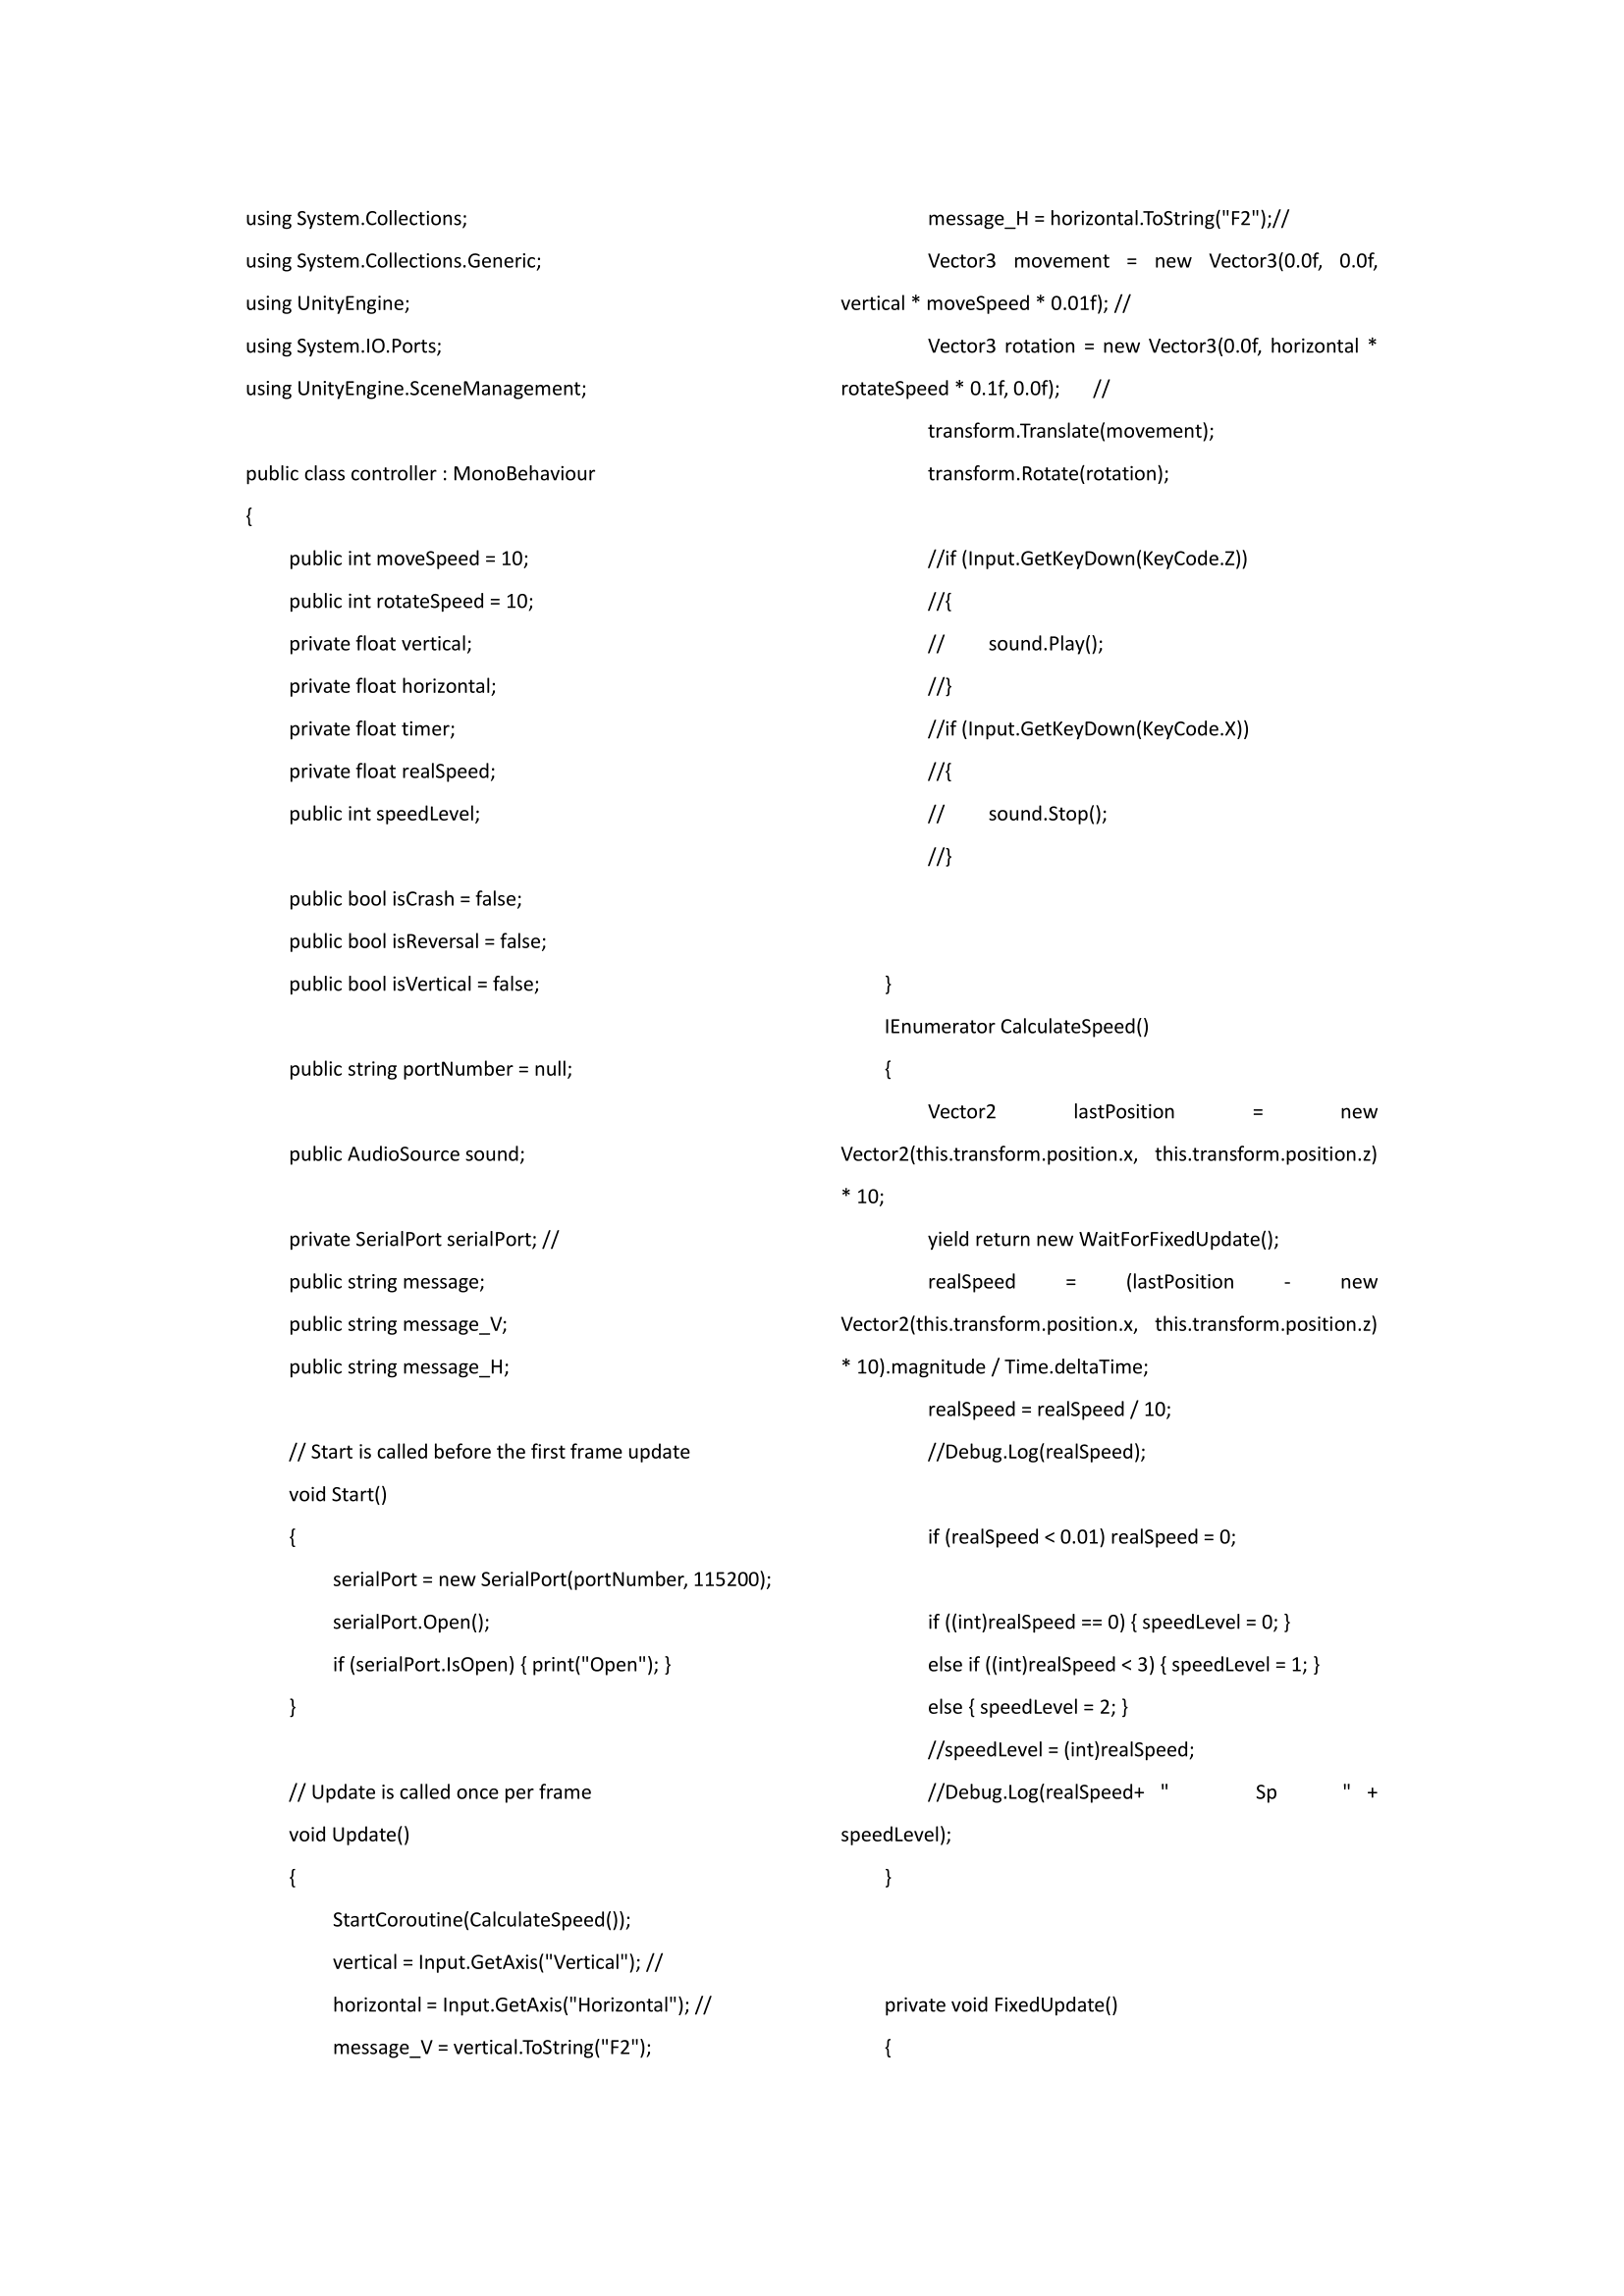
\includegraphics[width=1\textwidth,height=0.7\textheight]{A_thesis/appendix/code_unity-1.png}
\end{figure}
\newpage

\begin{figure}[h]
\centering
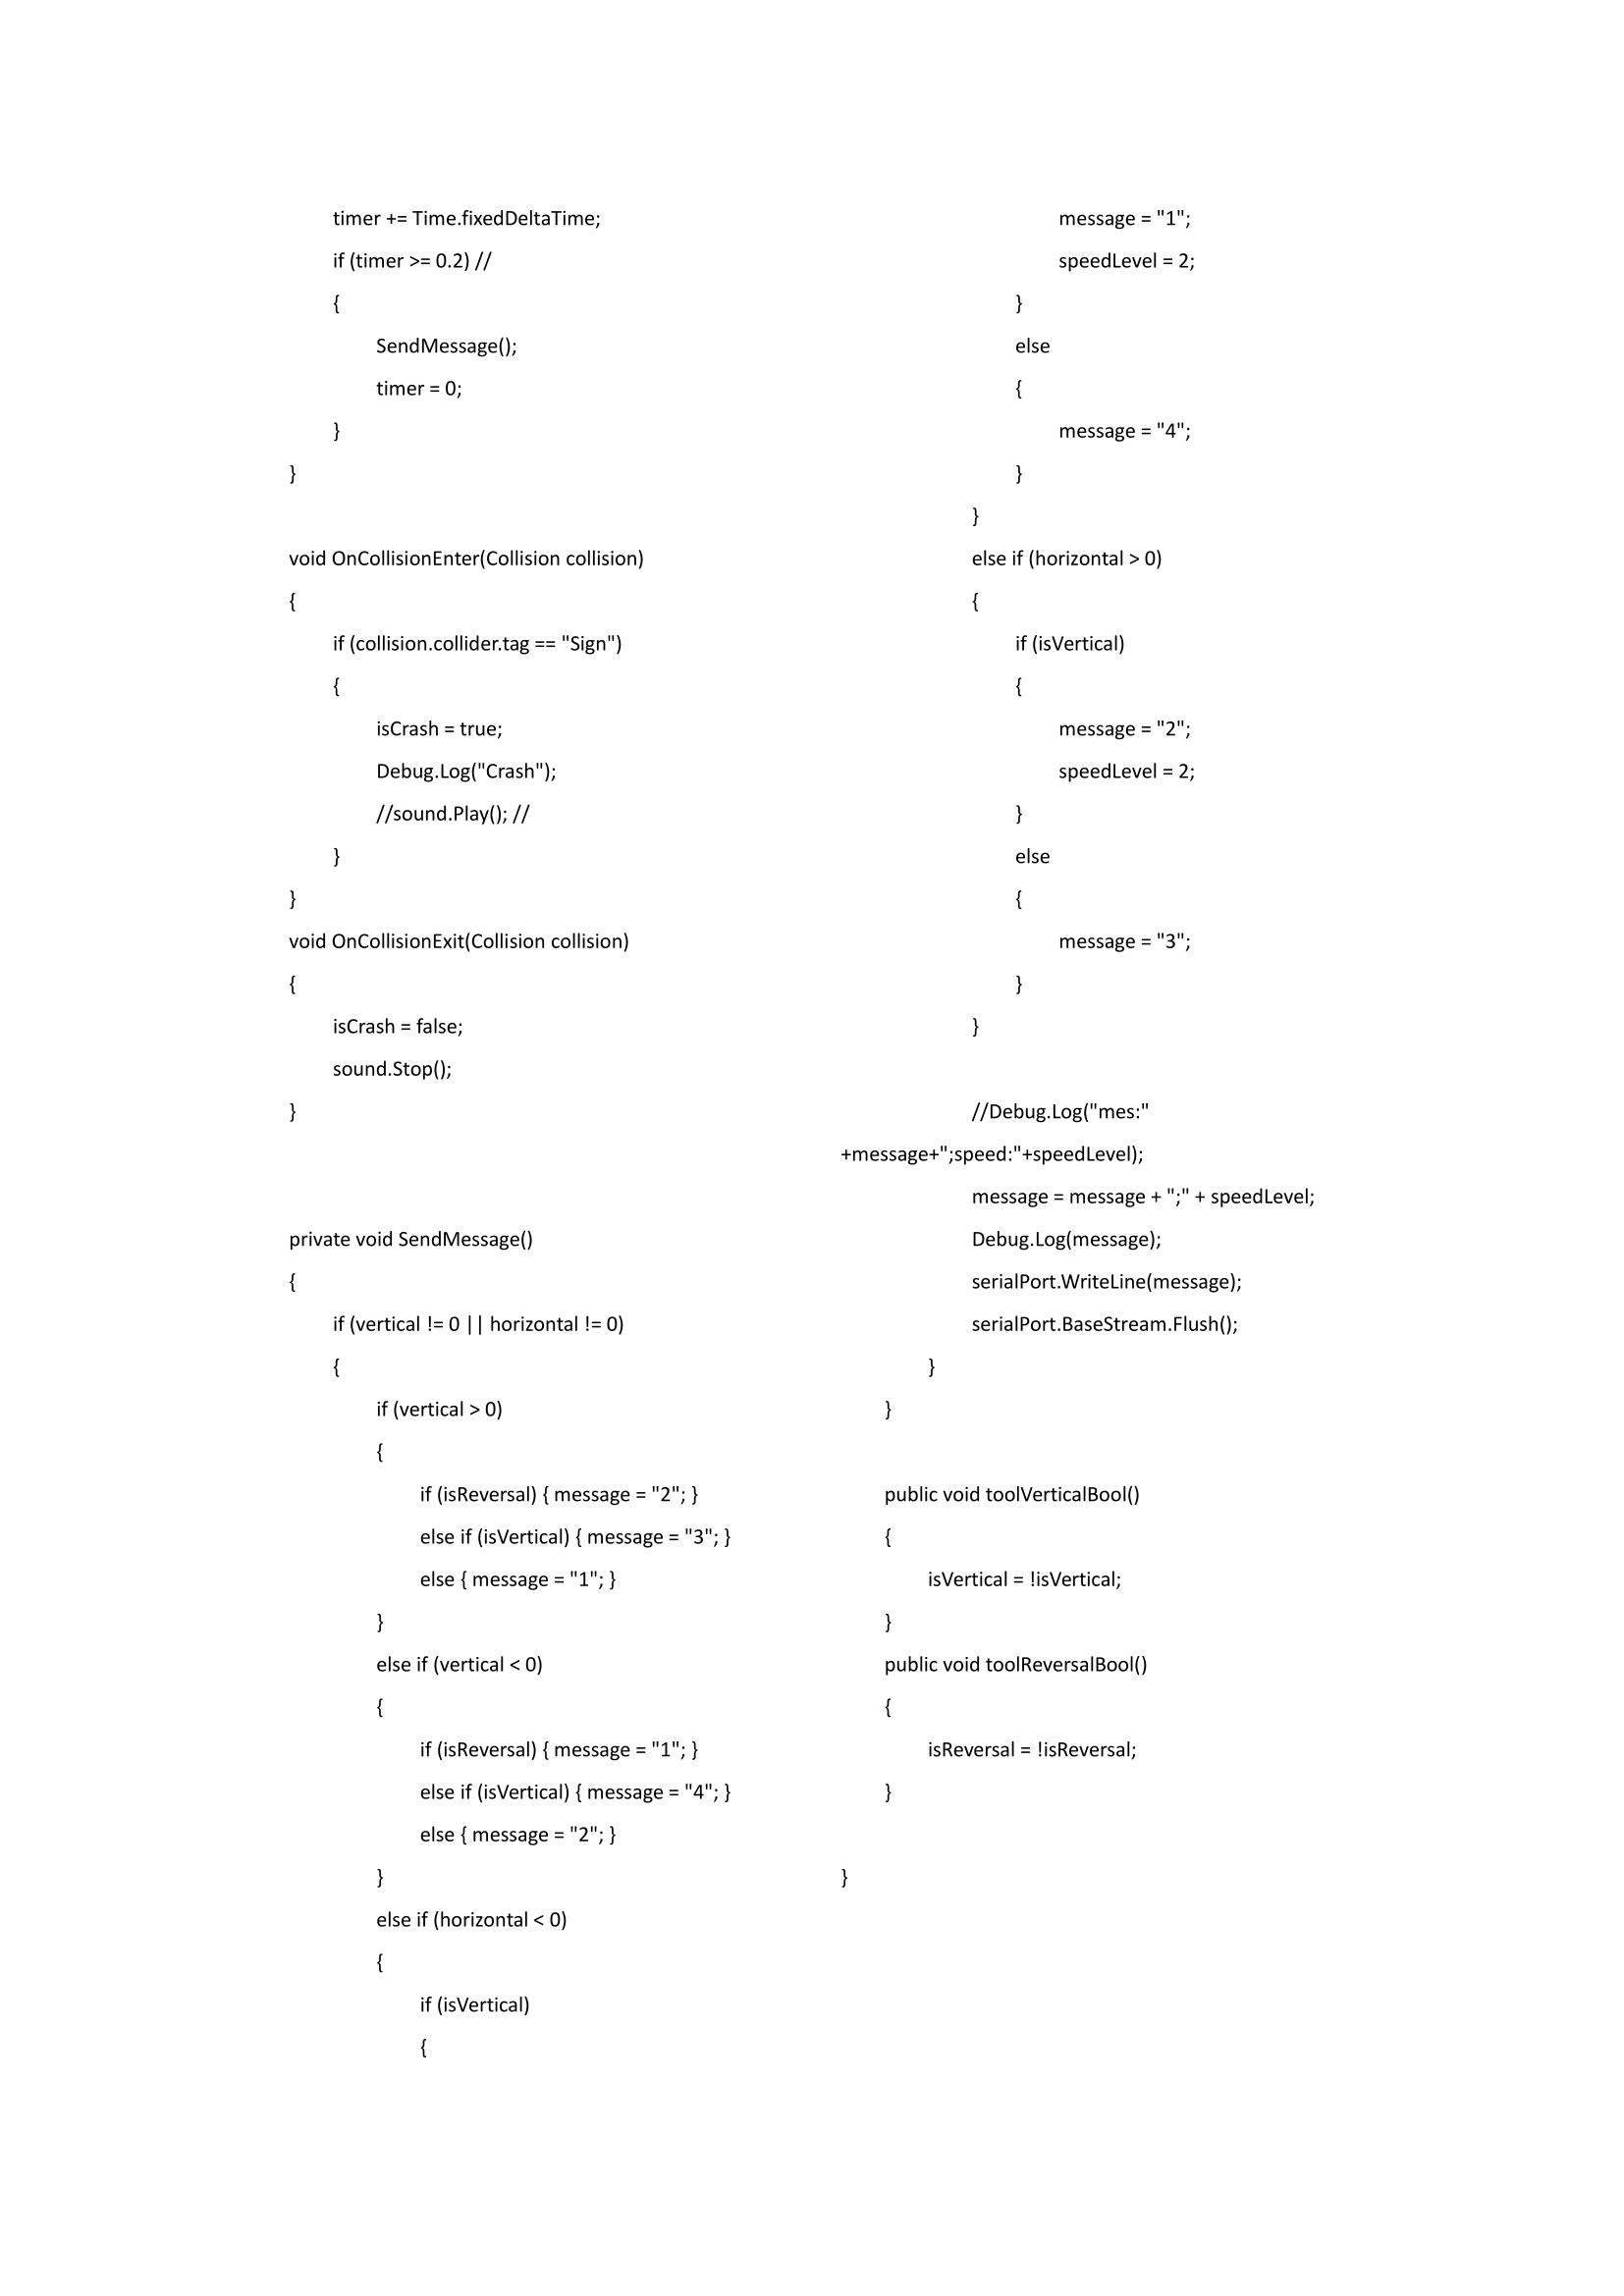
\includegraphics[width=1\textwidth,height=0.7\textheight]{A_thesis/appendix/code_unity-2.png}
\end{figure}
\newpage

\section{Core Code of the Arduino Project File}
\begin{figure}[h]
\centering
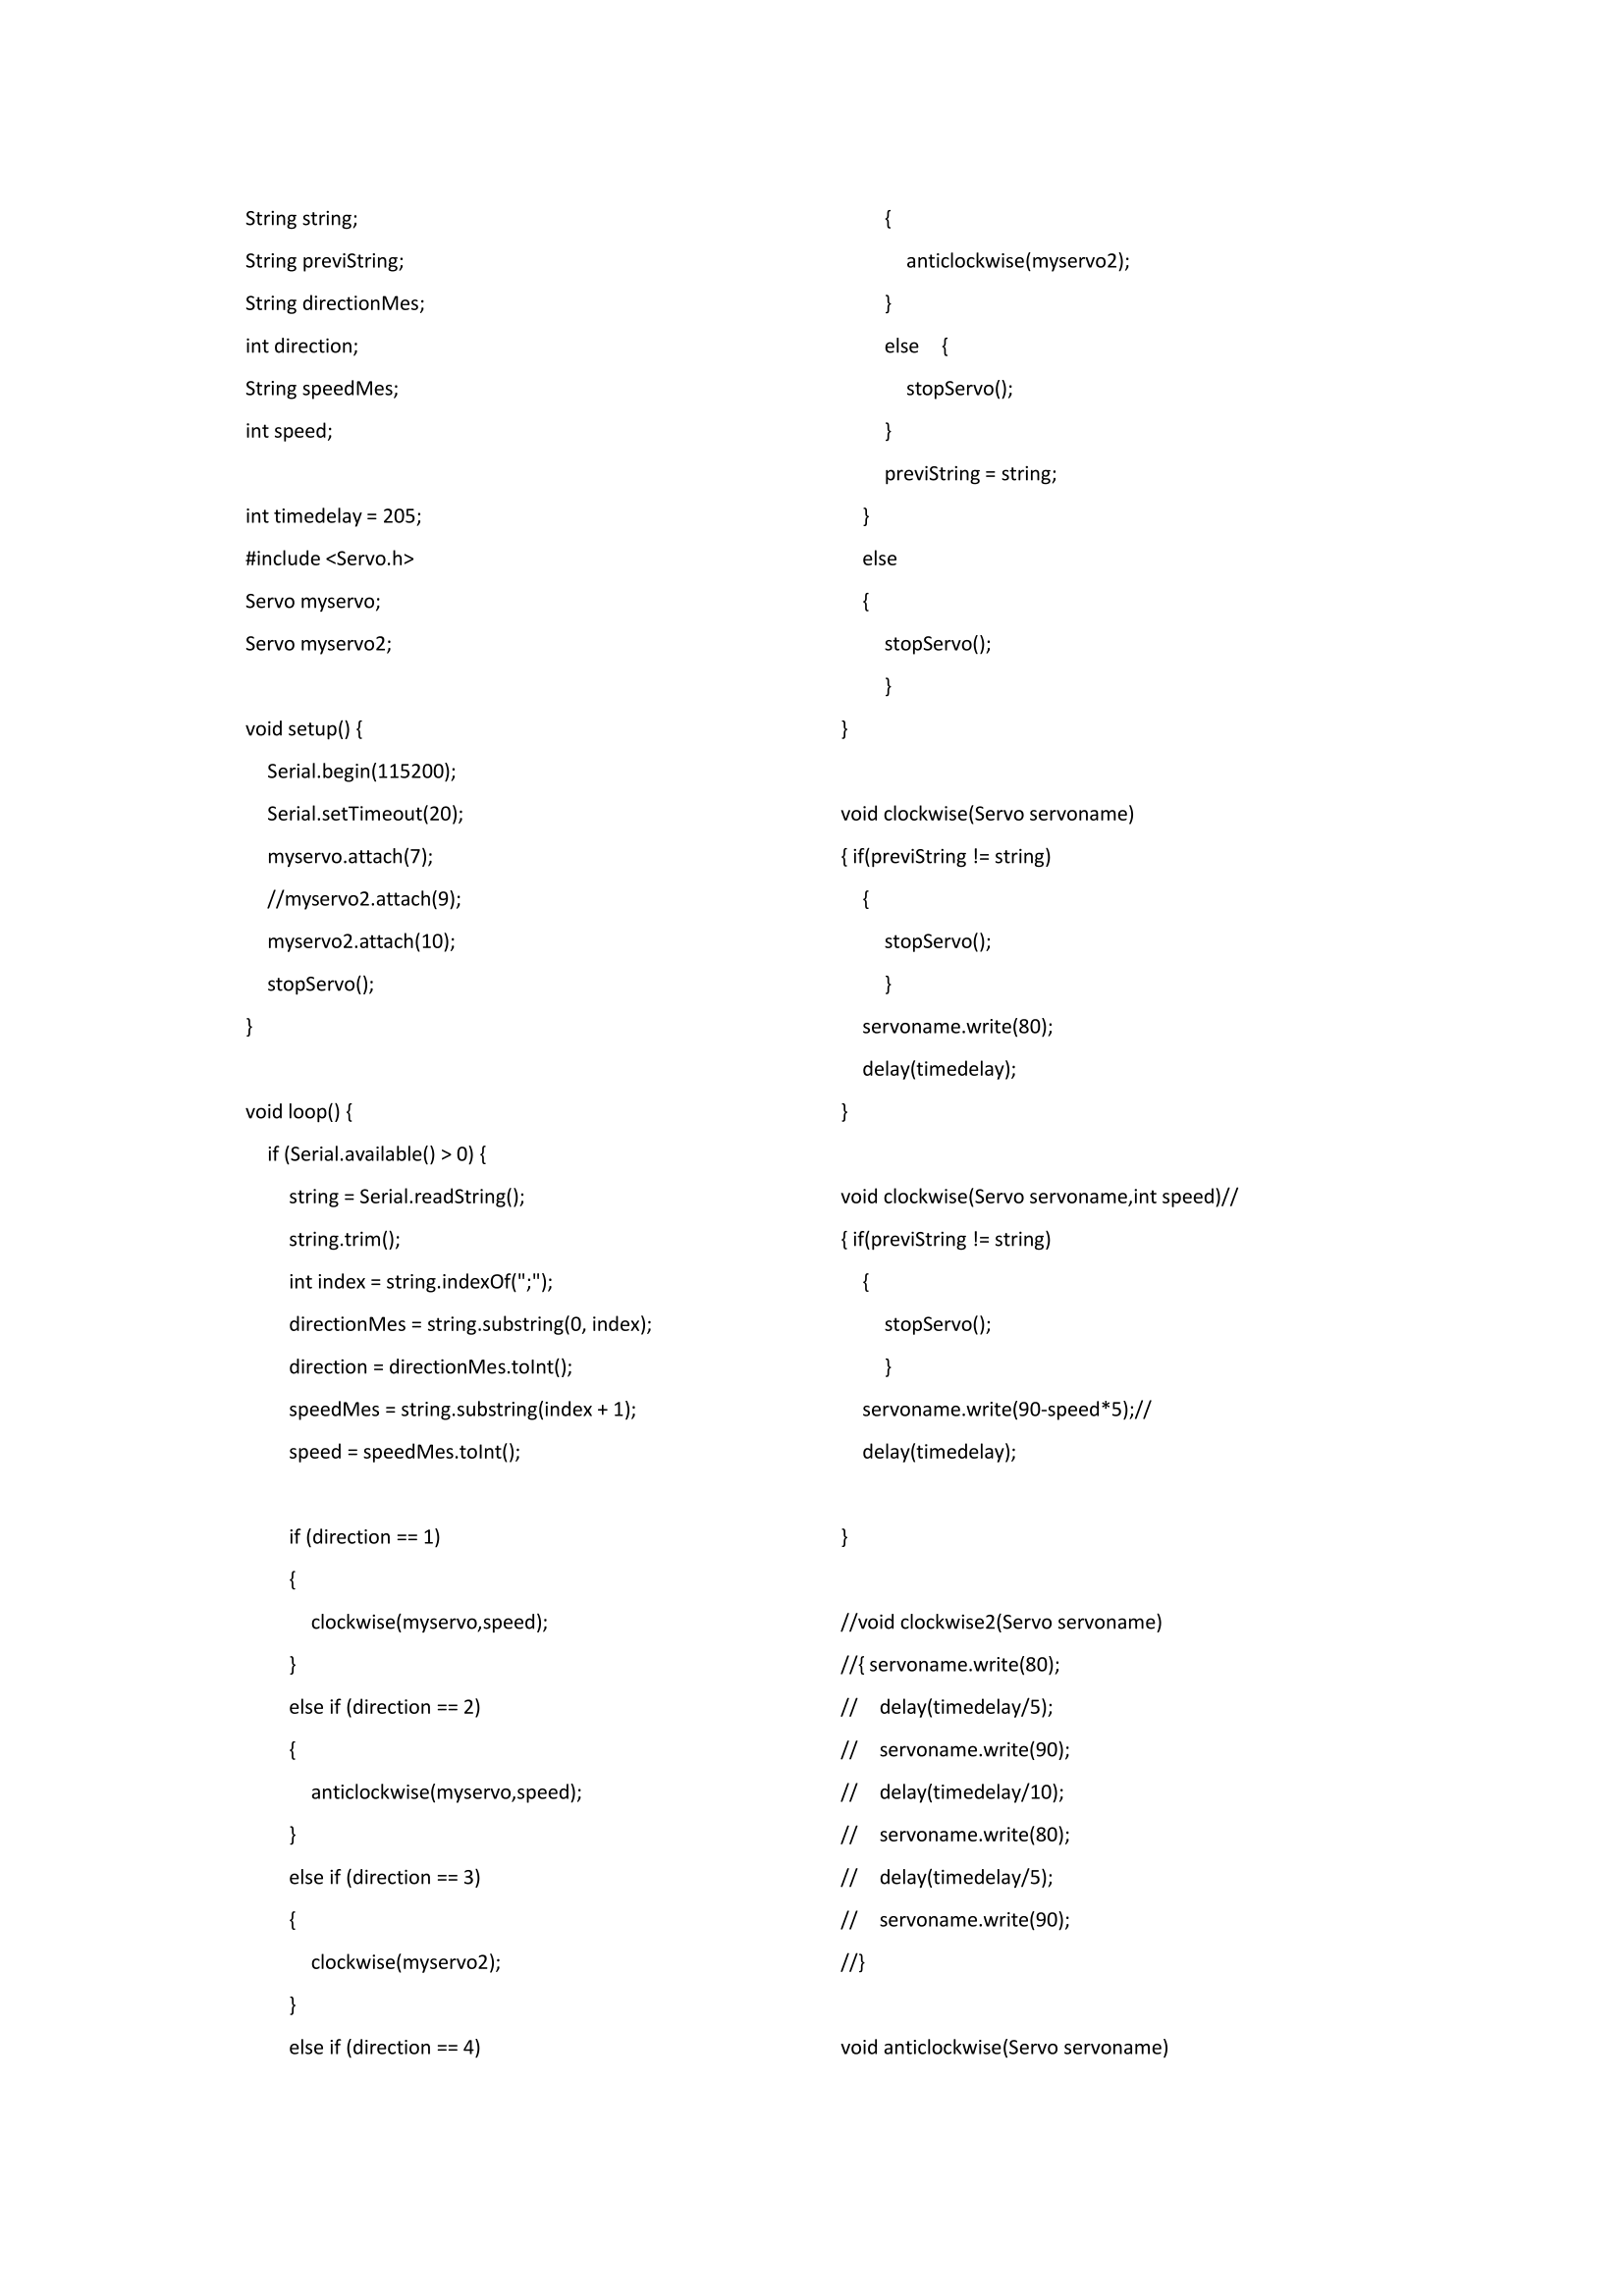
\includegraphics[width=1\textwidth,height=0.7\textheight]{A_thesis/appendix/code_arduino-1.png}
\end{figure}
\newpage

\begin{figure}[h]
\centering
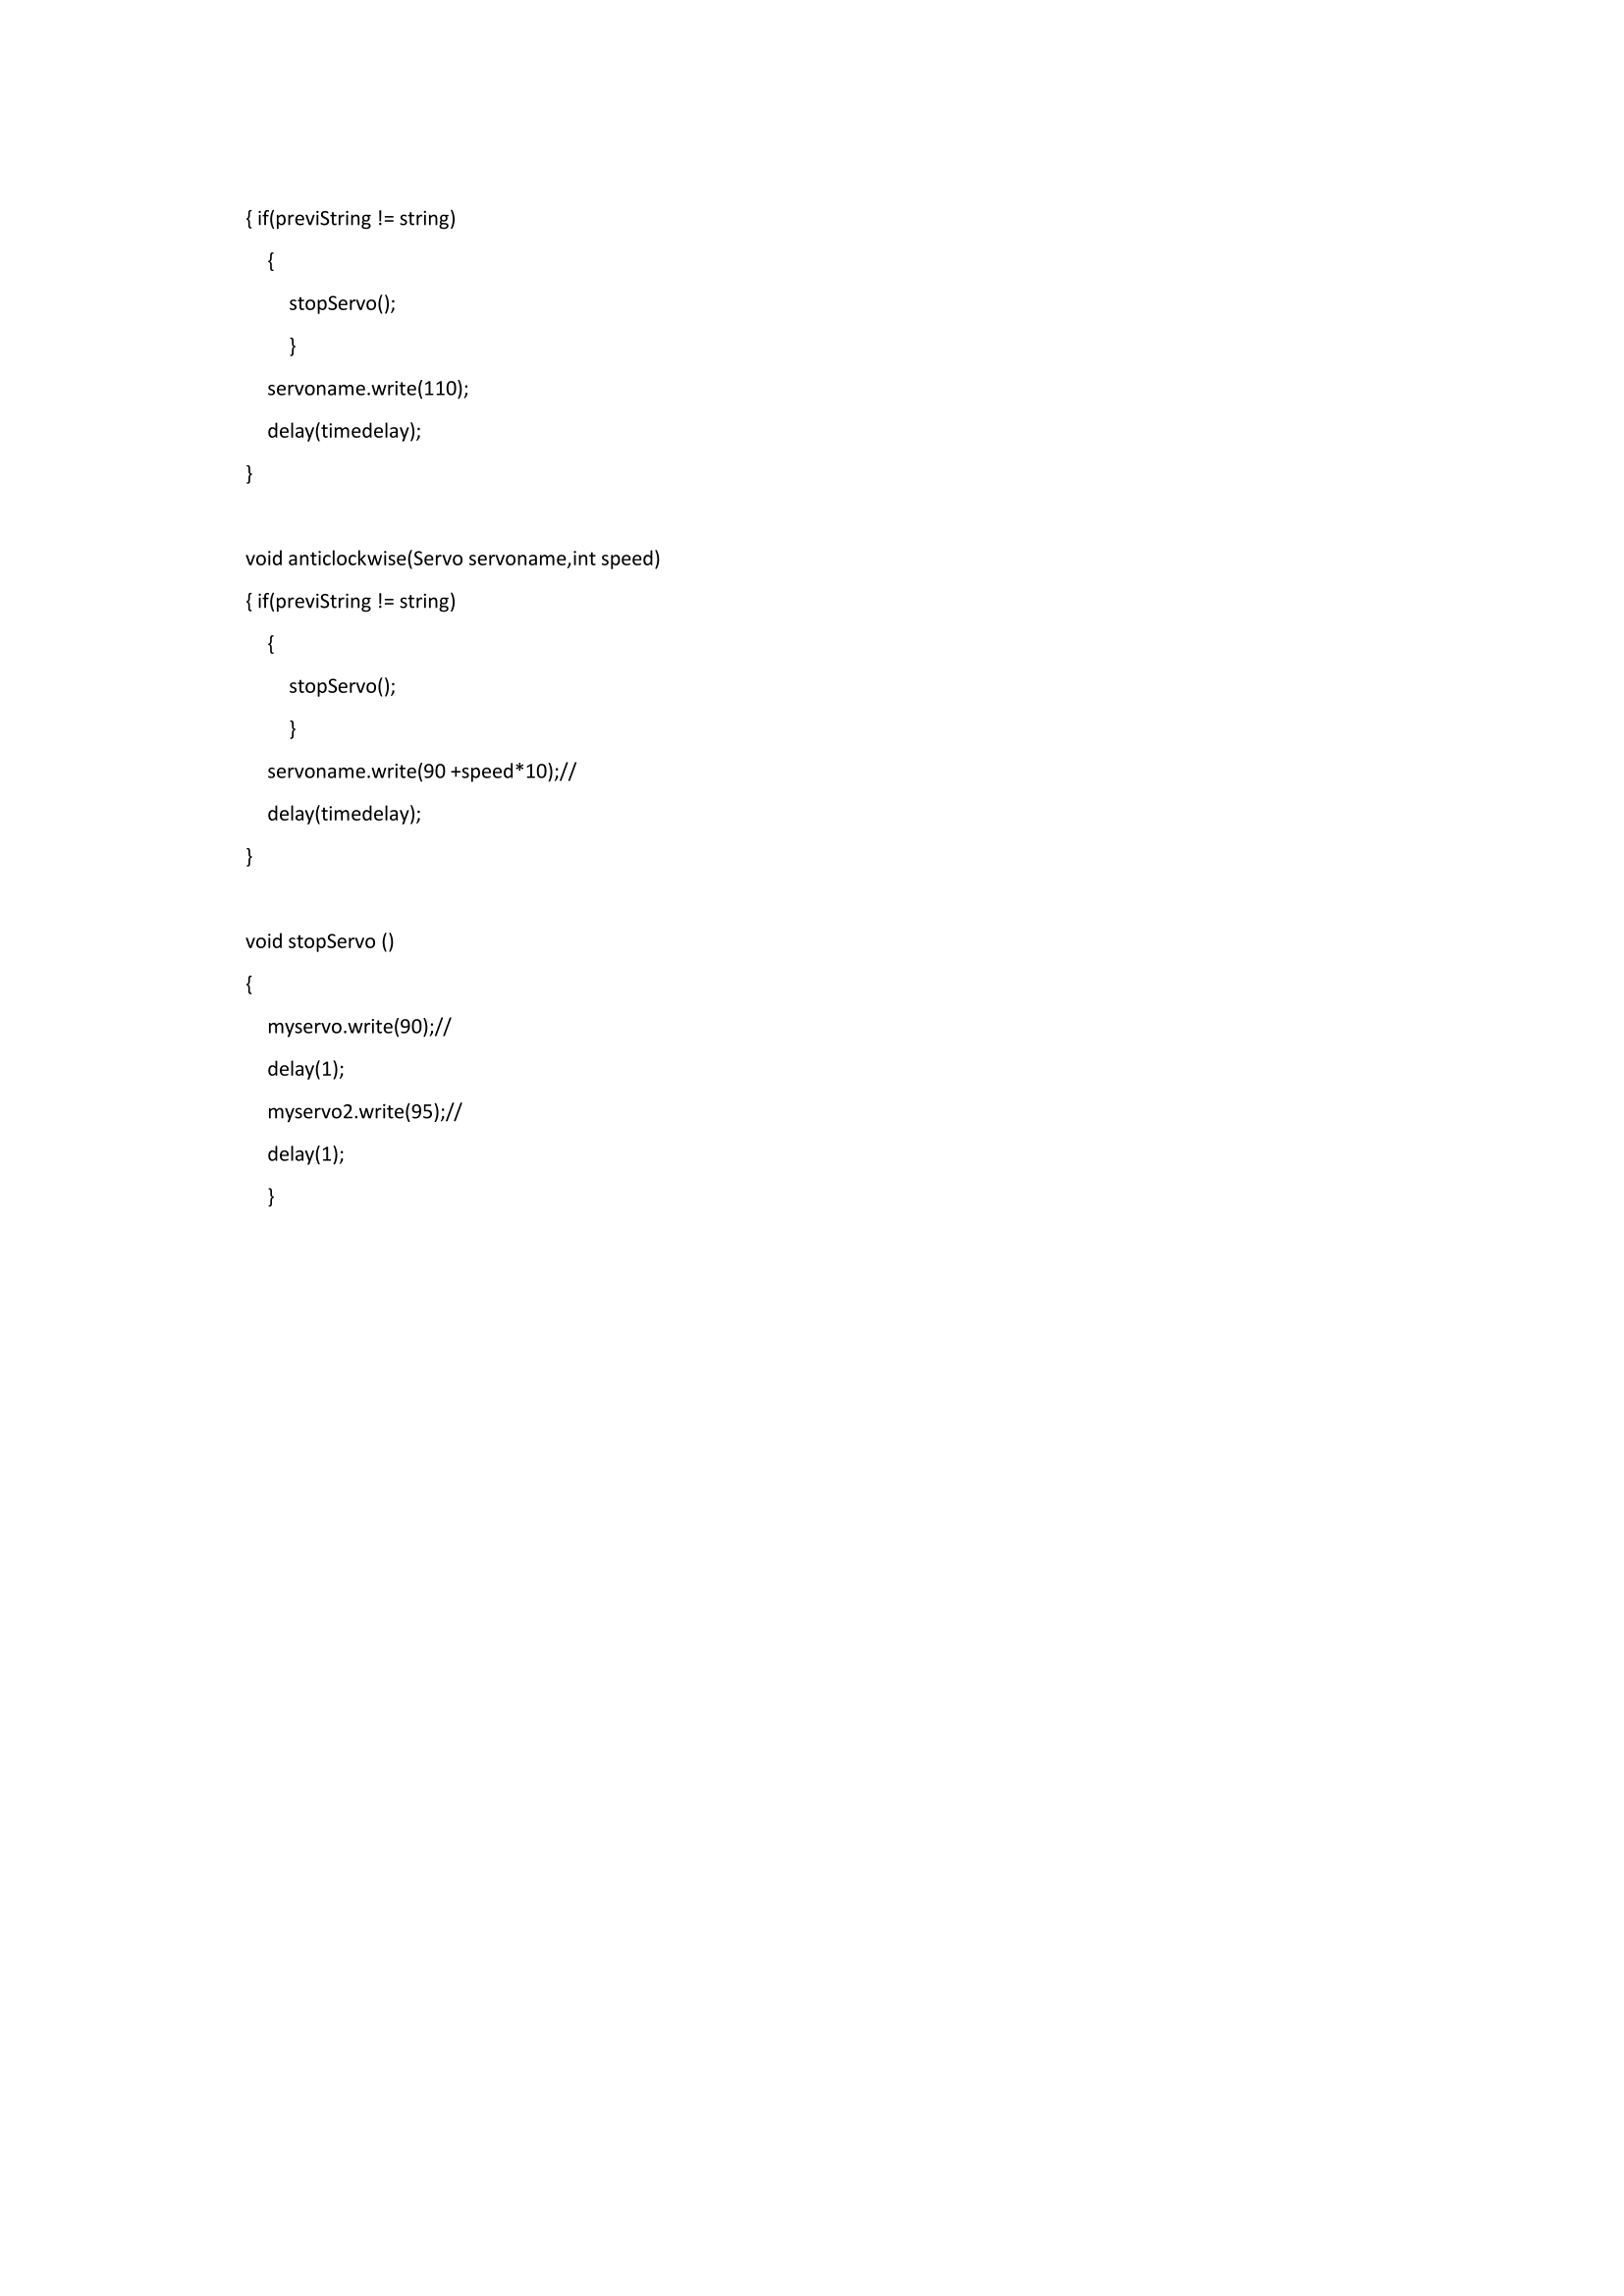
\includegraphics[width=1\textwidth,height=0.7\textheight]{A_thesis/appendix/code_arduino-2.png}
\end{figure}
\newpage

\section{Questionnaire of the Experiment1}
\begin{figure}[h]
\centering
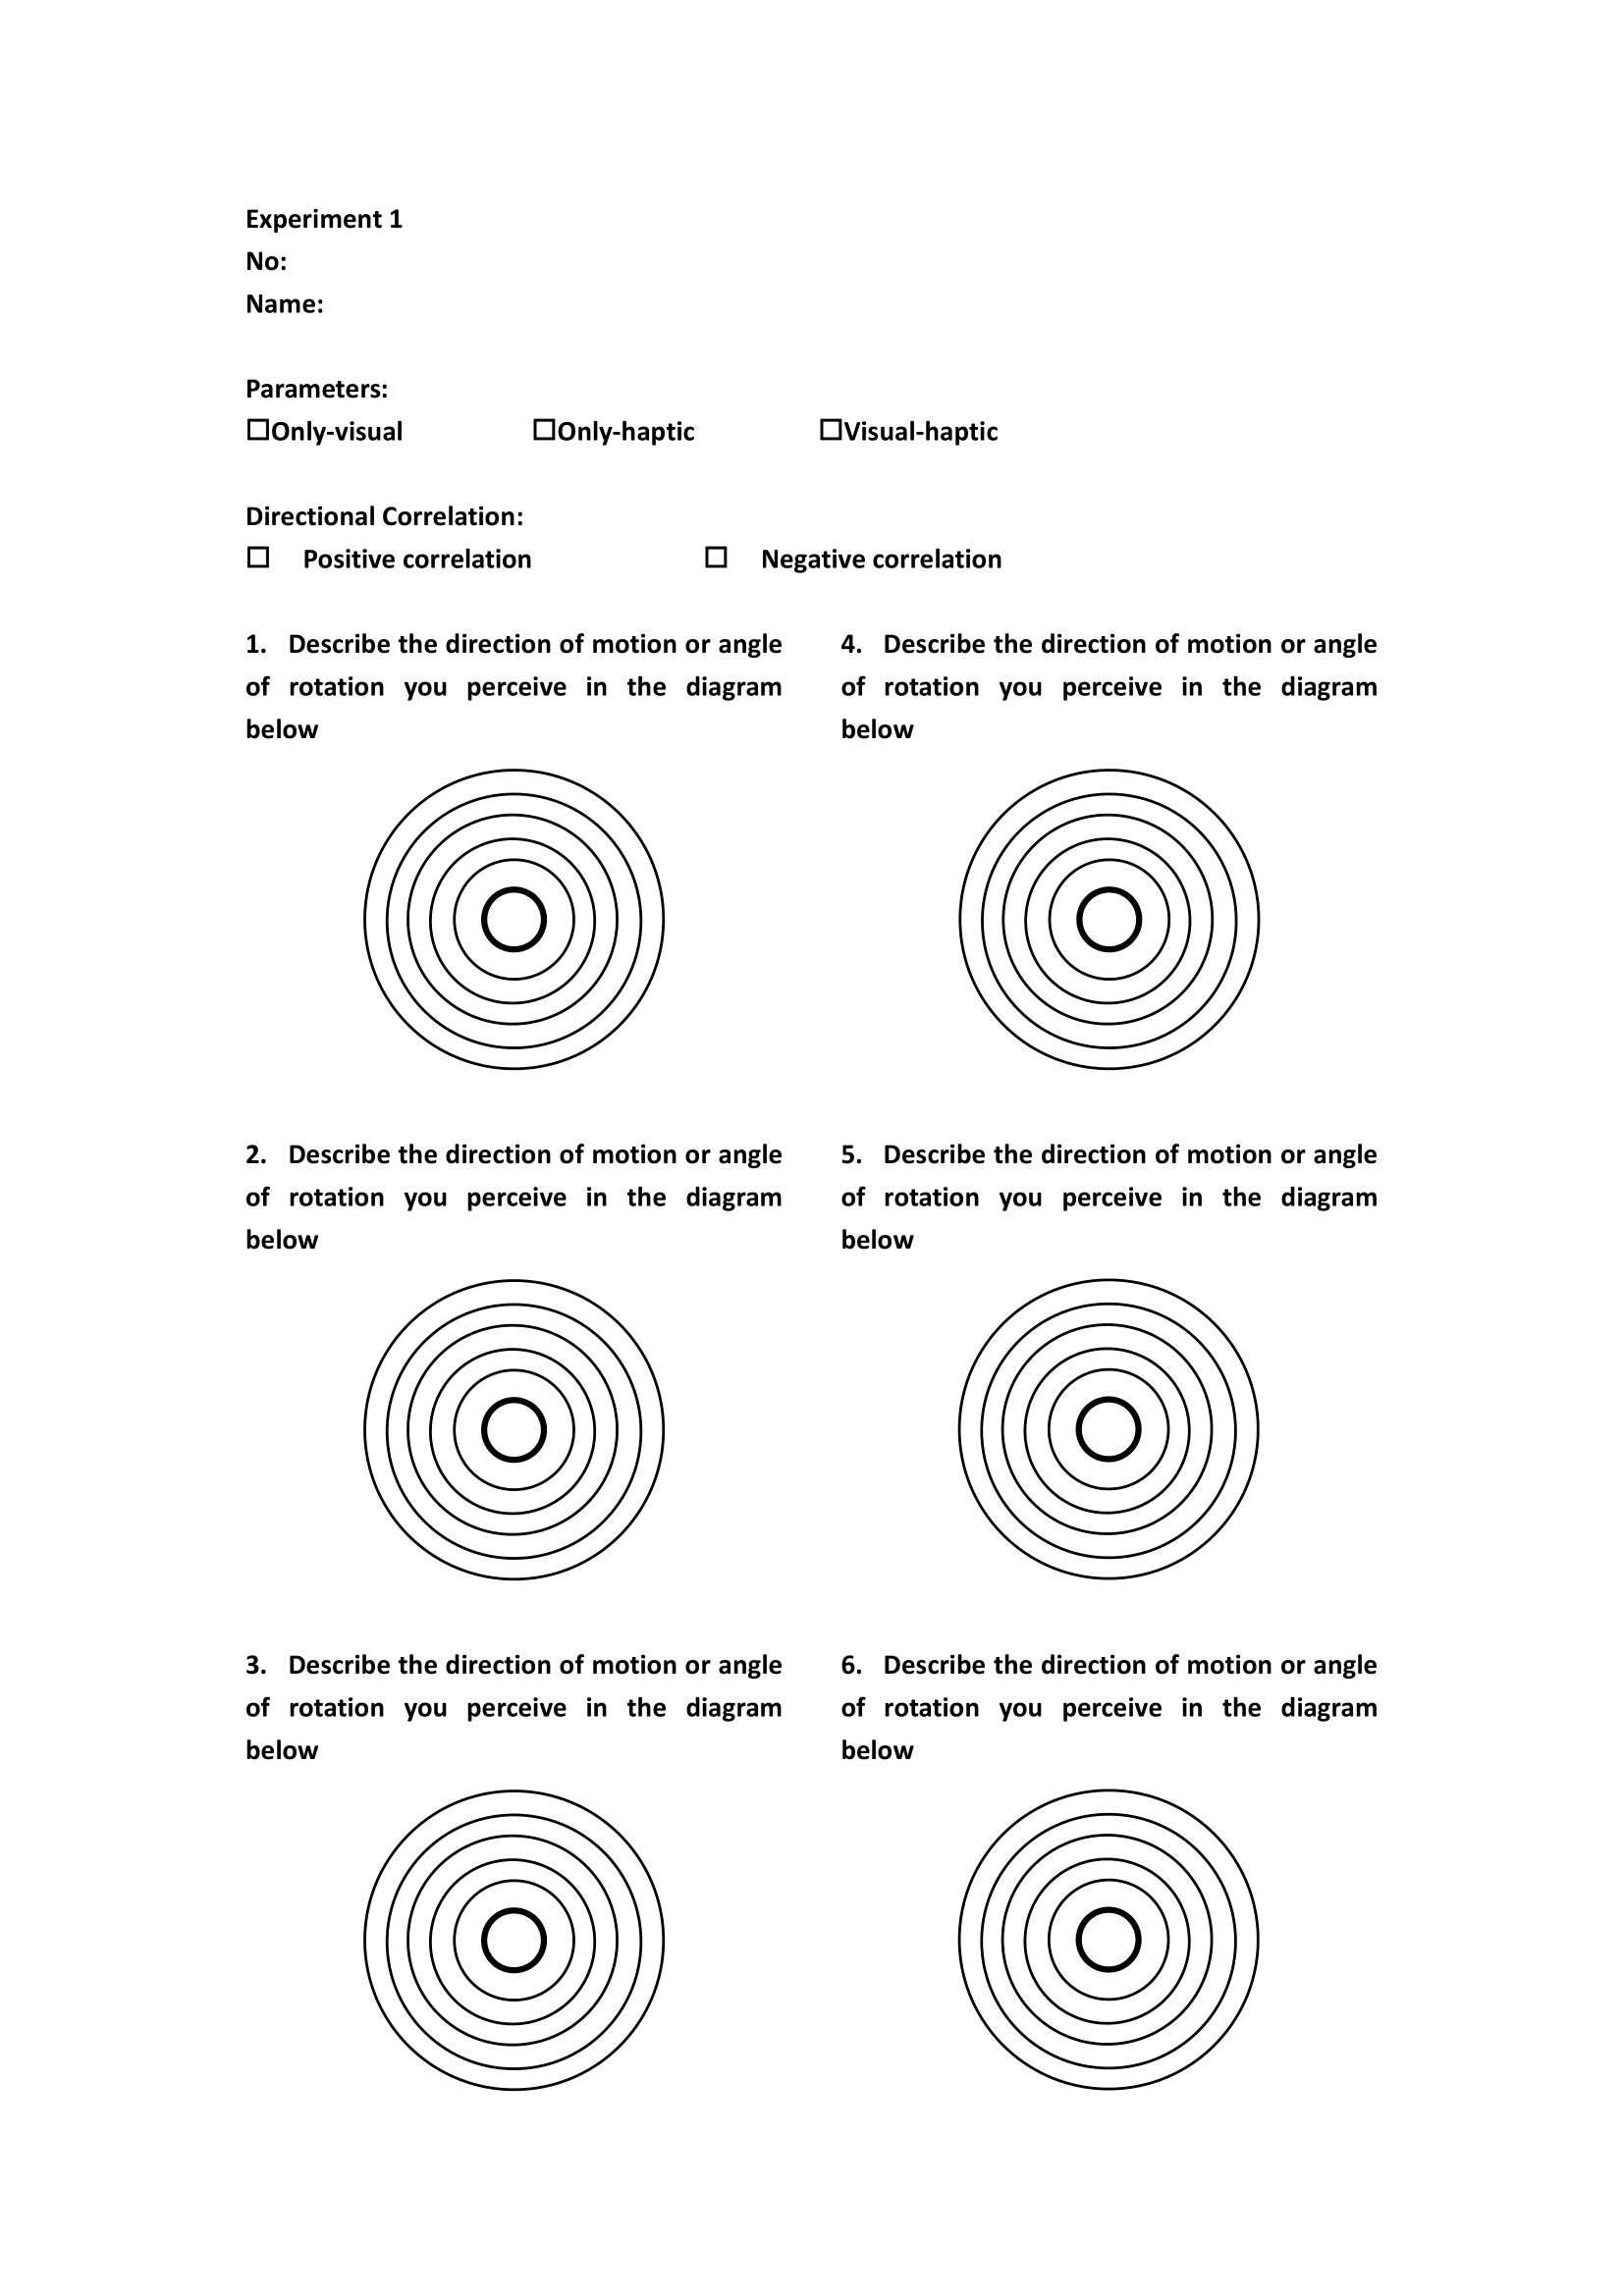
\includegraphics[width=1\textwidth,height=0.7\textheight]{A_thesis/appendix/Experiment1_questionnaire-1.png}
\end{figure}
\newpage

\begin{figure}[h]
\centering
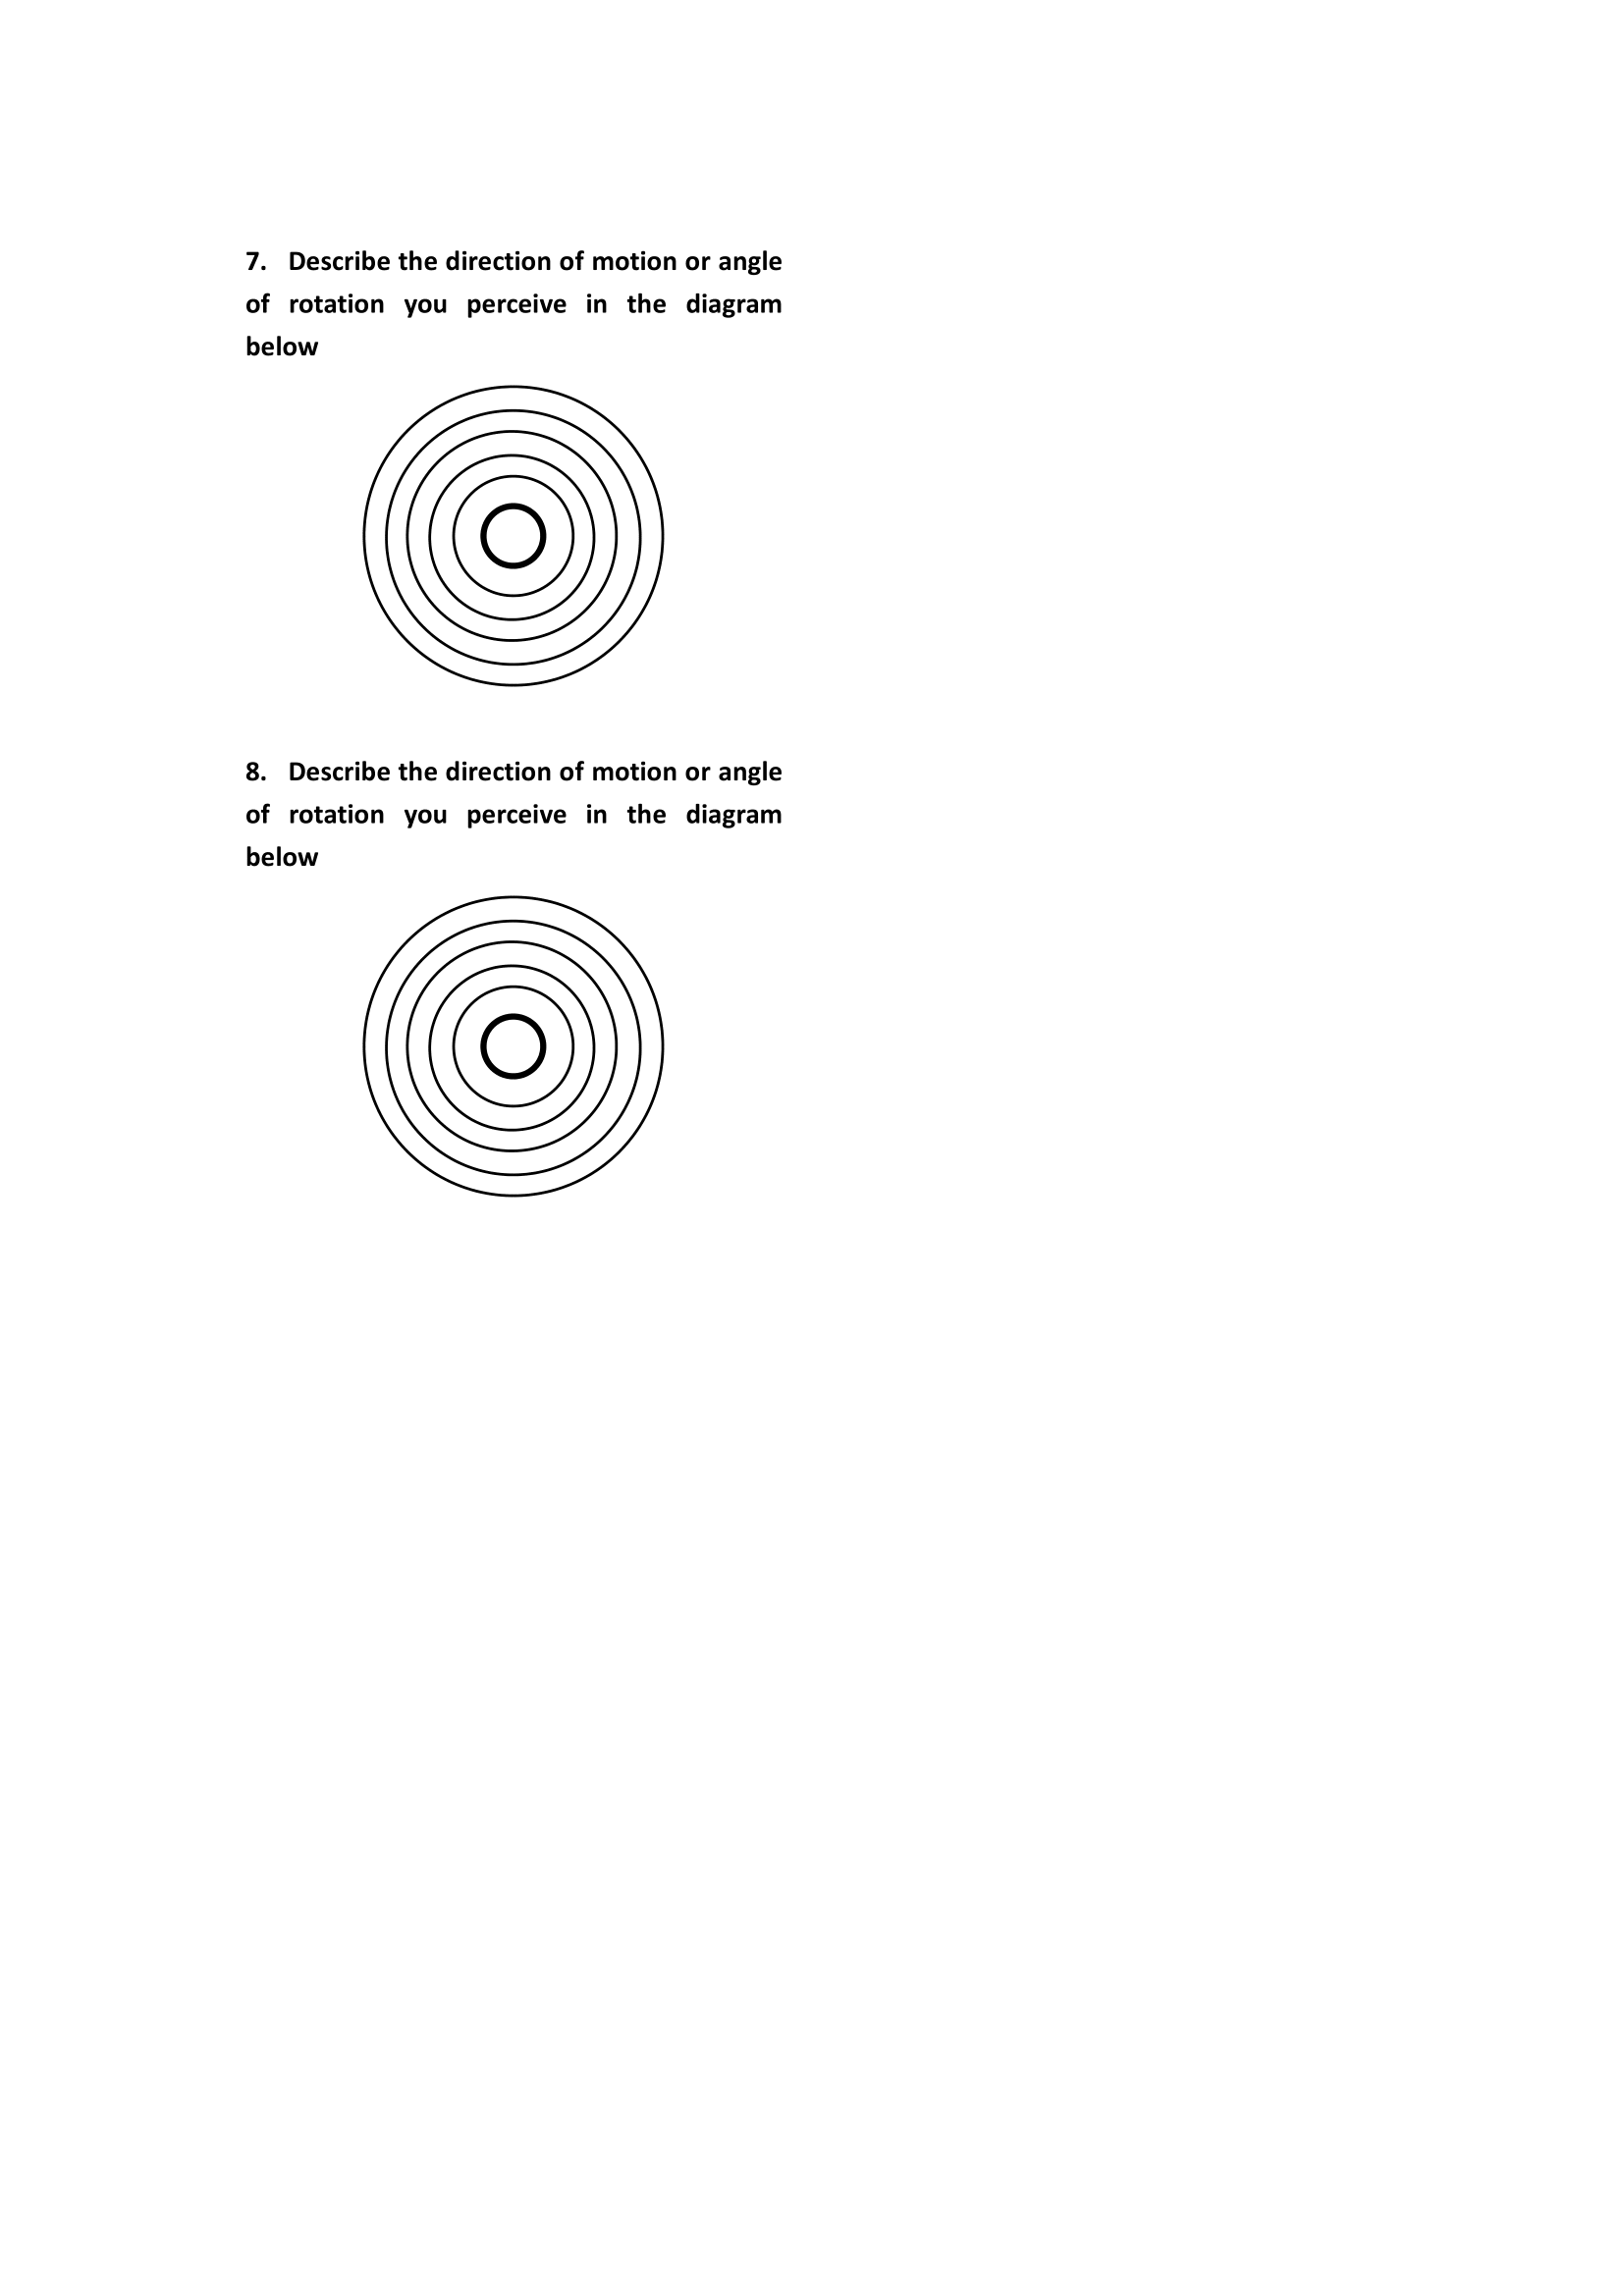
\includegraphics[width=1\textwidth,height=0.7\textheight]{A_thesis/appendix/Experiment1_questionnaire-2.png}
\end{figure}
\newpage

\begin{figure}[h]
\centering
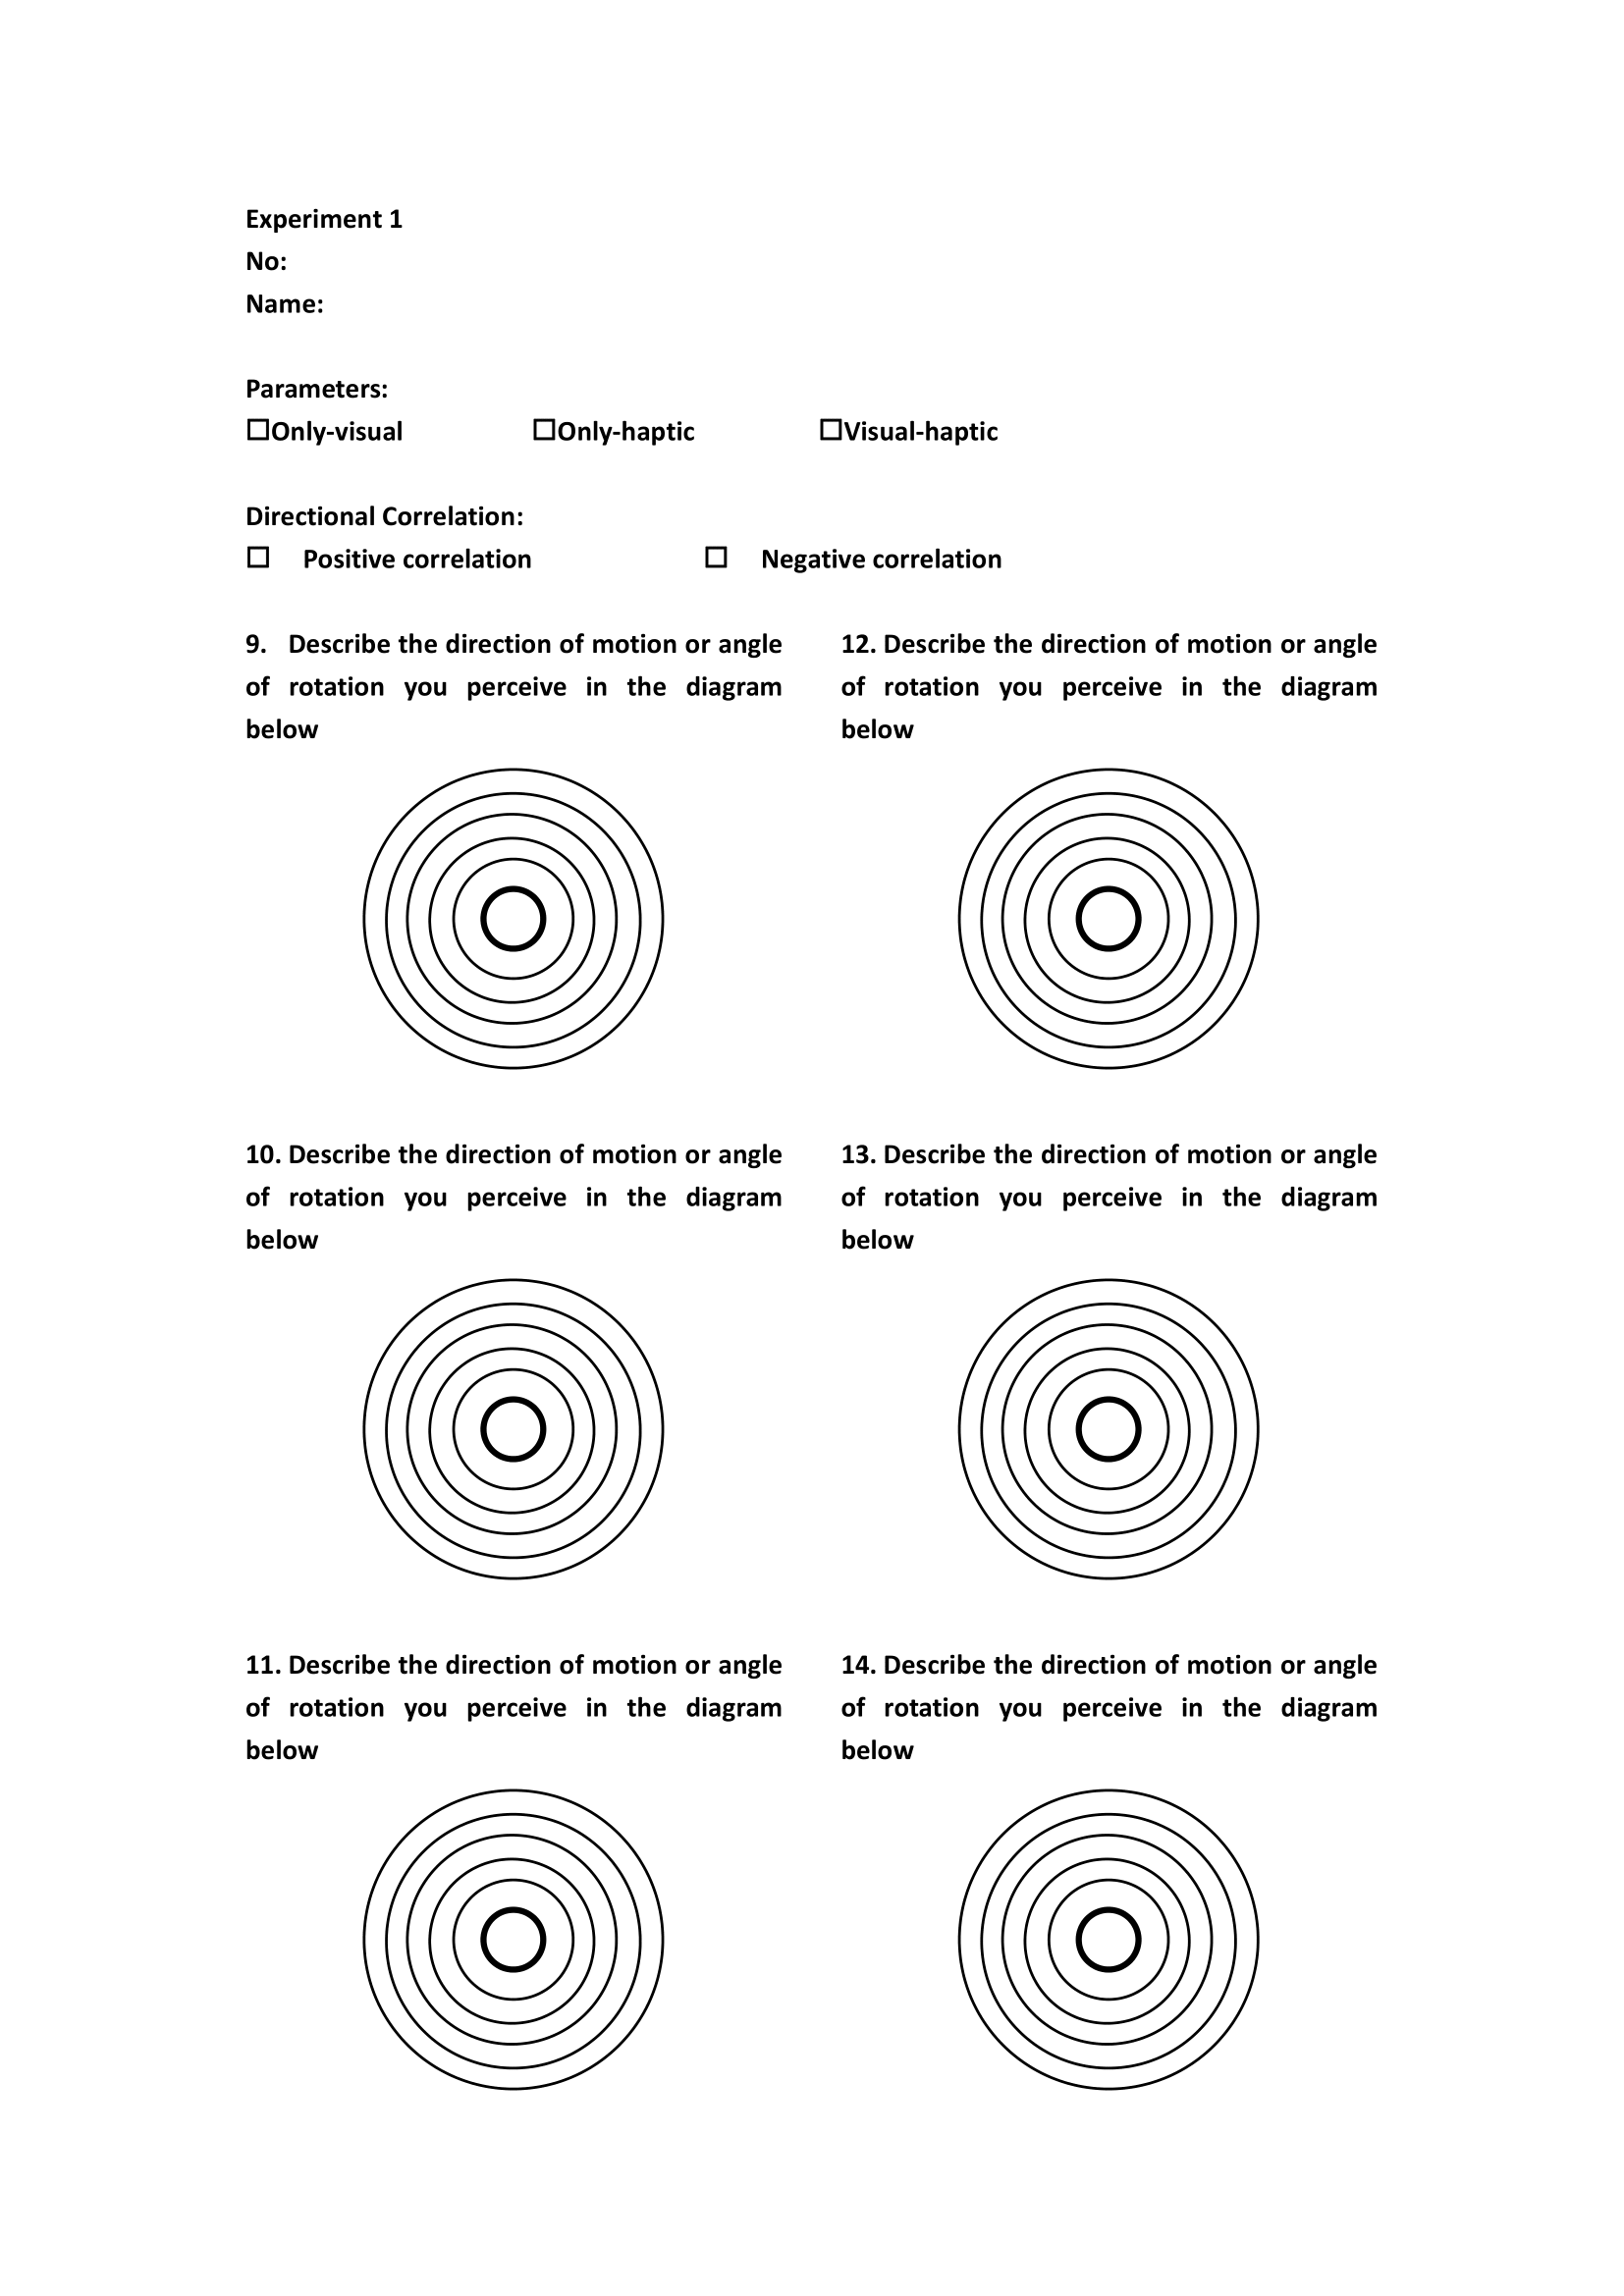
\includegraphics[width=1\textwidth,height=0.7\textheight]{A_thesis/appendix/Experiment1_questionnaire-3.png}
\end{figure}
\newpage

\begin{figure}[h]
\centering
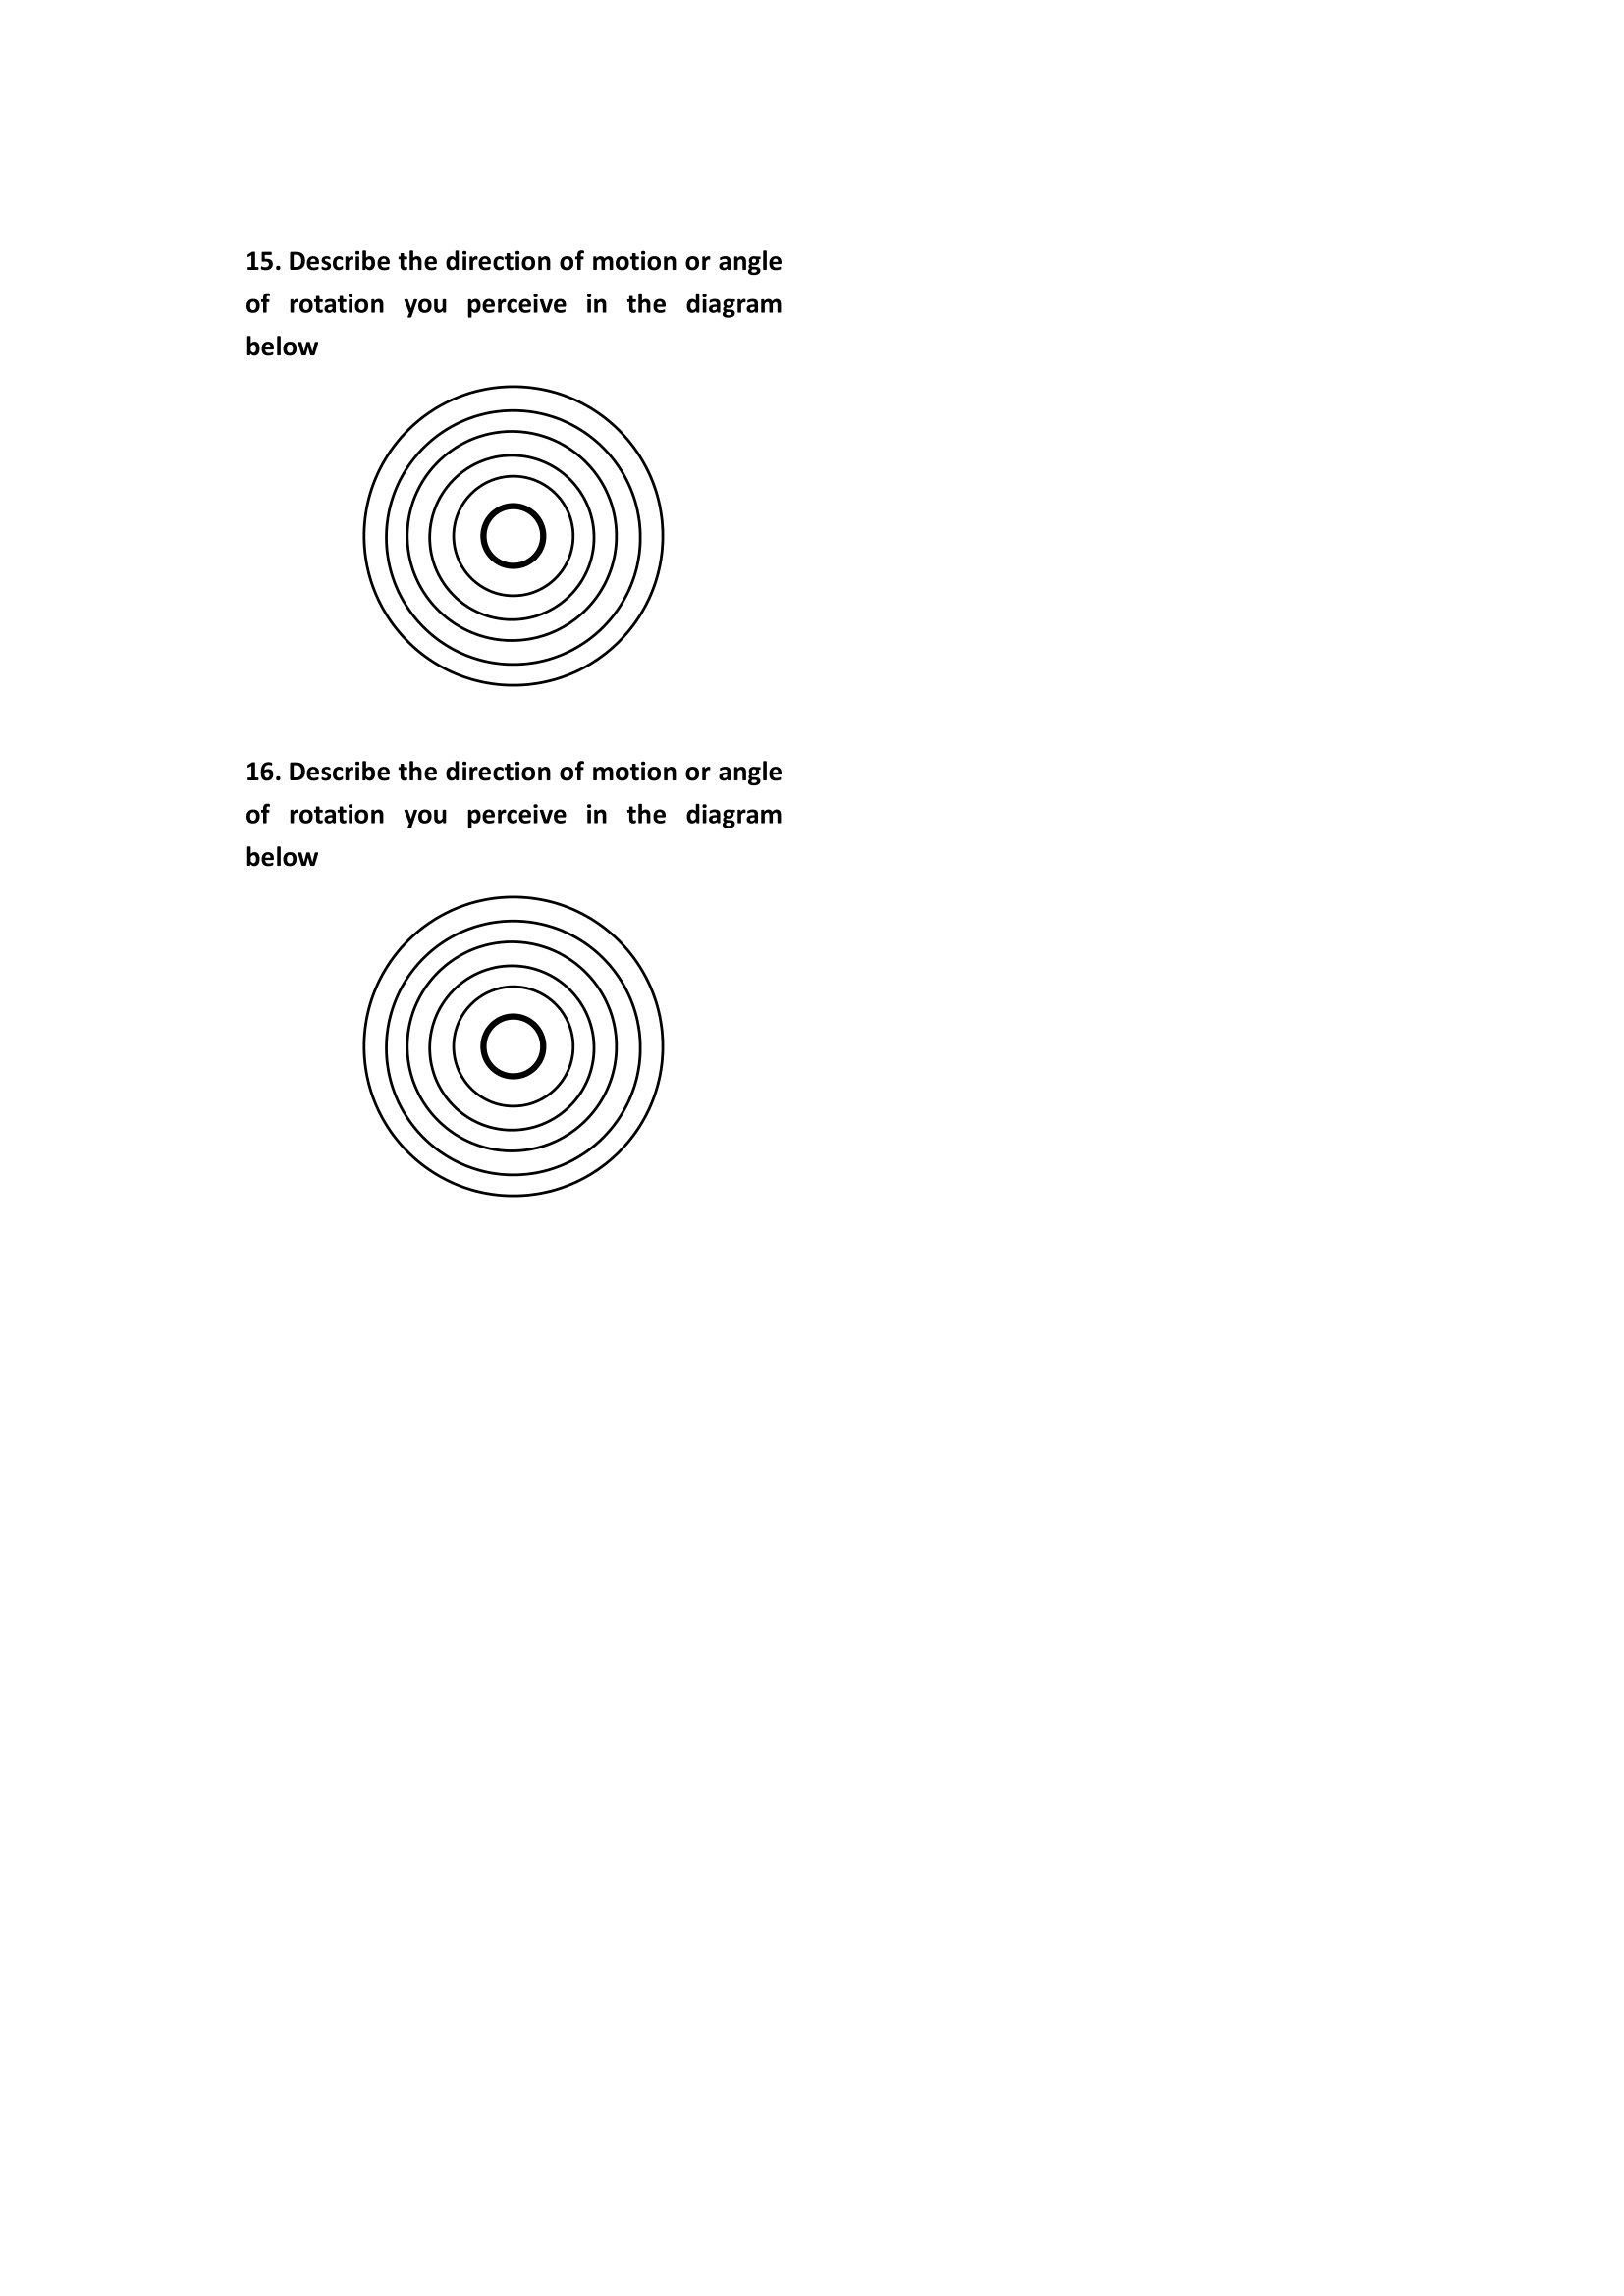
\includegraphics[width=1\textwidth,height=0.7\textheight]{A_thesis/appendix/Experiment1_questionnaire-4.png}
\end{figure}
\newpage

\begin{figure}[h]
\centering
\includegraphics[width=1\textwidth,height=0.7\textheight]{A_thesis/appendix/Experiment1_questionnaire-5.png}
\end{figure}
\newpage

\begin{figure}[h]
\centering
\includegraphics[width=1\textwidth,height=0.7\textheight]{A_thesis/appendix/Experiment1_questionnaire-6.png}
\end{figure}
\newpage

\begin{figure}[h]
\centering
\includegraphics[width=1\textwidth,height=0.7\textheight]{A_thesis/appendix/Experiment1_questionnaire-7.png}
\end{figure}
\newpage

\section{Questionnaire of the Experiment2}
\begin{figure}[h]
\centering
\includegraphics[width=1\textwidth,height=0.7\textheight]{A_thesis/appendix/Experiment 2 3_questionnaire-1.png}
\end{figure}
\newpage

\begin{figure}[h]
\centering
\includegraphics[width=1\textwidth,height=0.7\textheight]{A_thesis/appendix/Experiment 2 3_questionnaire-2.png}
\end{figure}
\newpage

\begin{figure}[h]
\centering
\includegraphics[width=1\textwidth,height=0.7\textheight]{A_thesis/appendix/Experiment 2 3_questionnaire-3.png}
\end{figure}
\newpage

\section{Motion Information Diagram Result}
\begin{figure}[h]
\centering
\includegraphics[width=0.9\textwidth,height=0.36\textheight]{A_thesis/appendix/Exp1_1-01.png}
\break
\break
\includegraphics[width=0.9\textwidth,height=0.36\textheight]{A_thesis/appendix/Exp1_1-02.png}
\end{figure}
\newpage

\begin{figure}[h]
\centering
\includegraphics[width=0.9\textwidth,height=0.36\textheight]{A_thesis/appendix/Exp1_1-03.png}
\break
\break
\includegraphics[width=0.9\textwidth,height=0.36\textheight]{A_thesis/appendix/Exp1_1-04.png}
\end{figure}
\newpage

\begin{figure}[h]
\centering
\includegraphics[width=0.9\textwidth,height=0.36\textheight]{A_thesis/appendix/Exp1_1-05.png}
\break
\break
\includegraphics[width=0.9\textwidth,height=0.36\textheight]{A_thesis/appendix/Exp1_1-06.png}
\end{figure}
\newpage

\begin{figure}[h]
\centering
\includegraphics[width=0.9\textwidth,height=0.36\textheight]{A_thesis/appendix/Exp1_1-07.png}
\break
\break
\includegraphics[width=0.9\textwidth,height=0.36\textheight]{A_thesis/appendix/Exp1_1-08.png}
\end{figure}
\newpage

\begin{figure}[h]
\centering
\includegraphics[width=0.9\textwidth,height=0.36\textheight]{A_thesis/appendix/Exp1_1-09.png}
\break
\break
\includegraphics[width=0.9\textwidth,height=0.36\textheight]{A_thesis/appendix/Exp1_1-10.png}
\end{figure}
\newpage

\begin{figure}[h]
\centering
\includegraphics[width=0.9\textwidth,height=0.36\textheight]{A_thesis/appendix/Exp1_1-11.png}
\break
\break
\includegraphics[width=0.9\textwidth,height=0.36\textheight]{A_thesis/appendix/Exp1_1-12.png}
\end{figure}
\newpage

\section{Questionnaire Result}
\begin{figure}[h]
\centering
\includegraphics[width=1\textwidth,height=0.75\textheight]{A_thesis/appendix/Analysis2 3.xlsx - Exp23-1.png}
\end{figure}



%

\end{document}

% End of File